\documentclass[11pt,oneside]{book}

    \usepackage[italian]{babel}
    \usepackage{subcaption}

    \usepackage[breakable,listings]{tcolorbox}
    \usepackage{parskip} % Stop auto-indenting (to mimic markdown behaviour)
    
    \makeatletter
    % add tcblistings to \jobname.lol (list of listings)
    \tcbset{
      addtolol/.style={list entry={\kvtcb@title},add to list={lol}{chapter}},
      }
    \makeatother
    \renewcommand*{\lstlistlistingname}{Lista dei codici}
    
    \newcommand{\mail}[1]{\href{mailto:#1}{\texttt{#1}}}
    
    \usepackage{iftex}
    \ifPDFTeX
    	\usepackage[T1]{fontenc}
    	\usepackage{mathpazo}
    \else
    	\usepackage{fontspec}
    \fi

    % Basic figure setup, for now with no caption control since it's done
    % automatically by Pandoc (which extracts ![](path) syntax from Markdown).
    \usepackage{graphicx}
    \graphicspath{{./immagini/}}
    % Maintain compatibility with old templates. Remove in nbconvert 6.0
    \let\Oldincludegraphics\includegraphics
    
    \usepackage{float}
    \floatplacement{figure}{H} % forces figures to be placed at the correct location
    \usepackage{xcolor} % Allow colors to be defined
    \usepackage{enumerate} % Needed for markdown enumerations to work
    \usepackage{geometry} % Used to adjust the document margins
    \usepackage{amsmath} % Equations
    \usepackage{amssymb} % Equations
    \usepackage{textcomp} % defines textquotesingle
    % Hack from http://tex.stackexchange.com/a/47451/13684:
    \AtBeginDocument{%
        \def\PYZsq{\textquotesingle}% Upright quotes in Pygmentized code
    }
    \usepackage{upquote} % Upright quotes for verbatim code
    \usepackage{eurosym} % defines \euro
    \usepackage[mathletters]{ucs} % Extended unicode (utf-8) support
    \usepackage{fancyvrb} % verbatim replacement that allows latex
    \usepackage{grffile} % extends the file name processing of package graphics 
                         % to support a larger range
    \makeatletter % fix for old versions of grffile with XeLaTeX
    \@ifpackagelater{grffile}{2019/11/01}
    {
      % Do nothing on new versions
    }
    {
      \def\Gread@@xetex#1{%
        \IfFileExists{"\Gin@base".bb}%
        {\Gread@eps{\Gin@base.bb}}%
        {\Gread@@xetex@aux#1}%
      }
    }
    \makeatother
    \usepackage[Export]{adjustbox} % Used to constrain images to a maximum size
    \adjustboxset{max size={0.9\linewidth}{0.9\paperheight}}

    % The hyperref package gives us a pdf with properly built
    % internal navigation ('pdf bookmarks' for the table of contents,
    % internal cross-reference links, web links for URLs, etc.)
    \usepackage{hyperref}
    % The default LaTeX title has an obnoxious amount of whitespace. By default,
    % titling removes some of it. It also provides customization options.
    \usepackage{titling}
    \usepackage{longtable} % longtable support required by pandoc >1.10
    \usepackage{booktabs}  % table support for pandoc > 1.12.2
    \usepackage[inline]{enumitem} % IRkernel/repr support (it uses the enumerate* environment)
    \usepackage[normalem]{ulem} % ulem is needed to support strikethroughs (\sout)
                                % normalem makes italics be italics, not underlines
    \usepackage{mathrsfs}
    

    
    % Colors for the hyperref package
    \definecolor{urlcolor}{rgb}{0,.145,.698}
    \definecolor{linkcolor}{rgb}{.71,0.21,0.01}
    \definecolor{citecolor}{rgb}{.12,.54,.11}

    % ANSI colors
    \definecolor{ansi-black}{HTML}{3E424D}
    \definecolor{ansi-black-intense}{HTML}{282C36}
    \definecolor{ansi-red}{HTML}{E75C58}
    \definecolor{ansi-red-intense}{HTML}{B22B31}
    \definecolor{ansi-green}{HTML}{00A250}
    \definecolor{ansi-green-intense}{HTML}{007427}
    \definecolor{ansi-yellow}{HTML}{DDB62B}
    \definecolor{ansi-yellow-intense}{HTML}{B27D12}
    \definecolor{ansi-blue}{HTML}{208FFB}
    \definecolor{ansi-blue-intense}{HTML}{0065CA}
    \definecolor{ansi-magenta}{HTML}{D160C4}
    \definecolor{ansi-magenta-intense}{HTML}{A03196}
    \definecolor{ansi-cyan}{HTML}{60C6C8}
    \definecolor{ansi-cyan-intense}{HTML}{258F8F}
    \definecolor{ansi-white}{HTML}{C5C1B4}
    \definecolor{ansi-white-intense}{HTML}{A1A6B2}
    \definecolor{ansi-default-inverse-fg}{HTML}{FFFFFF}
    \definecolor{ansi-default-inverse-bg}{HTML}{000000}

    % common color for the border for error outputs.
    \definecolor{outerrorbackground}{HTML}{FFDFDF}

    % commands and environments needed by pandoc snippets
    % extracted from the output of `pandoc -s`
    \providecommand{\tightlist}{%
      \setlength{\itemsep}{0pt}\setlength{\parskip}{0pt}}
    \DefineVerbatimEnvironment{Highlighting}{Verbatim}{commandchars=\\\{\}}
    % Add ',fontsize=\small' for more characters per line
    \newenvironment{Shaded}{}{}
    \newcommand{\KeywordTok}[1]{\textcolor[rgb]{0.00,0.44,0.13}{\textbf{{#1}}}}
    \newcommand{\DataTypeTok}[1]{\textcolor[rgb]{0.56,0.13,0.00}{{#1}}}
    \newcommand{\DecValTok}[1]{\textcolor[rgb]{0.25,0.63,0.44}{{#1}}}
    \newcommand{\BaseNTok}[1]{\textcolor[rgb]{0.25,0.63,0.44}{{#1}}}
    \newcommand{\FloatTok}[1]{\textcolor[rgb]{0.25,0.63,0.44}{{#1}}}
    \newcommand{\CharTok}[1]{\textcolor[rgb]{0.25,0.44,0.63}{{#1}}}
    \newcommand{\StringTok}[1]{\textcolor[rgb]{0.25,0.44,0.63}{{#1}}}
    \newcommand{\CommentTok}[1]{\textcolor[rgb]{0.38,0.63,0.69}{\textit{{#1}}}}
    \newcommand{\OtherTok}[1]{\textcolor[rgb]{0.00,0.44,0.13}{{#1}}}
    \newcommand{\AlertTok}[1]{\textcolor[rgb]{1.00,0.00,0.00}{\textbf{{#1}}}}
    \newcommand{\FunctionTok}[1]{\textcolor[rgb]{0.02,0.16,0.49}{{#1}}}
    \newcommand{\RegionMarkerTok}[1]{{#1}}
    \newcommand{\ErrorTok}[1]{\textcolor[rgb]{1.00,0.00,0.00}{\textbf{{#1}}}}
    \newcommand{\NormalTok}[1]{{#1}}
    
    % Additional commands for more recent versions of Pandoc
    \newcommand{\ConstantTok}[1]{\textcolor[rgb]{0.53,0.00,0.00}{{#1}}}
    \newcommand{\SpecialCharTok}[1]{\textcolor[rgb]{0.25,0.44,0.63}{{#1}}}
    \newcommand{\VerbatimStringTok}[1]{\textcolor[rgb]{0.25,0.44,0.63}{{#1}}}
    \newcommand{\SpecialStringTok}[1]{\textcolor[rgb]{0.73,0.40,0.53}{{#1}}}
    \newcommand{\ImportTok}[1]{{#1}}
    \newcommand{\DocumentationTok}[1]{\textcolor[rgb]{0.73,0.13,0.13}{\textit{{#1}}}}
    \newcommand{\AnnotationTok}[1]{\textcolor[rgb]{0.38,0.63,0.69}{\textbf{\textit{{#1}}}}}
    \newcommand{\CommentVarTok}[1]{\textcolor[rgb]{0.38,0.63,0.69}{\textbf{\textit{{#1}}}}}
    \newcommand{\VariableTok}[1]{\textcolor[rgb]{0.10,0.09,0.49}{{#1}}}
    \newcommand{\ControlFlowTok}[1]{\textcolor[rgb]{0.00,0.44,0.13}{\textbf{{#1}}}}
    \newcommand{\OperatorTok}[1]{\textcolor[rgb]{0.40,0.40,0.40}{{#1}}}
    \newcommand{\BuiltInTok}[1]{{#1}}
    \newcommand{\ExtensionTok}[1]{{#1}}
    \newcommand{\PreprocessorTok}[1]{\textcolor[rgb]{0.74,0.48,0.00}{{#1}}}
    \newcommand{\AttributeTok}[1]{\textcolor[rgb]{0.49,0.56,0.16}{{#1}}}
    \newcommand{\InformationTok}[1]{\textcolor[rgb]{0.38,0.63,0.69}{\textbf{\textit{{#1}}}}}
    \newcommand{\WarningTok}[1]{\textcolor[rgb]{0.38,0.63,0.69}{\textbf{\textit{{#1}}}}}
    
    
    % Define a nice break command that doesn't care if a line doesn't already
    % exist.
    \def\br{\hspace*{\fill} \\* }
    % Math Jax compatibility definitions
    \def\gt{>}
    \def\lt{<}
    \let\Oldtex\TeX
    \let\Oldlatex\LaTeX
    \renewcommand{\TeX}{\textrm{\Oldtex}}
    \renewcommand{\LaTeX}{\textrm{\Oldlatex}}
    % Document parameters
    % Document title
    \title{lesson\_1\_codice}
    
    
    
    
    
% Pygments definitions
\makeatletter
\def\PY@reset{\let\PY@it=\relax \let\PY@bf=\relax%
    \let\PY@ul=\relax \let\PY@tc=\relax%
    \let\PY@bc=\relax \let\PY@ff=\relax}
\def\PY@tok#1{\csname PY@tok@#1\endcsname}
\def\PY@toks#1+{\ifx\relax#1\empty\else%
    \PY@tok{#1}\expandafter\PY@toks\fi}
\def\PY@do#1{\PY@bc{\PY@tc{\PY@ul{%
    \PY@it{\PY@bf{\PY@ff{#1}}}}}}}
\def\PY#1#2{\PY@reset\PY@toks#1+\relax+\PY@do{#2}}

\expandafter\def\csname PY@tok@w\endcsname{\def\PY@tc##1{\textcolor[rgb]{0.73,0.73,0.73}{##1}}}
\expandafter\def\csname PY@tok@c\endcsname{\let\PY@it=\textit\def\PY@tc##1{\textcolor[rgb]{0.25,0.50,0.50}{##1}}}
\expandafter\def\csname PY@tok@cp\endcsname{\def\PY@tc##1{\textcolor[rgb]{0.74,0.48,0.00}{##1}}}
\expandafter\def\csname PY@tok@k\endcsname{\let\PY@bf=\textbf\def\PY@tc##1{\textcolor[rgb]{0.00,0.50,0.00}{##1}}}
\expandafter\def\csname PY@tok@kp\endcsname{\def\PY@tc##1{\textcolor[rgb]{0.00,0.50,0.00}{##1}}}
\expandafter\def\csname PY@tok@kt\endcsname{\def\PY@tc##1{\textcolor[rgb]{0.69,0.00,0.25}{##1}}}
\expandafter\def\csname PY@tok@o\endcsname{\def\PY@tc##1{\textcolor[rgb]{0.40,0.40,0.40}{##1}}}
\expandafter\def\csname PY@tok@ow\endcsname{\let\PY@bf=\textbf\def\PY@tc##1{\textcolor[rgb]{0.67,0.13,1.00}{##1}}}
\expandafter\def\csname PY@tok@nb\endcsname{\def\PY@tc##1{\textcolor[rgb]{0.00,0.50,0.00}{##1}}}
\expandafter\def\csname PY@tok@nf\endcsname{\def\PY@tc##1{\textcolor[rgb]{0.00,0.00,1.00}{##1}}}
\expandafter\def\csname PY@tok@nc\endcsname{\let\PY@bf=\textbf\def\PY@tc##1{\textcolor[rgb]{0.00,0.00,1.00}{##1}}}
\expandafter\def\csname PY@tok@nn\endcsname{\let\PY@bf=\textbf\def\PY@tc##1{\textcolor[rgb]{0.00,0.00,1.00}{##1}}}
\expandafter\def\csname PY@tok@ne\endcsname{\let\PY@bf=\textbf\def\PY@tc##1{\textcolor[rgb]{0.82,0.25,0.23}{##1}}}
\expandafter\def\csname PY@tok@nv\endcsname{\def\PY@tc##1{\textcolor[rgb]{0.10,0.09,0.49}{##1}}}
\expandafter\def\csname PY@tok@no\endcsname{\def\PY@tc##1{\textcolor[rgb]{0.53,0.00,0.00}{##1}}}
\expandafter\def\csname PY@tok@nl\endcsname{\def\PY@tc##1{\textcolor[rgb]{0.63,0.63,0.00}{##1}}}
\expandafter\def\csname PY@tok@ni\endcsname{\let\PY@bf=\textbf\def\PY@tc##1{\textcolor[rgb]{0.60,0.60,0.60}{##1}}}
\expandafter\def\csname PY@tok@na\endcsname{\def\PY@tc##1{\textcolor[rgb]{0.49,0.56,0.16}{##1}}}
\expandafter\def\csname PY@tok@nt\endcsname{\let\PY@bf=\textbf\def\PY@tc##1{\textcolor[rgb]{0.00,0.50,0.00}{##1}}}
\expandafter\def\csname PY@tok@nd\endcsname{\def\PY@tc##1{\textcolor[rgb]{0.67,0.13,1.00}{##1}}}
\expandafter\def\csname PY@tok@s\endcsname{\def\PY@tc##1{\textcolor[rgb]{0.73,0.13,0.13}{##1}}}
\expandafter\def\csname PY@tok@sd\endcsname{\let\PY@it=\textit\def\PY@tc##1{\textcolor[rgb]{0.73,0.13,0.13}{##1}}}
\expandafter\def\csname PY@tok@si\endcsname{\let\PY@bf=\textbf\def\PY@tc##1{\textcolor[rgb]{0.73,0.40,0.53}{##1}}}
\expandafter\def\csname PY@tok@se\endcsname{\let\PY@bf=\textbf\def\PY@tc##1{\textcolor[rgb]{0.73,0.40,0.13}{##1}}}
\expandafter\def\csname PY@tok@sr\endcsname{\def\PY@tc##1{\textcolor[rgb]{0.73,0.40,0.53}{##1}}}
\expandafter\def\csname PY@tok@ss\endcsname{\def\PY@tc##1{\textcolor[rgb]{0.10,0.09,0.49}{##1}}}
\expandafter\def\csname PY@tok@sx\endcsname{\def\PY@tc##1{\textcolor[rgb]{0.00,0.50,0.00}{##1}}}
\expandafter\def\csname PY@tok@m\endcsname{\def\PY@tc##1{\textcolor[rgb]{0.40,0.40,0.40}{##1}}}
\expandafter\def\csname PY@tok@gh\endcsname{\let\PY@bf=\textbf\def\PY@tc##1{\textcolor[rgb]{0.00,0.00,0.50}{##1}}}
\expandafter\def\csname PY@tok@gu\endcsname{\let\PY@bf=\textbf\def\PY@tc##1{\textcolor[rgb]{0.50,0.00,0.50}{##1}}}
\expandafter\def\csname PY@tok@gd\endcsname{\def\PY@tc##1{\textcolor[rgb]{0.63,0.00,0.00}{##1}}}
\expandafter\def\csname PY@tok@gi\endcsname{\def\PY@tc##1{\textcolor[rgb]{0.00,0.63,0.00}{##1}}}
\expandafter\def\csname PY@tok@gr\endcsname{\def\PY@tc##1{\textcolor[rgb]{1.00,0.00,0.00}{##1}}}
\expandafter\def\csname PY@tok@ge\endcsname{\let\PY@it=\textit}
\expandafter\def\csname PY@tok@gs\endcsname{\let\PY@bf=\textbf}
\expandafter\def\csname PY@tok@gp\endcsname{\let\PY@bf=\textbf\def\PY@tc##1{\textcolor[rgb]{0.00,0.00,0.50}{##1}}}
\expandafter\def\csname PY@tok@go\endcsname{\def\PY@tc##1{\textcolor[rgb]{0.53,0.53,0.53}{##1}}}
\expandafter\def\csname PY@tok@gt\endcsname{\def\PY@tc##1{\textcolor[rgb]{0.00,0.27,0.87}{##1}}}
\expandafter\def\csname PY@tok@err\endcsname{\def\PY@bc##1{\setlength{\fboxsep}{0pt}\fcolorbox[rgb]{1.00,0.00,0.00}{1,1,1}{\strut ##1}}}
\expandafter\def\csname PY@tok@kc\endcsname{\let\PY@bf=\textbf\def\PY@tc##1{\textcolor[rgb]{0.00,0.50,0.00}{##1}}}
\expandafter\def\csname PY@tok@kd\endcsname{\let\PY@bf=\textbf\def\PY@tc##1{\textcolor[rgb]{0.00,0.50,0.00}{##1}}}
\expandafter\def\csname PY@tok@kn\endcsname{\let\PY@bf=\textbf\def\PY@tc##1{\textcolor[rgb]{0.00,0.50,0.00}{##1}}}
\expandafter\def\csname PY@tok@kr\endcsname{\let\PY@bf=\textbf\def\PY@tc##1{\textcolor[rgb]{0.00,0.50,0.00}{##1}}}
\expandafter\def\csname PY@tok@bp\endcsname{\def\PY@tc##1{\textcolor[rgb]{0.00,0.50,0.00}{##1}}}
\expandafter\def\csname PY@tok@fm\endcsname{\def\PY@tc##1{\textcolor[rgb]{0.00,0.00,1.00}{##1}}}
\expandafter\def\csname PY@tok@vc\endcsname{\def\PY@tc##1{\textcolor[rgb]{0.10,0.09,0.49}{##1}}}
\expandafter\def\csname PY@tok@vg\endcsname{\def\PY@tc##1{\textcolor[rgb]{0.10,0.09,0.49}{##1}}}
\expandafter\def\csname PY@tok@vi\endcsname{\def\PY@tc##1{\textcolor[rgb]{0.10,0.09,0.49}{##1}}}
\expandafter\def\csname PY@tok@vm\endcsname{\def\PY@tc##1{\textcolor[rgb]{0.10,0.09,0.49}{##1}}}
\expandafter\def\csname PY@tok@sa\endcsname{\def\PY@tc##1{\textcolor[rgb]{0.73,0.13,0.13}{##1}}}
\expandafter\def\csname PY@tok@sb\endcsname{\def\PY@tc##1{\textcolor[rgb]{0.73,0.13,0.13}{##1}}}
\expandafter\def\csname PY@tok@sc\endcsname{\def\PY@tc##1{\textcolor[rgb]{0.73,0.13,0.13}{##1}}}
\expandafter\def\csname PY@tok@dl\endcsname{\def\PY@tc##1{\textcolor[rgb]{0.73,0.13,0.13}{##1}}}
\expandafter\def\csname PY@tok@s2\endcsname{\def\PY@tc##1{\textcolor[rgb]{0.73,0.13,0.13}{##1}}}
\expandafter\def\csname PY@tok@sh\endcsname{\def\PY@tc##1{\textcolor[rgb]{0.73,0.13,0.13}{##1}}}
\expandafter\def\csname PY@tok@s1\endcsname{\def\PY@tc##1{\textcolor[rgb]{0.73,0.13,0.13}{##1}}}
\expandafter\def\csname PY@tok@mb\endcsname{\def\PY@tc##1{\textcolor[rgb]{0.40,0.40,0.40}{##1}}}
\expandafter\def\csname PY@tok@mf\endcsname{\def\PY@tc##1{\textcolor[rgb]{0.40,0.40,0.40}{##1}}}
\expandafter\def\csname PY@tok@mh\endcsname{\def\PY@tc##1{\textcolor[rgb]{0.40,0.40,0.40}{##1}}}
\expandafter\def\csname PY@tok@mi\endcsname{\def\PY@tc##1{\textcolor[rgb]{0.40,0.40,0.40}{##1}}}
\expandafter\def\csname PY@tok@il\endcsname{\def\PY@tc##1{\textcolor[rgb]{0.40,0.40,0.40}{##1}}}
\expandafter\def\csname PY@tok@mo\endcsname{\def\PY@tc##1{\textcolor[rgb]{0.40,0.40,0.40}{##1}}}
\expandafter\def\csname PY@tok@ch\endcsname{\let\PY@it=\textit\def\PY@tc##1{\textcolor[rgb]{0.25,0.50,0.50}{##1}}}
\expandafter\def\csname PY@tok@cm\endcsname{\let\PY@it=\textit\def\PY@tc##1{\textcolor[rgb]{0.25,0.50,0.50}{##1}}}
\expandafter\def\csname PY@tok@cpf\endcsname{\let\PY@it=\textit\def\PY@tc##1{\textcolor[rgb]{0.25,0.50,0.50}{##1}}}
\expandafter\def\csname PY@tok@c1\endcsname{\let\PY@it=\textit\def\PY@tc##1{\textcolor[rgb]{0.25,0.50,0.50}{##1}}}
\expandafter\def\csname PY@tok@cs\endcsname{\let\PY@it=\textit\def\PY@tc##1{\textcolor[rgb]{0.25,0.50,0.50}{##1}}}

\def\PYZbs{\char`\\}
\def\PYZus{\char`\_}
\def\PYZob{\char`\{}
\def\PYZcb{\char`\}}
\def\PYZca{\char`\^}
\def\PYZam{\char`\&}
\def\PYZlt{\char`\<}
\def\PYZgt{\char`\>}
\def\PYZsh{\char`\#}
\def\PYZpc{\char`\%}
\def\PYZdl{\char`\$}
\def\PYZhy{\char`\-}
\def\PYZsq{\char`\'}
\def\PYZdq{\char`\"}
\def\PYZti{\char`\~}
% for compatibility with earlier versions
\def\PYZat{@}
\def\PYZlb{[}
\def\PYZrb{]}
\makeatother


    % For linebreaks inside Verbatim environment from package fancyvrb. 
    \makeatletter
        \newbox\Wrappedcontinuationbox 
        \newbox\Wrappedvisiblespacebox 
        \newcommand*\Wrappedvisiblespace {\textcolor{red}{\textvisiblespace}} 
        \newcommand*\Wrappedcontinuationsymbol {\textcolor{red}{\llap{\tiny$\m@th\hookrightarrow$}}} 
        \newcommand*\Wrappedcontinuationindent {3ex } 
        \newcommand*\Wrappedafterbreak {\kern\Wrappedcontinuationindent\copy\Wrappedcontinuationbox} 
        % Take advantage of the already applied Pygments mark-up to insert 
        % potential linebreaks for TeX processing. 
        %        {, <, #, %, $, ' and ": go to next line. 
        %        _, }, ^, &, >, - and ~: stay at end of broken line. 
        % Use of \textquotesingle for straight quote. 
        \newcommand*\Wrappedbreaksatspecials {% 
            \def\PYGZus{\discretionary{\char`\_}{\Wrappedafterbreak}{\char`\_}}% 
            \def\PYGZob{\discretionary{}{\Wrappedafterbreak\char`\{}{\char`\{}}% 
            \def\PYGZcb{\discretionary{\char`\}}{\Wrappedafterbreak}{\char`\}}}% 
            \def\PYGZca{\discretionary{\char`\^}{\Wrappedafterbreak}{\char`\^}}% 
            \def\PYGZam{\discretionary{\char`\&}{\Wrappedafterbreak}{\char`\&}}% 
            \def\PYGZlt{\discretionary{}{\Wrappedafterbreak\char`\<}{\char`\<}}% 
            \def\PYGZgt{\discretionary{\char`\>}{\Wrappedafterbreak}{\char`\>}}% 
            \def\PYGZsh{\discretionary{}{\Wrappedafterbreak\char`\#}{\char`\#}}% 
            \def\PYGZpc{\discretionary{}{\Wrappedafterbreak\char`\%}{\char`\%}}% 
            \def\PYGZdl{\discretionary{}{\Wrappedafterbreak\char`\$}{\char`\$}}% 
            \def\PYGZhy{\discretionary{\char`\-}{\Wrappedafterbreak}{\char`\-}}% 
            \def\PYGZsq{\discretionary{}{\Wrappedafterbreak\textquotesingle}{\textquotesingle}}% 
            \def\PYGZdq{\discretionary{}{\Wrappedafterbreak\char`\"}{\char`\"}}% 
            \def\PYGZti{\discretionary{\char`\~}{\Wrappedafterbreak}{\char`\~}}% 
        } 
        % Some characters . , ; ? ! / are not pygmentized. 
        % This macro makes them "active" and they will insert potential linebreaks 
        \newcommand*\Wrappedbreaksatpunct {% 
            \lccode`\~`\.\lowercase{\def~}{\discretionary{\hbox{\char`\.}}{\Wrappedafterbreak}{\hbox{\char`\.}}}% 
            \lccode`\~`\,\lowercase{\def~}{\discretionary{\hbox{\char`\,}}{\Wrappedafterbreak}{\hbox{\char`\,}}}% 
            \lccode`\~`\;\lowercase{\def~}{\discretionary{\hbox{\char`\;}}{\Wrappedafterbreak}{\hbox{\char`\;}}}% 
            \lccode`\~`\:\lowercase{\def~}{\discretionary{\hbox{\char`\:}}{\Wrappedafterbreak}{\hbox{\char`\:}}}% 
            \lccode`\~`\?\lowercase{\def~}{\discretionary{\hbox{\char`\?}}{\Wrappedafterbreak}{\hbox{\char`\?}}}% 
            \lccode`\~`\!\lowercase{\def~}{\discretionary{\hbox{\char`\!}}{\Wrappedafterbreak}{\hbox{\char`\!}}}% 
            \lccode`\~`\/\lowercase{\def~}{\discretionary{\hbox{\char`\/}}{\Wrappedafterbreak}{\hbox{\char`\/}}}% 
            \catcode`\.\active
            \catcode`\,\active 
            \catcode`\;\active
            \catcode`\:\active
            \catcode`\?\active
            \catcode`\!\active
            \catcode`\/\active 
            \lccode`\~`\~ 	
        }
    \makeatother

    \let\OriginalVerbatim=\Verbatim
    \makeatletter
    \renewcommand{\Verbatim}[1][1]{%
        %\parskip\z@skip
        \sbox\Wrappedcontinuationbox {\Wrappedcontinuationsymbol}%
        \sbox\Wrappedvisiblespacebox {\FV@SetupFont\Wrappedvisiblespace}%
        \def\FancyVerbFormatLine ##1{\hsize\linewidth
            \vtop{\raggedright\hyphenpenalty\z@\exhyphenpenalty\z@
                \doublehyphendemerits\z@\finalhyphendemerits\z@
                \strut ##1\strut}%
        }%
        % If the linebreak is at a space, the latter will be displayed as visible
        % space at end of first line, and a continuation symbol starts next line.
        % Stretch/shrink are however usually zero for typewriter font.
        \def\FV@Space {%
            \nobreak\hskip\z@ plus\fontdimen3\font minus\fontdimen4\font
            \discretionary{\copy\Wrappedvisiblespacebox}{\Wrappedafterbreak}
            {\kern\fontdimen2\font}%
        }%
        
        % Allow breaks at special characters using \PYG... macros.
        \Wrappedbreaksatspecials
        % Breaks at punctuation characters . , ; ? ! and / need catcode=\active 	
        \OriginalVerbatim[#1,codes*=\Wrappedbreaksatpunct]%
    }
    \makeatother

    % Exact colors from NB
    \definecolor{incolor}{HTML}{303F9F}
    \definecolor{outcolor}{HTML}{D84315}
    \definecolor{cellborder}{HTML}{CFCFCF}
    \definecolor{cellbackground}{HTML}{F7F7F7}
    
    % prompt
    \makeatletter
    \newcommand{\boxspacing}{\kern\kvtcb@left@rule\kern\kvtcb@boxsep}
    \makeatother
    \newcommand{\prompt}[4]{
        {\ttfamily\llap{{\color{#2}[#3]:\hspace{3pt}#4}}\vspace{-\baselineskip}}
    }
    

    
    % Prevent overflowing lines due to hard-to-break entities
    \sloppy 
    % Setup hyperref package
    \hypersetup{
      breaklinks=true,  % so long urls are correctly broken across lines
      colorlinks=true,
      urlcolor=urlcolor,
      linkcolor=linkcolor,
      citecolor=citecolor,
      }
    % Slightly bigger margins than the latex defaults
    
    \geometry{verbose,tmargin=1in,bmargin=1in,lmargin=1in,rmargin=1in}
    
    
% FINE PREAMBOLO GENERATO DA JUPYTER =========================================================
\begin{document}

\begin{titlepage}
    \begin{center}
        
        \Large
        \textbf{Università degli Studi di Verona} \\
        Dipartimento di Informatica \\
        CdLM in Ingegneria e scienze informatiche
        
        \vspace{5cm}
        
        \Huge
        \textcolor{linkcolor}{\textbf{Fondamenti di intelligenza artificiale}}
        
        \vspace{0.5cm}
        \LARGE
        Riassunto del corso
        
        \vspace{5cm}
        
        Creato da: \textbf{Davide Zampieri}
        
        \vfill
        
        \Large
        \textbf{Anno Accademico 2020-2021}
        
    \end{center}
\end{titlepage}

\frontmatter
\tableofcontents
\lstlistoflistings

\mainmatter
\chapter{Introduzione}

\section{Cos'è l'intelligenza artificiale?}
Quando ci si avvicina per la prima volta all'IA è necessario porsi \textit{due domande}:
\begin{enumerate}
    \item Interessa di più il pensiero o il comportamento?
    \item Si vuole usare come modello gli esseri umani o fare riferimento ad uno standard ideale?
\end{enumerate}
Con le \textit{risposte} a queste domande possiamo costruire la seguente tabella:
\begin{center}
	\begin{tabular}{cc}
		\toprule
		Systems that think like humans & Systems that think rationally \\
		\midrule
		Systems that act like humans & Systems that act rationally \\
		\bottomrule
	\end{tabular}
\end{center}

\subsection{Agire razionalmente}
Da questo momento in poi adottiamo l'idea che l'intelligenza riguardi principalmente l'\textit{azione razionale}. Idealmente, un \textit{agente intelligente} intraprende in ogni situazione la migliore azione possibile. Bisognerà quindi trovare il modo di costruire agenti intelligenti secondo questa particolare accezione.


\section{I fondamenti dell'intelligenza artificiale}
I \textit{filosofi}, a partire dal 400 a.C., hanno reso concepibile lo sviluppo dell'IA proponendo che la mente fosse per certi aspetti simile ad una macchina.

I \textit{matematici} hanno poi fornito gli strumenti per manipolare gli enunciati logici (sia in condizioni di certezza che di incertezza), e hanno anche sviluppato la teoria della computazione e dell'analisi di algoritmi.

Inoltre, gli \textit{economisti} hanno formalizzato il problema di prendere decisioni che massimizzino i risultati attesi, mentre gli \textit{studiosi di neuroscienze} hanno scoperto alcuni fatti sul funzionamento del cervello e sui relativi punti di somiglianza e di differenza rispetto ai computer.

Infine, gli \textit{psicologi} e i \textit{linguisti} hanno adottato l'idea che gli esseri umani possano essere considerati macchine che elaborano informazioni, mentre gli \textit{ingegneri informatici} hanno creato macchine sempre più potenti per rendere possibili le applicazioni dell'IA.


\section{La storia dell'intelligenza artificiale}
Attualmente la \textit{teoria del controllo} si sta avvicinando all'IA, in quanto si occupa della progettazione di dispositivi che agiscono in maniera ottimale basandosi sull'ambiente.

Ma la \textit{storia} dell'IA è stata anche segnata da cicli in cui al successo ha fatto seguito un eccessivo ottimismo che ha portato a cadute d'entusiasmo e a tagli di fondi.

Ora, grazie all'introduzione di nuovi approcci creativi e all'uso diffuso del metodo scientifico, i \textit{diversi settori} dell'IA sono arrivati ad un'integrazione e, con l'aumento delle capacità di calcolo dei sistemi, l'IA stessa sta trovando un terreno comune con altre discipline.


\chapter{Agenti intelligenti}

\section{Agenti e ambienti}
Un \textit{agente} è qualcosa che percepisce e agisce all'interno di un \textit{ambiente}. La sua \textit{funzione agente} specifica l'azione intrapresa in risposta a qualsiasi sequenza di percezioni. Formalmente, la funzione agente è definita nel seguente modo:
\[
    f : \mathcal{P}^* \rightarrow \mathcal{A}
\]
dove $\mathcal{P}^*$ è lo storico delle percezioni e $A$ è un insieme di azioni.

Inoltre, si fa notare che se un agente ha $|\mathcal{P}|$ percezioni possibili in ingresso, dopo $T$ unità di tempo la sua funzione agente avrà un numero di entry pari a $\sum_{t=1}^{T} |\mathcal{P}|^t$.

\subsection{Razionalità}
La \textit{misura di prestazione} valuta il comportamento dell'agente nell'ambiente in cui opera. Un agente \textit{razionale} dovrà quindi agire in modo da massimizzare il valore atteso della misura di prestazione (data la sequenza percettiva fino a quel momento).

\section{La natura degli ambienti}
\subsection{Specificare un ambiente}
La specifica di un task environment, o \textit{ambiente operativo}, include:
\begin{itemize}
    \item La misura di \textbf{p}restazione.
    \item L'ambiente \textbf{e}sterno.
    \item Gli \textbf{a}ttuatori.
    \item I \textbf{s}ensori.
\end{itemize}
Nella \textit{progettazione} di un agente razionale il primo passo deve sempre consistere nella specifica più dettagliata possibile dell'ambiente operativo.

\subsection{Proprietà degli ambienti}
Gli ambienti operativi possono essere classificati in base a molte \textit{proprietà} significative. Basandoci su alcune di esse potremo stabilire se gli agenti sono:
\begin{itemize}
	\item Completamente o parzialmente osservabili.
	\item Deterministici o stocastici.
	\item Episodici o sequenziali.
	\item Statici o dinamici.
	\item Discreti o continui.
	\item A singolo agente o multi-agente.
\end{itemize}

\section{La struttura degli agenti}
\subsection{Programmi agente}
Il \textit{programma agente} implementa la funzione agente, ovvero prende in input la percezione attuale e ritorna in output la prossima azione da svolgere.

Esisteranno quindi diversi \textit{schemi} base per tali programmi, che rifletteranno il tipo di informazione esplicitata e utilizzata nel processo decisionale. Siccome gli schemi possono variare in efficienza, compattezza e flessibilità, lo schema più appropriato per un dato programma agente dipenderà dalla natura dell'ambiente stesso.

\subsection{Tipi di agenti}
\begin{figure}[htp]
	\begin{subfigure}{0.49\textwidth}
	    \centering
		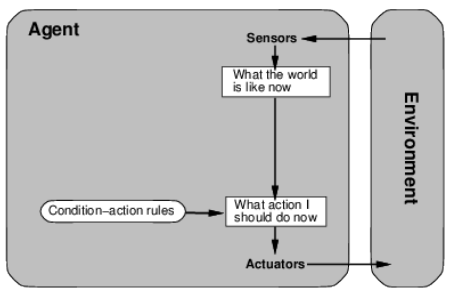
\includegraphics[width=0.75\textwidth]{simple-reflex.png} 
		\caption{Simple reflex agents}
	\end{subfigure}
	\hfill
	\begin{subfigure}{0.49\textwidth}
	    \centering
		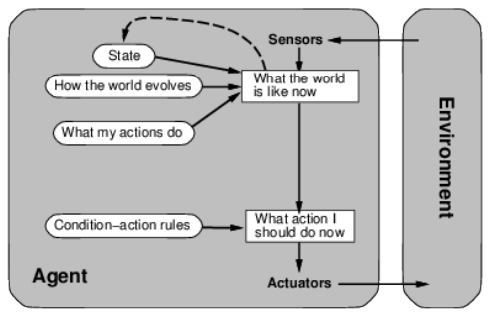
\includegraphics[width=0.75\textwidth]{model-based.png} 
		\caption{Model-based agents}
	\end{subfigure}
	\begin{subfigure}{0.49\textwidth}
	    \centering
		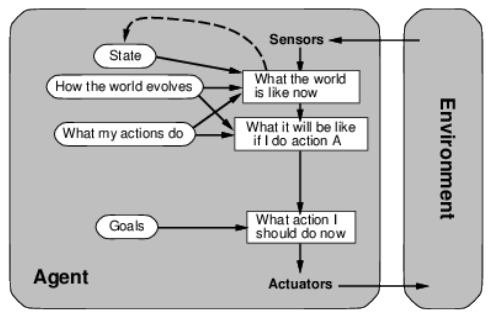
\includegraphics[width=0.75\textwidth]{goal-based.png}
		\caption{Goal-based agents}
	\end{subfigure}
	\hfill
	\begin{subfigure}{0.49\textwidth}
	    \centering
		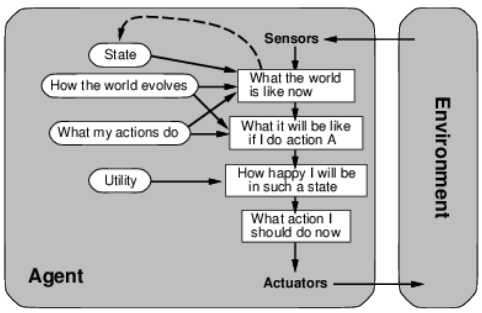
\includegraphics[width=0.75\textwidth]{utility-based.png}
		\caption{Utility-based agents}
	\end{subfigure}
\end{figure}
Esistono principalmente quattro \textit{tipi} di agenti:
\begin{enumerate}[label=(\alph*)]
	\item Gli \textit{agenti reattivi semplici}, che rispondono direttamente alle percezioni.
	\item Gli \textit{agenti reattivi basati su modello}, che mantengono uno stato interno per tener traccia degli aspetti del mondo che non sono visibili nelle percezioni correnti.
	\item Gli \textit{agenti basati su obiettivi}, le cui azioni sono condizionate dall'obiettivo prefissato.
	\item Gli \textit{agenti basati sull'utilità}, che cercano di massimizzare un valore atteso.
\end{enumerate}
Tutte le tipologie di agenti possono migliorare le loro prestazioni mediante l'\textit{apprendimento}.


\chapter{Risolvere i problemi con la ricerca}

\section{Agenti risolutori di problemi}
I \textit{problemi} possono essere:
\begin{enumerate}
	\item Deterministici e completamente osservabili (a stato singolo).
	\item Non osservabili.
	\item Non deterministici e/o parzialmente osservabili.
\end{enumerate}
Nel primo caso, ovvero all'interno di ambienti deterministici, osservabili, statici e completamente noti, l'\textit{agente} può costruire sequenze di azioni che raggiungono il suo obiettivo; questo processo si chiama \textit{ricerca}.

\subsection{La formulazione dei problemi}
Prima di cominciare a cercare le soluzioni, è necessario identificare un \textit{obiettivo} e formulare un \textit{problema} ben definito, il quale è composto da quattro parti:
\begin{enumerate}
	\item Lo \textit{stato iniziale}.
	\item Un \textit{modello di transizione} (successor function) che descrive i risultati di un insieme di \textit{azioni}.
	\item Una funzione \textit{test obiettivo}.
	\item Una funzione \textit{costo di cammino}.
\end{enumerate}
L'ambiente del problema è rappresentato invece dallo \textit{spazio degli stati}. Una \textit{soluzione} è quindi un cammino attraverso lo spazio degli stati che va da uno stato iniziale a uno stato di goal (obiettivo).

\section{Cercare soluzioni}
In generale possiamo avere due tipi di algoritmi di ricerca:
\begin{itemize}
    \item Algoritmi \emph{Tree-Search}, in cui si considerano tutti i possibili cammini.
    \item Algoritmi \emph{Graph-Search}, in cui i cammini ridondanti non vengono presi in considerazione.
\end{itemize}

\subsection{Strutture dati per algoritmi di ricerca}
Le \textit{strutture dati} utilizzate negli algoritmi di ricerca sono:
\begin{itemize}
	\item Una coda FIFO \emph{frontier} contenente i nodi foglia disponibili.
	\item Un insieme di nodi \emph{explored} contenente i nodi della frontiera che sono stati espansi in passi precedenti.
\end{itemize}
Va ricordato inoltre che il \textit{nodo} è una struttura dati che può contenere vari campi, mentre lo \textit{stato} è una rappresentazione fisica della configurazione di un ambiente e quindi non ha campi.
\begin{figure}[htp]
	\begin{subfigure}{0.49\textwidth}
	    \centering
		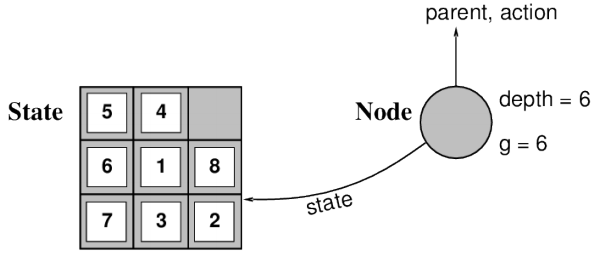
\includegraphics[width=0.8\textwidth]{states-nodes.png} 
		\caption{States vs nodes}
	\end{subfigure}
	\hfill
	\begin{subfigure}{0.49\textwidth}
	    \centering
		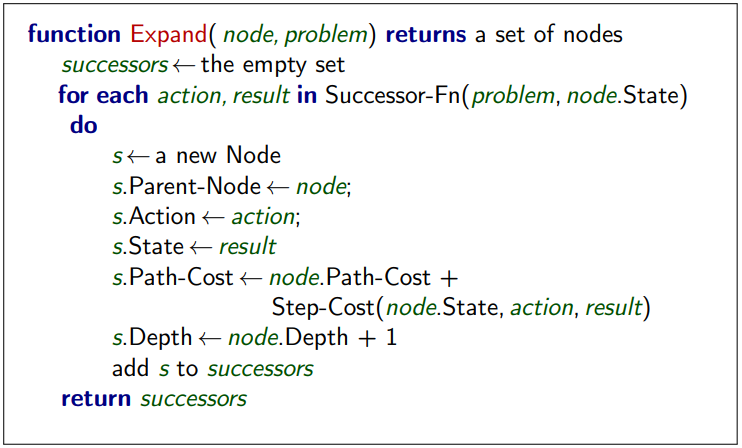
\includegraphics[width=0.8\textwidth]{expand.png} 
		\caption{Expand nodes}
	\end{subfigure}
	\begin{subfigure}{0.49\textwidth}
	    \centering
		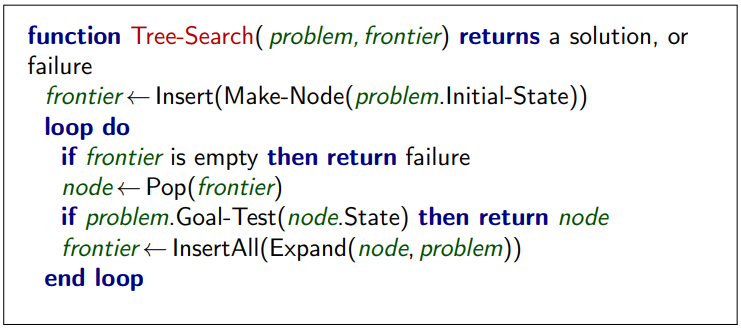
\includegraphics[width=0.8\textwidth]{tree-search.png}
		\caption{Tree search}
	\end{subfigure}
	\hfill
	\begin{subfigure}{0.49\textwidth}
	    \centering
		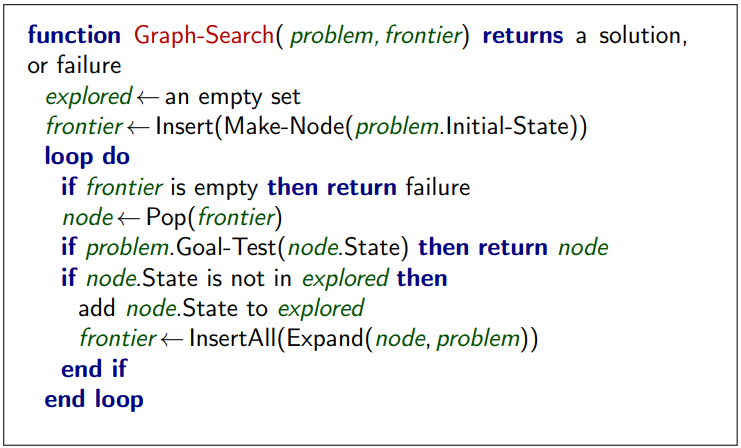
\includegraphics[width=0.8\textwidth]{graph-search.png}
		\caption{Graph search}
	\end{subfigure}
\end{figure}

\subsection{Misurare le prestazioni nella risoluzione di problemi}
Gli algoritmi di ricerca sono valutati sulla base delle seguenti \textit{dimensioni}:
\begin{itemize}
	\item \textit{Completezza}, ovvero se l'algoritmo trova sempre una soluzione quando essa esiste.
	\item \textit{Complessità temporale}, ovvero il numero di nodi generati/espansi.
	\item \textit{Complessità spaziale}, ovvero il massimo numero di nodi da mantenere in memoria.
	\item \textit{Ottimalità}, ovvero se l'algoritmo trova sempre la soluzione a costo minore.
\end{itemize}
La \textit{complessità} dipende da:
\begin{itemize}
	\item \textit{b}, cioè il massimo fattore di ramificazione (\textit{branching factor}) dello spazio degli stati.
	\item \textit{d}, cioè la profondità (\textit{depth}) della soluzione a costo minore (quella più vicina alla radice dell'albero).
	\item \textit{m}, cioè la massima profondità dello spazio degli stati (può essere $\infty$).
\end{itemize}


\section{Strategie di ricerca non informata}
I metodi di \textit{ricerca non informata} hanno accesso soltanto alla definizione del problema. Di seguito vengono presentati i vari algoritmi di base.

\subsection{Ricerca in ampiezza}
L'algoritmo di \textit{ricerca in ampiezza} (Breadth-first search, BFS) espande per primi i nodi più vicini alla radice. La \textit{frontiera} sarà quindi una coda FIFO. Per quanto riguarda le proprietà, la ricerca in ampiezza è \textit{completa} e, quando i passi hanno costo unitario, anche \textit{ottima} (in generale non lo è). Ma il vero problema di questo algoritmo risiede nel fatto che ha una \textit{complessità spaziale} esponenziale dell'ordine di $O(b^d)$; infatti, siccome deve tenere traccia di ogni nodo, più è grande l'albero più spazio verrà occupato in memoria.
\begin{figure}[htp]
	\centering
	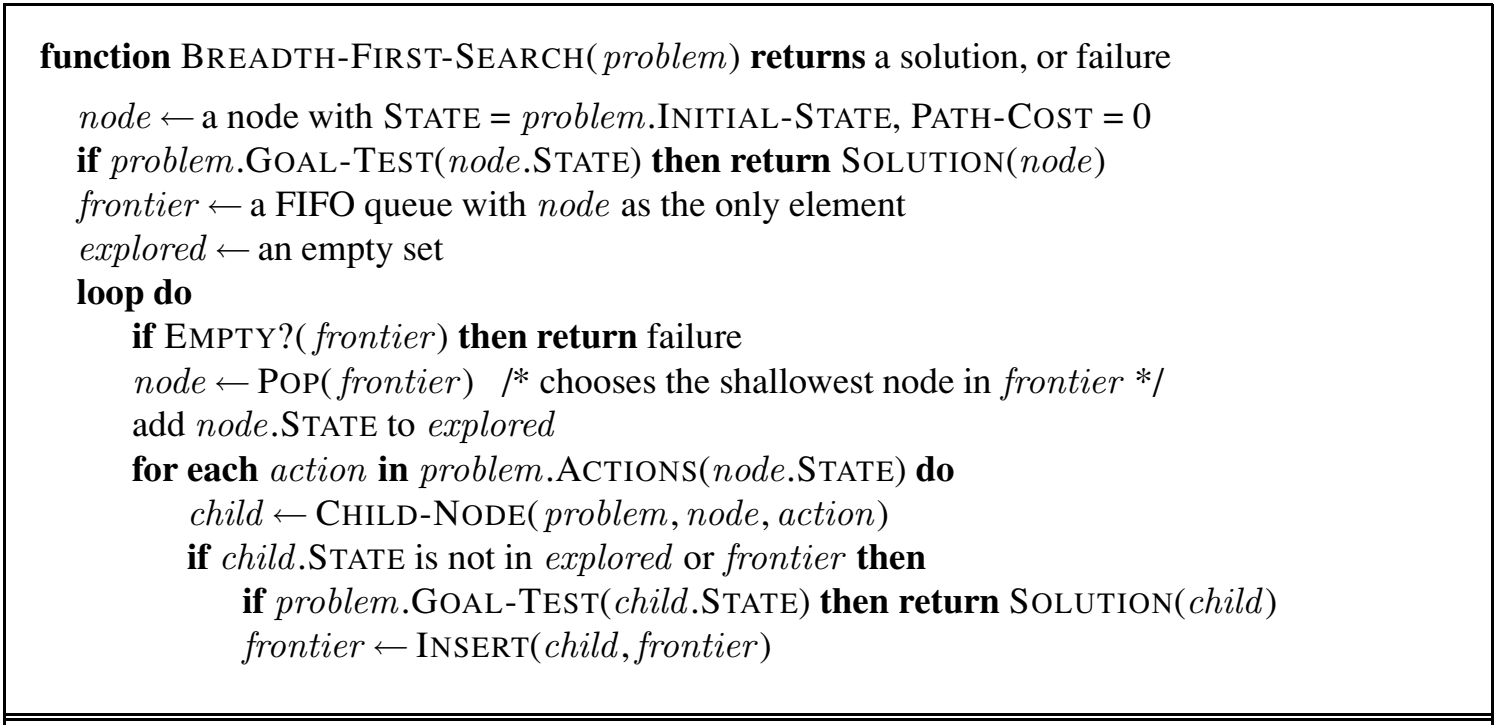
\includegraphics[width=0.7\textwidth]{bfs.png}
\end{figure}

\subsection{Ricerca a costo uniforme}
L'algoritmo di \textit{ricerca a costo uniforme} (Uniform cost search, UCS) espande sempre il nodo che ha il minor costo di cammino. La \textit{frontiera} sarà quindi una coda ordinata per costo in modo crescente. Se tutti i costi sono uguali, questo algoritmo è equivalente alla ricerca in ampiezza. Per quanto riguarda le proprietà, la ricerca a costo uniforme è \textit{completa} e \textit{ottima} per costi di passo qualsiasi.

\subsection{Ricerca in profondità}
L'algoritmo di \textit{ricerca in profondità} (Depth-first search, DFS) espande prima il nodo più profondo non ancora espanso. La \textit{frontiera} sarà quindi una coda LIFO. Per quanto riguarda le proprietà, la ricerca in profondità non è \textit{né completa né ottima}. Tuttavia, la complessità spaziale è lineare in $O(bm)$, che sarebbe ideale se non per il fatto che l'algoritmo fallisce se sono presenti cicli che determinano cammini infiniti (incompletezza).

\subsection{Ricerca ad approfondimento iterativo}
Per gli algoritmi di \textit{ricerca ad approfondimento iterativo} (Iterative deepening search, IDS) ci si serve di un'implementazione ricorsiva di un algoritmo di \textit{ricerca a profondità limitata} (Depth-limited search, DLS), il quale prevede di mettere un limite alla profondità (risolvendo il problema dei cammini infiniti).

La ricerca ad approfondimento iterativo eseguirà quindi una serie di ricerche a profondità limitata, estendendo progressivamente il limite di profondità finché non trova una soluzione. Per quanto riguarda le proprietà, la ricerca ad approfondimento iterativo è \textit{completa} e, quando i passi hanno costo unitario, anche \textit{ottima}. Inoltre, ha una complessità temporale pari a $O(b^d)$ (comparabile alla ricerca in ampiezza) e una complessità spaziale lineare in $O(bd)$.
\begin{figure}[htp]
	\centering
	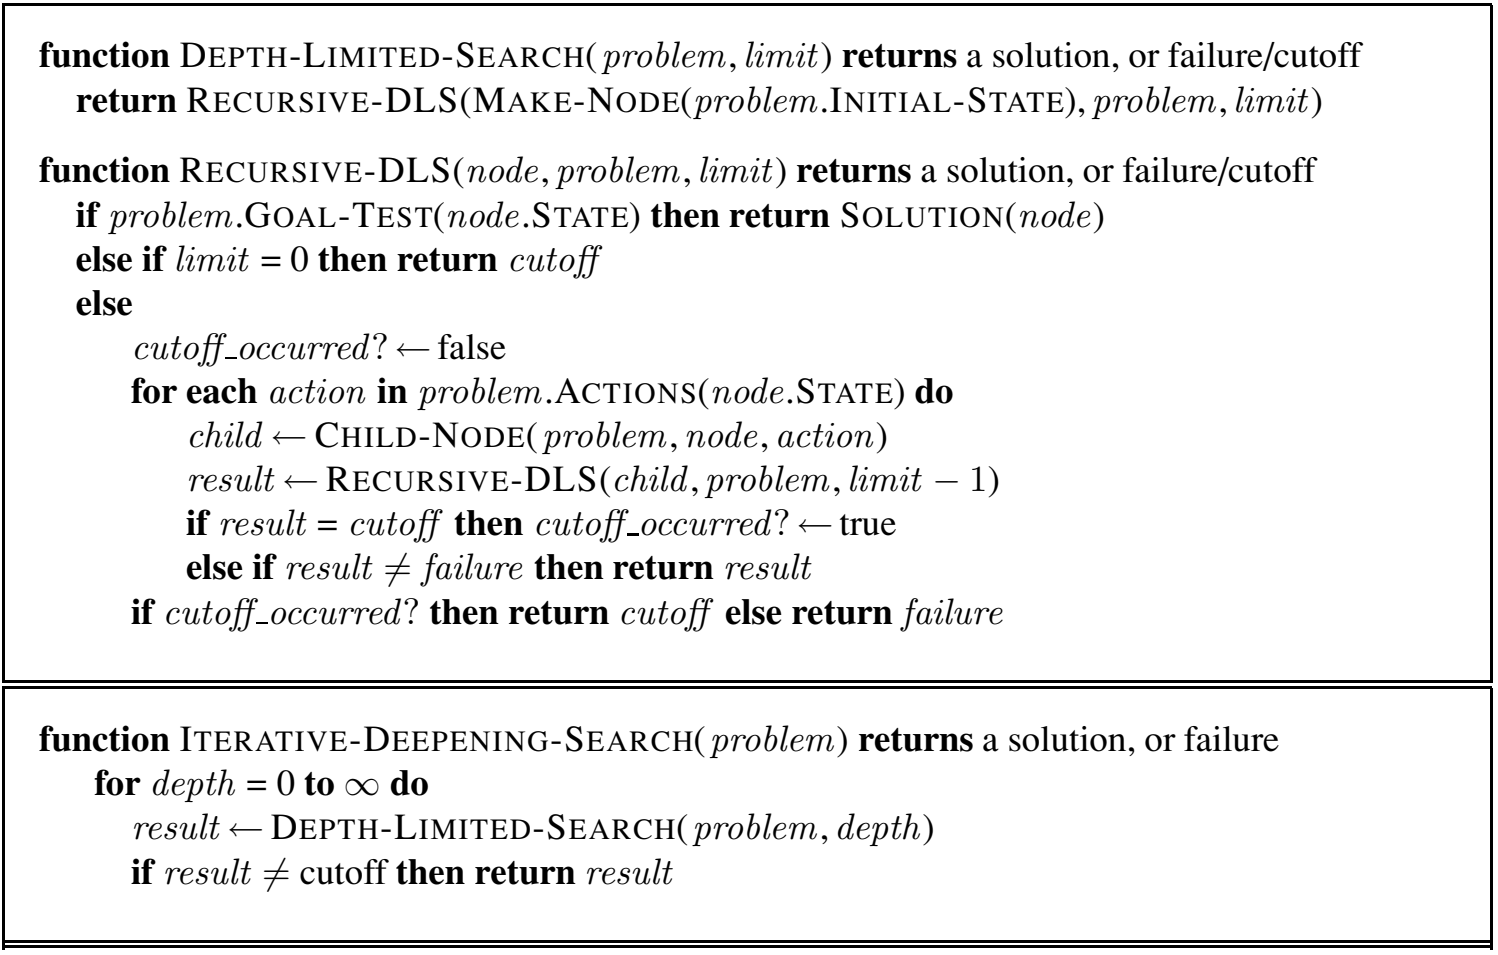
\includegraphics[width=0.7\textwidth]{ids.png}
\end{figure}

\subsection{Confronto tra le strategie di ricerca non informata}
Confrontiamo ora le strategie di ricerca secondo i quattro \textit{criteri di valutazione} (completezza, ottimalità, complessità temporale e spaziale). Tale confronto riguarda le versioni di \textit{ricerca su alberi}. Nelle \textit{ricerche su grafi} la differenza principale è che le complessità spaziali e temporali risultano più efficienti in quanto limitate dalla dimensione dello spazio degli stati.
\begin{center}
	\begin{tabular}{cccccc}
		\toprule
		\textbf{Criterio} & \textbf{BFS} & \textbf{UCS} & \textbf{DFS} & \textbf{DLS} & \textbf{IDS} \\
		
		\midrule
		Completa? & Sì$^a$ & Sì$^{a,b}$ & No & Sì$^{a,d}$ & Sì$^a$ \\
		
		Tempo & $O(b^d)$ & $O(b^{\lceil C^\ast / \epsilon \rceil})$ & $O(b^m)$ & $O(b^l)$ & $O(b^d)$ \\
		
		Spazio & $O(b^d)$ & $O(b^{\lceil C^\ast / \epsilon \rceil})$ & $O(bm)$ & $O(bl)$ & $O(bd)$ \\
		
		Ottima? & Sì$^c$ & Sì & No & Sì$^{c,d}$ & Sì$^c$ \\
		
		\bottomrule
	\end{tabular}
\end{center}
\begin{enumerate}[label=$^{\alph*}$]
	\item completa se il fattore di ramificazione $b$ è finito.
	\item completa se i costi dei passi sono $\geq$ di un $\epsilon$ positivo.
	\item ottima se i costi dei passi sono tutti identici.
	\item se il livello del goal si trova entro il limite.
\end{enumerate}


\newpage
\section{Strategie di ricerca informata o euristica}
Le strategie di \textit{ricerca informata} possono utilizzare conoscenze specifiche riguardanti il problema (oltre alla definizione dello stesso) e pertanto sono più efficienti. In particolare, i metodi di ricerca informata possono avere accesso ad una funzione \textit{euristica} $h(n)$ che stima il costo di una soluzione da $n$. Gli approcci generali sono di due tipi:
\begin{itemize}
	\item Ricerca \textit{greedy best-first}.
	\item Ricerca $A^\ast$.
\end{itemize}

\subsection{Ricerca greedy best-first}
Un algoritmo di \textit{ricerca best-first} generico seleziona un nodo per l'espansione in base ad una \textit{funzione di valutazione} (detta euristica). In particolare, l'approccio di \textit{ricerca greedy best-first} espande i nodi con $h(n)$ minima, ovvero cerca di espandere il nodo che sembra essere il più vicino al goal. Per quanto riguarda le proprietà, la ricerca greedy best-first non è \textit{né completa} (può fallire in caso di cicli) \textit{né ottima}. Inoltre, ha una complessità temporale pari a $O(b^m)$ (migliorabile utilizzando euristiche migliori) e una complessità spaziale a sua volta pari a $O(b^m)$, in quanto è necessario tenere in memoria tutti i nodi.

\subsection{Ricerca \texorpdfstring{$A^\ast$}{A-star}}
La \textit{ricerca} $A^\ast$ espande i nodi con $f(n) = g(n) + h(n)$ minima. L'idea è quella di evitare di espandere percorsi che risultano già essere troppo costosi. Vediamo in dettaglio le componenti della \textit{funzione di valutazione}:
\begin{itemize}
	\item $g(n)$ è il costo per raggiungere $n$.
	\item $h(n)$ è il costo stimato per raggiungere il goal a partire da $n$.
	\item $f(n)$ è il costo stimato totale del percorso che raggiunge il goal attraverso $n$.
\end{itemize}
La ricerca $A^\ast$ usa un'euristica \textit{ammissibile}, ovvero un'euristica in cui $h(n) \leq h^\ast(n)$ dove $h^\ast(n)$ è il vero costo per raggiungere $n$; viene anche richiesto $h(n) \geq 0$, in modo da avere $h(G) = 0$ per ogni goal $G$. Per studiare le proprietà della ricerca $A^\ast$ consideriamo due casi:
\begin{itemize}
    \item $A^\ast$ nella versione \textit{Tree-Search} è \textit{completa} e \textit{ottima}, purché $h(n)$ sia \textit{ammissibile}.
    \item $A^\ast$ nella versione \textit{Graph-Search} è \textit{completa} e \textit{ottima}, purché $h(n)$ sia \textit{consistente}.
\end{itemize}
Si ricorda inoltre che \textit{consistenza} $\rightarrow$ \textit{ammissibilità} ma \textit{ammissibilità} $\not \rightarrow$ \textit{consistenza}. Infine, si fa notare che la complessità spaziale di $A^\ast$ è ancora proibitiva, in quanto deve comunque tenere tutti i nodi in memoria.

\subsection{Funzioni euristiche}
Un'euristica è \textit{consistente} se $h(n) \leq c(n,a,n') + h(n')$ dove $c(n,a,n')$ è il costo per raggiungere $n'$ da $n$. Inoltre, un'euristica $h_2$ \textit{domina} un'altra euristica $h_1$ se $\forall n. \, h_2(n) \geq h_1(n)$. L'euristica dominante sarà quindi sempre migliore dal punto di vista prestazionale. Infine, è bene sapere che talvolta si possono costruire buone euristiche \textit{rilassando} la definizione del problema.


\chapter{Oltre la ricerca classica}

\section{Algoritmi di ricerca locale e problemi di ottimizzazione}
Prenderemo ora in esame algoritmi di ricerca per problemi che vanno oltre il caso \textit{"classico"} di trovare il cammino più breve per arrivare ad un obiettivo in un ambiente osservabile, deterministico e discreto.

\subsection{Ricerca hill climbing}
La ricerca \textit{hill climbing} è un metodo di \textit{ricerca locale} che lavora su formulazioni del problema a stato completo. Si tratta di un semplice ciclo che si muove continuamente verso l'alto, cioè nella direzione dei valori crescenti, e termina quando raggiunge un picco che non ha vicini di valore più alto (\textit{massimo globale}). L'algoritmo mantiene in memoria solo un piccolo numero di nodi.
\begin{figure}[htp]
	\begin{subfigure}{0.49\textwidth}
	    \centering
		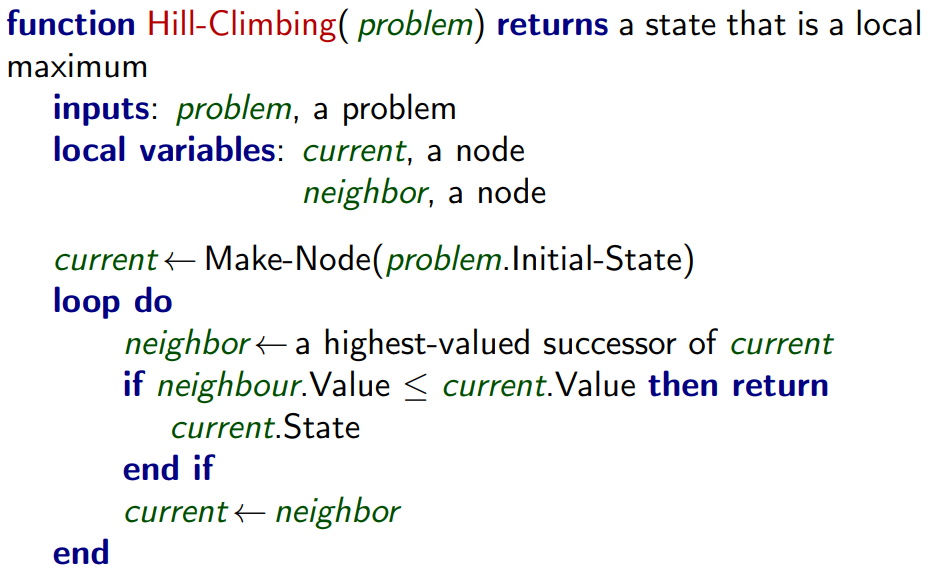
\includegraphics[width=\textwidth, height=\textheight, keepaspectratio]{hill-climbing-1.png} 
		\caption{Algoritmo di ricerca hill climbing}
	\end{subfigure}
	\hfill
	\begin{subfigure}{0.49\textwidth}
	    \centering
		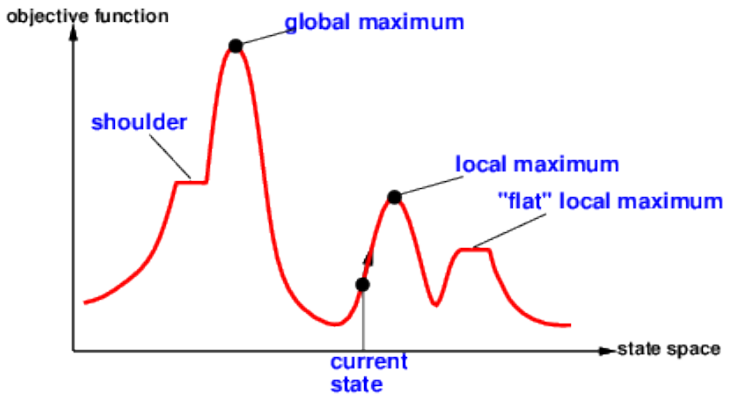
\includegraphics[width=\textwidth, height=\textheight, keepaspectratio]{hill-climbing-2.png} 
		\caption{Spazio degli stati monodimensionale}
	\end{subfigure}
\end{figure}

\subsection{Simulated annealing e algoritmi genetici}
Il \textit{simulated annealing} è un algoritmo stocastico che fornisce soluzioni ottime quando viene impostata una velocità di raffreddamento appropriata (\textit{schedule}). Gli \textit{algoritmi genetici}, invece, sono un particolare tipo di ricerca hill climbing stocastica in cui viene tenuta in memoria una grande popolazione di stati e in cui i nuovi stati vengono generati attraverso la \textit{mutazione} e il \textit{crossover}, il quale genera nuovi individui mediante la combinazione di coppie di stati della popolazione.
\begin{figure}[htp]
	\begin{subfigure}{0.49\textwidth}
	    \centering
		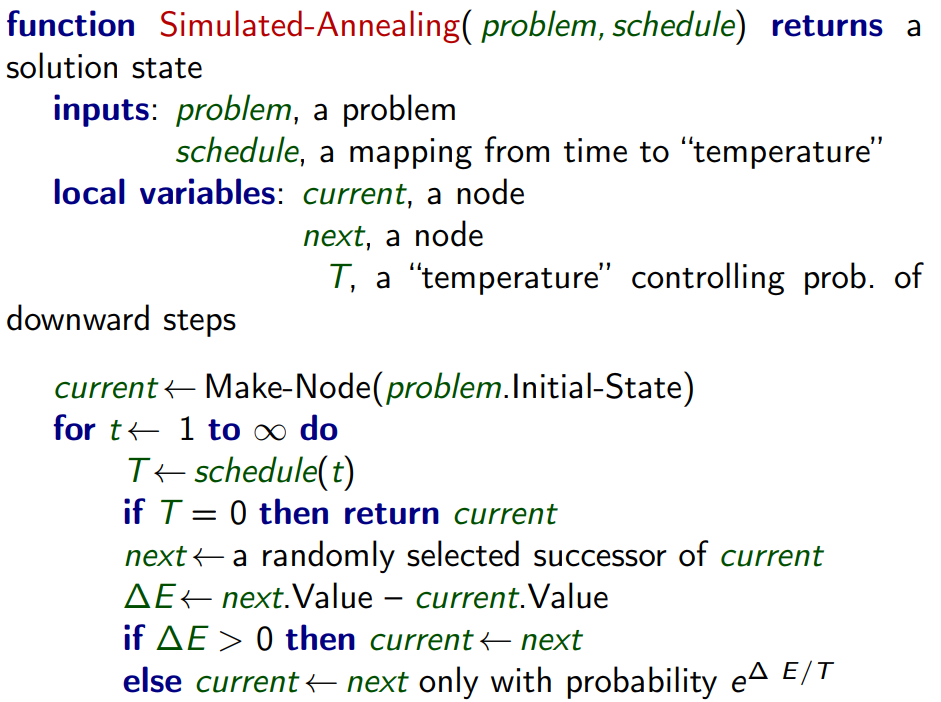
\includegraphics[width=\textwidth, height=\textheight, keepaspectratio]{simulated-annealing.png}
		\caption{Algoritmo simulated annealing}
	\end{subfigure}
	\hfill
	\begin{subfigure}{0.49\textwidth}
	    \centering
		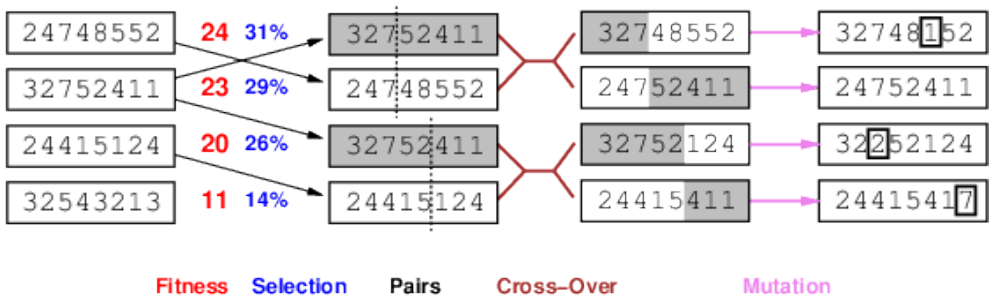
\includegraphics[width=\textwidth, height=\textheight, keepaspectratio]{genetic.png}
		\caption{Algoritmo genetico sul problema delle 8 regine}
	\end{subfigure}
\end{figure}

\section{Ricerca locale in spazi continui}
Si possono usare diversi metodi di ricerca locale anche per risolvere problemi negli \textit{spazi continui}. In particolare, i problemi di programmazione lineare e di ottimizzazione convessa obbediscono a determinati vincoli sulla forma dello spazio degli stati e sulla natura della \textit{funzione obiettivo}, e ammettono algoritmi con complessità temporale polinomiale che spesso sono estremamente efficienti nella pratica.


\chapter{Problemi di soddisfacimento di vincoli}

\section{Definizione dei problemi di soddisfacimento di vincoli}
Consideriamo come principale categoria di problemi risolvibili tramite reti a vincoli i \textit{problemi combinatori}, ovvero quei problemi in cui si deve scegliere la soluzione migliore tra le tante possibili. I problemi combinatori includono i problemi di \textit{decisione} e di \textit{ottimizzazione}.
\begin{figure}[htp]
	\centering
	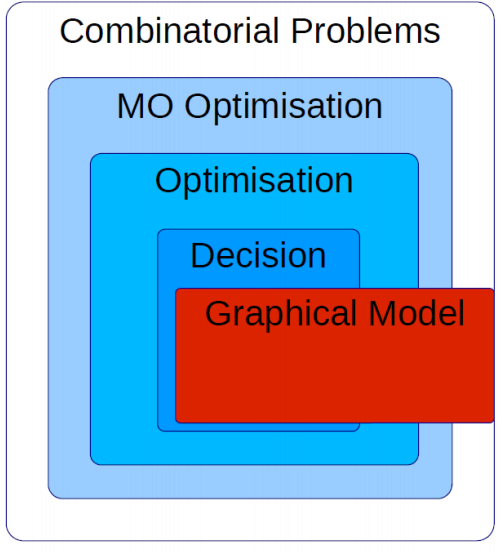
\includegraphics[width=0.35\textwidth]{csp.png}
\end{figure}

\subsection{Reti a vincoli}
Una \textit{rete a vincoli} è costituita da tre componenti:
\begin{itemize}
	\item Un insieme di \textit{variabili} $X = \{ x_1, ..., x_n \}$.
	\item Un insieme di \textit{domini} $D = \{ D_1, ..., D_n \}$ (uno per ogni variabile).
	\item Un insieme di \textit{vincoli} $C = \{ (S_1, R_1), ..., (S_m, R_m) \}$ che specificano le combinazioni di valori ammesse.
\end{itemize}
Si noti che un \textit{vincolo} è una coppia $(S_i, R_i)$ dove $S_i$ è una o più variabili ($S_i \subseteq X$) e $R_i$ è un sottoinsieme del prodotto cartesiano delle variabili in $S_i$.

La \textit{soluzione} di una rete a vincoli consiste nell'assegnamento dei valori ad alcune o a tutte le variabili in modo che i vincoli vengano soddisfatti (assegnamento \textit{consistente}). Un assegnamento è \textit{completo} se a tutte le variabili viene assegnato un valore, mentre è \textit{parziale} se menziona solo alcune delle variabili (un assegnamento parziale e consistente potrebbe non fare parte della soluzione).

\subsection{Un problema di esempio: colorazione di una mappa}
Il problema del \textit{map colouring} consiste nel fare in modo che in una mappa ogni regione abbia un colore diverso dalle regioni adiacenti. Supponendo di avere 5 regioni ($x_1, ..., x_5$), il \textit{grafo} dei vincoli si costruisce collegando tra loro con un arco le regioni che non devono avere lo stesso colore. Per sapere quali sono bisogna guardare ai \textit{vincoli}, i quali avranno una forma del tipo $C_k = (\{ x_i, x_j \}, x_i \neq x_j)$. Il grafo dei vincoli può essere rappresentato anche tramite:
\begin{itemize}
    \item \textit{Grafo primale}, il quale ha come nodi le variabili e come archi i vincoli.
    \item \textit{Grafo duale}, il quale ha come nodi i vincoli e come archi le variabili comuni ai vincoli collegati.
\end{itemize}
\begin{figure}[htp]
	\begin{subfigure}{0.49\textwidth}
	    \centering
		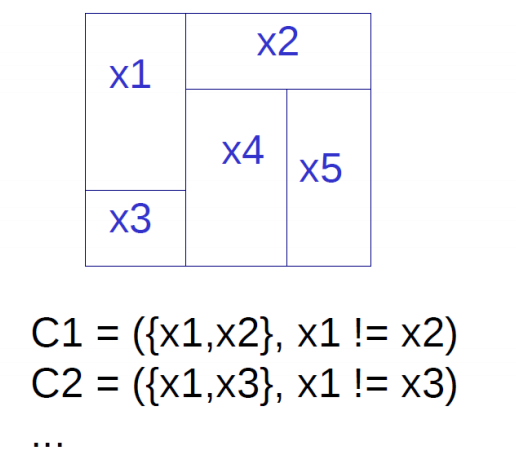
\includegraphics[width=0.95\textwidth]{map-col1.png} 
		\caption{Grafo dei vincoli}
	\end{subfigure}
	\hfill
	\begin{subfigure}{0.49\textwidth}
	    \centering
		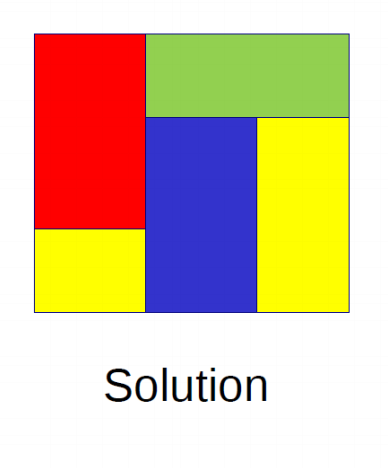
\includegraphics[width=0.75\textwidth]{map-col2.png} 
		\caption{Soluzione}
	\end{subfigure}
	\begin{subfigure}{0.49\textwidth}
	    \centering
		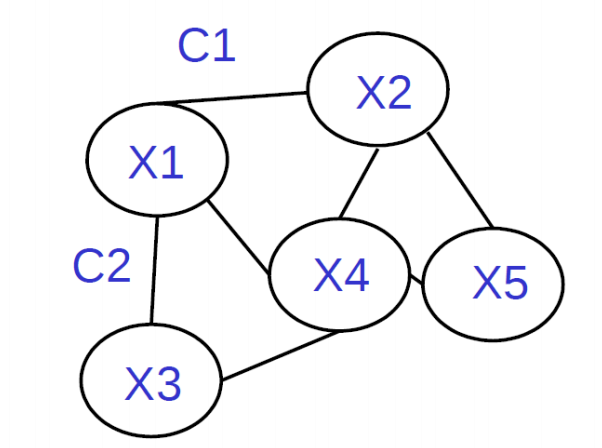
\includegraphics[width=0.85\textwidth]{primal.png}
		\caption{Grafo primale}
	\end{subfigure}
	\hfill
	\begin{subfigure}{0.49\textwidth}
	    \centering
		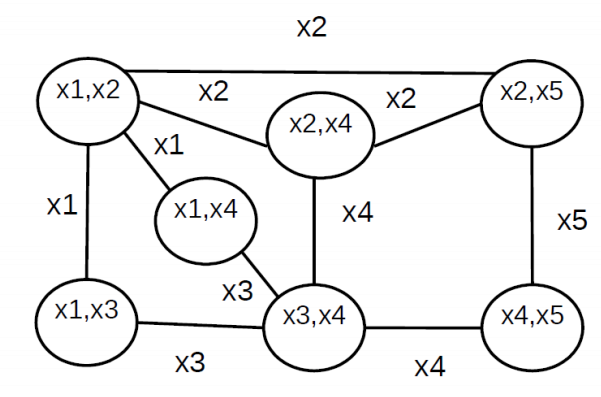
\includegraphics[width=0.95\textwidth]{dual.png}
		\caption{Grafo duale}
	\end{subfigure}
\end{figure}


\section{Tecniche risolutive per le reti a vincoli}
Le tecniche risolutive per le reti a vincoli più utilizzate sono quelle basate su:
\begin{itemize}
	\item \textit{Inferenza}, cioè quelle che generano nuovi vincoli a partire da quelli già esistenti.
	\item \textit{Ricerca}, cioè quelle che cercano la soluzione per tentativi.
\end{itemize}

\subsection{Ricerca con backtracking}
La \textit{ricerca con backtracking} è una forma particolare di ricerca in profondità in cui l'idea è quella di scegliere una variabile e aggiungere un nuovo vincolo su quella variabile per tentare di risolvere il resto del problema. Tuttavia, l'assegnamento parziale di una variabile può violare altri vincoli del problema e quindi è proprio qui che si fa \textit{backtracking} per tornare alla situazione precedente e procedere per un'altra via.

\subsection{Inferenza e propagazione dei vincoli}
Molte tecniche di \textit{inferenza} utilizzano i vincoli per inferire quali coppie valore/variabile sono consistenti e quali no allo scopo di generare reti più forti con uno spazio di ricerca più piccolo e quindi di migliorare prestazionalmente la ricerca della soluzione. Infatti, grazie alla \textit{propagazione} di nuovi vincoli è possibile ridurre lo spazio dei valori accettabili da una variabile, che a sua volta ridurrà lo spazio di un'altra variabile e così via.

\subsection{Metodi di consistenza}
Un'approssimazione dell'inferenza si può ottenere utilizzando i metodi di \textit{consistenza}. Gli approcci possibili sono: consistenza di \textit{nodo}, consistenza di \textit{arco}, consistenza di \textit{cammino} e \textit{i}-consistenza.

\paragraph{Consistenza di nodo.}
Una variabile $x_i$ del dominio $D_i$ è \textit{node consistent} se ogni suo valore all'interno del dominio soddisfa ogni vincolo unario.
\[ \forall v \in D_i. \, \forall C = \{ <x_i>, R_{x_i} \}. \, v \in R_{x_i} \]
In generale, se una variabile non è \textit{node consistent}, si possono rimuovere tutti i suoi valori nel dominio che non soddisfano tutti i vincoli unari per quella variabile. Il nuovo dominio della variabile diventerà un dominio che conterrà solo valori che soddisfano tutti i vincoli unari, e quindi quelli esclusi non potranno far parte della soluzione.
\[ D^{'}_i = D_i \setminus \{ v \, | \, \exists C = \{ <x_i>, R_{x_i} \} \wedge v \notin R_{x_i}  \} \]

\paragraph{Consistenza di arco.}
Date due variabili $x_i$ e $x_j$, $x_i$ è \textit{arc consistent} rispetto a $x_j$ se vale che:
\[ \forall a_i \in D_i. \, \exists a_j \in D_j. \, (a_i, a_j) \in R_{x_i, x_j} \]
Da questo si conclude che $R_{x_i, x_j}$ è \textit{arc consistent} se $x_i$ è \textit{arc consistent} rispetto a $x_j$ e viceversa. Il nuovo dominio conterrà solo valori che soddisfano i vincoli binari, e quindi quelli esclusi non potranno far parte della soluzione.

Per verificare l'\textit{arc consistency} si possono utilizzare gli algoritmi \textit{AC-1} e \textit{AC-3}. Tali algoritmi fanno uso della procedura di \textit{Revise}, ovvero della rimozione dei valori in un dominio per i quali non vale l'\textit{arc consistency} rispetto ad un secondo dominio. L'algoritmo \textit{AC-1} ha complessità $O(nek^3)$ dove $n$ sono i nodi, $e$ sono gli archi e $k$ è il massimo numero di valori in un dominio.  Inoltre, \textit{AC-1} termina sempre e mantiene l'\textit{arc consistency}, tranne se la rete è vuota in quanto non esisterà alcuna soluzione. L'algoritmo \textit{AC-3}, invece, è un miglioramento di \textit{AC-1} con complessità $O(ek^3)$.
\begin{figure}[htp]
	\begin{subfigure}{0.49\textwidth}
	    \centering
		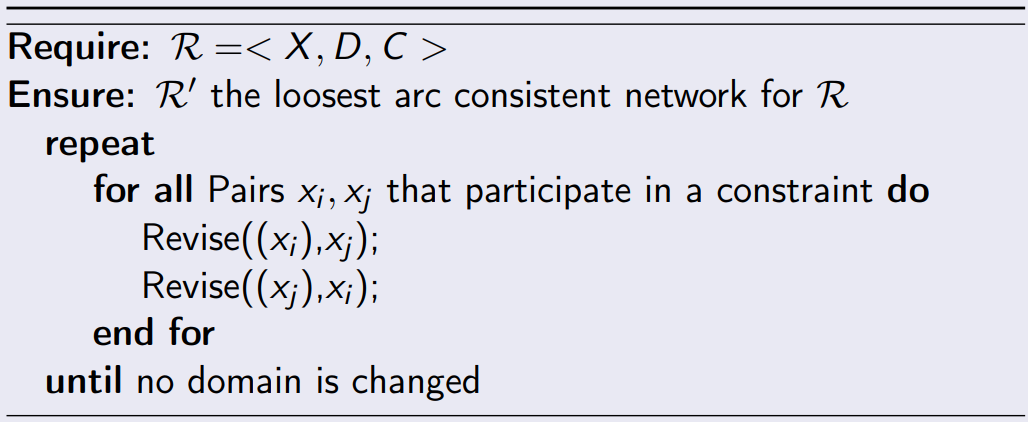
\includegraphics[width=\textwidth, height=\textheight, keepaspectratio]{ac-1.png}
		\caption{Algoritmo AC-1}
	\end{subfigure}
	\hfill
	\begin{subfigure}{0.49\textwidth}
	    \centering
		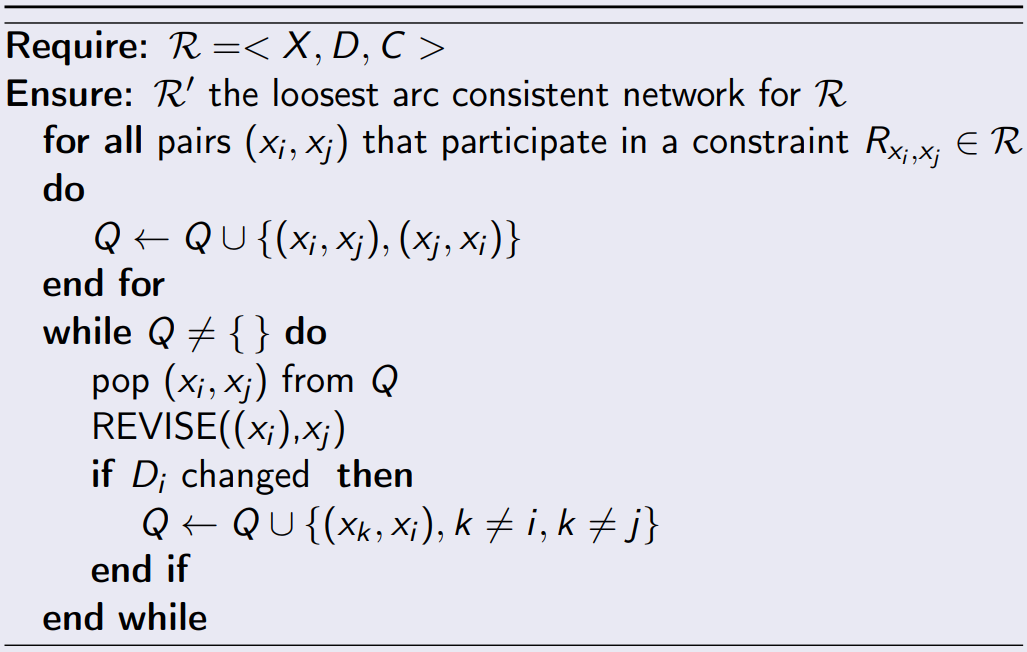
\includegraphics[width=\textwidth, height=\textheight, keepaspectratio]{ac-3.png}
		\caption{Algoritmo AC-3}
	\end{subfigure}
\end{figure}

Abbiamo detto che se un dominio è vuoto, allora si ha un problema inconsistente (non esiste alcuna soluzione). Al contrario, se tutti i domini sono non vuoti \textit{non implica} che il problema è consistente. Infatti, il principale punto debole dell'\textit{arc consistency} è che lavora solamente su vincoli binari e su vincoli con un singolo dominio.

\paragraph{Consistenza di cammino.}
\`{E} un'evoluzione della consistenza di arco che restringe i vincoli binari utilizzando vincoli impliciti che sono inferiti considerando \textit{triplette di variabili}.

\paragraph{i-consistenza.}
La \textit{i-consistenza} è un'estensione del concetto della consistenza di arco (e della consistenza di cammino) a reti di $i-1$ variabili. Diciamo che una rete è \textit{i-consistent} se, per ogni insieme di $i-1$ variabili e ogni loro assegnamento consistente, è sempre possibile assegnare un valore consistente a ogni \textit{i}-esima variabile. Inoltre, diciamo che una rete è \textit{fortemente i-consistente} se è anche \textit{j}-consistente per ogni $j \leq i$.


\section{Strategie di ricerca per la propagazione dei vincoli}
Una strategia di ricerca \textit{standard} può consistere nell'applicare la ricerca a profondità limitata. In questo caso, uno stato sarebbe un assegnamento parziale e un'azione sarebbe l'aggiunta di $variabile = valore$ all'assegnamento. Tuttavia, per un problema di soddisfacimento di vincoli (\textit{CSP}) con $n$ variabili con dominio di dimensione $d$ si può notare che il fattore di ramificazione al livello $l$ è pari a $b = (n - l) d$, e quindi l'albero generato avrebbe $n! \cdot d^n$ foglie.

La formulazione del problema precedente è apparentemente ragionevole, ma in realtà è \textit{ingenua} in quanto ha ignorato una proprietà fondamentale comune a tutti i \textit{CSP}, ovvero la commutatività. Un problema è \textit{commutativo} se l'ordine di applicazione di un qualsiasi insieme di azioni non ha effetto sul risultato finale.

\subsection{Backtracking search}
I \textit{CSP} sono commutativi perché assegnando valori alle variabili si ottiene sempre lo stesso assegnamento parziale indipendentemente dall'ordine degli assegnamenti. Di conseguenza ci basta considerare \textit{una sola} variabile in ogni livello dell'albero di ricerca. Con questa restrizione il numero di foglie risulterebbe pari a $d^n$. Indicheremo quindi con il termine \textit{backtracking search} una ricerca in profondità che assegna valori a una variabile per volta e torna indietro quando non ci sono più valori legali da assegnare.
\begin{figure}[htp]
	\begin{subfigure}{0.49\textwidth}
	    \centering
		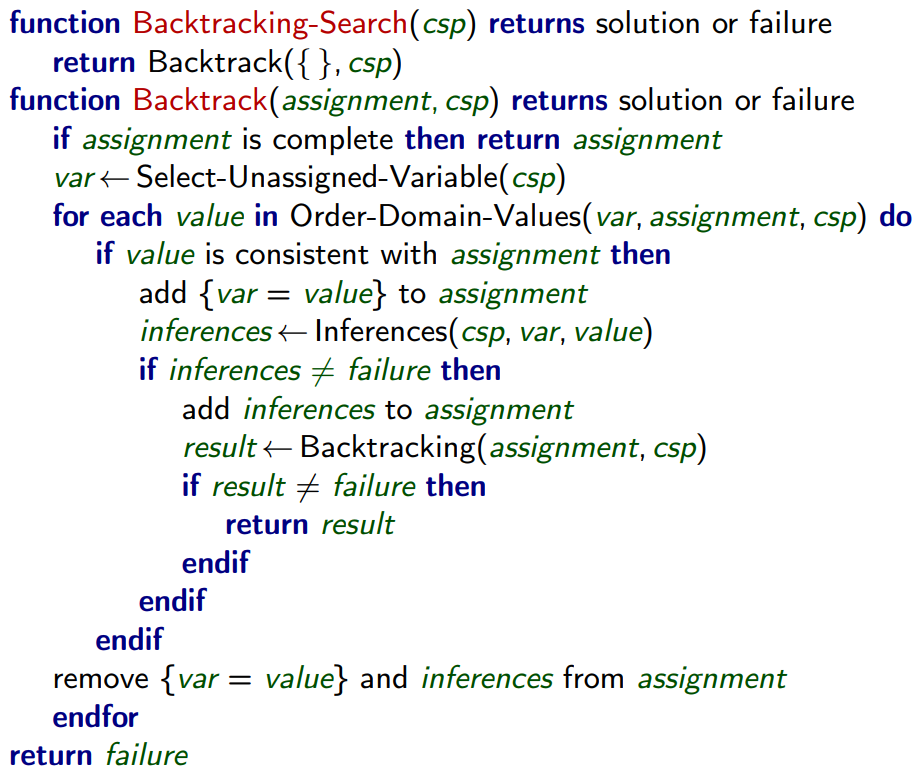
\includegraphics[width=\textwidth, height=\textheight, keepaspectratio]{backtracking-search.png}
		\caption{Algoritmo backtracking search}
	\end{subfigure}
	\hfill
	\begin{subfigure}{0.49\textwidth}
	    \centering
		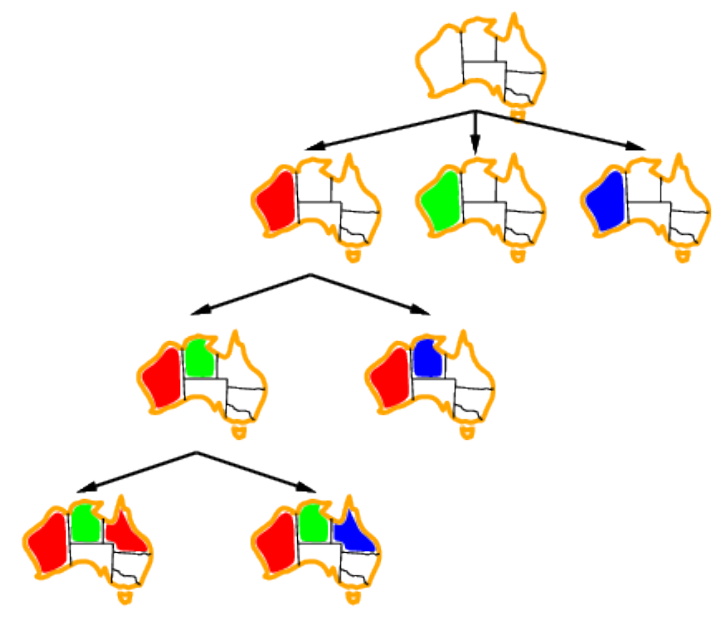
\includegraphics[width=\textwidth, height=\textheight, keepaspectratio]{backtracking-example.png}
		\caption{Albero di ricerca (parziale)}
	\end{subfigure}
\end{figure}

\subsection{Ordinamento di variabili}
Per migliorare la \textit{backtracking search} possiamo cambiare la strategia per scegliere la variabile da assegnare nel passo successivo. La strategia più semplice è quella di scegliere la prima variabile non assegnata, ma tale ordinamento statico raramente dà come risultato la ricerca più efficiente. L'idea è quindi quella di scegliere la variabile con il minor numero di valori legali. Tale euristica è chiamata \textit{MRV} (Minimum Remaining Values) perché sceglie appunto la variabile per cui è maggiore la probabilità di arrivare presto ad un fallimento (variabile più vincolata). Tuttavia, l'euristica \textit{MRV} non è di alcun aiuto nella scelta della prima regione da colorare, perché all'inizio ognuna di esse ha esattamente tre colori legali. In questo caso viene in aiuto l'euristica \textit{DH} (Degree Heuristic), la quale cerca di ridurre il fattore di ramificazione delle scelte future scegliendo la variabile coinvolta nel maggior numero di vincoli con le altre variabili non assegnate.
\begin{figure}[htp]
	\begin{subfigure}{0.49\textwidth}
	    \centering
		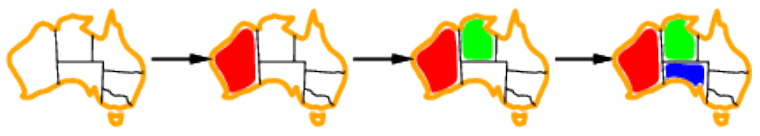
\includegraphics[width=\textwidth, height=\textheight, keepaspectratio]{mrv.png}
		\caption{Euristica MRV}
	\end{subfigure}
	\hfill
	\begin{subfigure}{0.49\textwidth}
	    \centering
		
\includegraphics[width=\textwidth, height=\textheight, keepaspectratio]{dh.png}
		\caption{Euristica DH}
	\end{subfigure}
\end{figure}

\subsection{Ordinamento di valori}
Una volta scelta una variabile, l'algoritmo deve anche decidere l'ordine con cui esaminare i suoi possibili valori. Sempre per migliorare la \textit{backtracking search}, in alcuni casi può essere efficace l'euristica del \textit{valore meno vincolante}, la quale predilige il valore che lascia più libertà alle variabili adiacenti sul grafo dei vincoli. In generale, l'euristica cerca sempre di lasciare la massima flessibilità ai successivi assegnamenti di variabili.
\begin{figure}[htp]
	\centering
	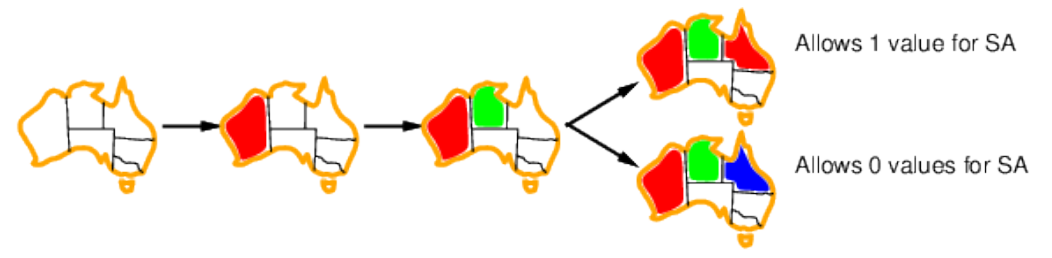
\includegraphics[width=\textwidth, height=\textheight, keepaspectratio]{lcv.png}
\end{figure}

\subsection{Alternanza di ricerca e inferenza}
Finora abbiamo visto come inferire riduzioni del dominio di variabili \textit{prima} di iniziare la ricerca, ma l'inferenza può risultare ancora più potente nel corso di una ricerca. Infatti, ogni volta che scegliamo un valore per una variabile, abbiamo un'opportunità del tutto nuova di inferire nuove riduzioni di dominio sulle variabili adiacenti. Una delle forme di inferenza più semplici è la cosiddetta verifica in avanti (\textit{forward checking}) in cui, ogni volta che una variabile $X$ viene assegnata, si stabilisce la \textit{consistenza di arco} per essa, ovvero per ogni variabile non assegnata $Y$ collegata a $X$ da un vincolo si cancella dal dominio di $Y$ ogni valore non consistente con quello scelto per $X$. La verifica in avanti rileva molte inconsistenze, ma non tutte. Il problema è che rende la variabile corrente \textit{arc consistent}, ma non guarda avanti per rendere \textit{arc consistent} tutte le altre.
\begin{figure}[htp]
	\centering
	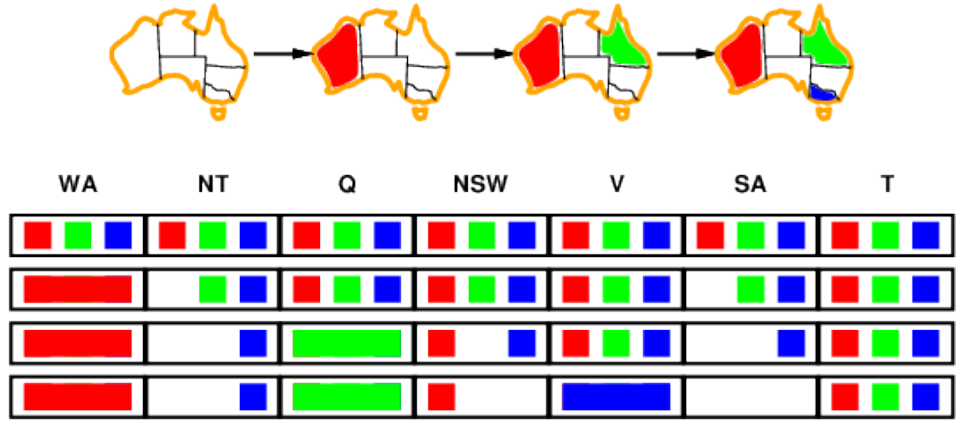
\includegraphics[width=\textwidth, height=\textheight, keepaspectratio]{forward-checking.png}
\end{figure}

\subsection{Mantaining Arc Consistency}
L'algoritmo \textit{MAC} (Mantaining Arc Consistency) rileva le inconsistenze che la verifica in avanti non riesce a rilevare. Infatti, \textit{MAC} è strettamente più potente della verifica in avanti perché quest'ultima procede come \textit{MAC} sugli archi iniziali nella coda di \textit{MAC}, ma non propaga ricorsivamente i vincoli quando si apportano modifiche ai domini delle variabili.


\section{La struttura dei problemi}
Per riuscire a trovare più rapidamente una soluzione, si può sfruttare la \textit{struttura} stessa del problema (rappresentata dal grafo dei vincoli). L'unico modo in cui possiamo sperare di gestire la complessità del mondo reale è scomporlo in molti sotto-problemi. Infatti, se riuscissimo a scomporre il grafo dei vincoli fino a farlo diventare un albero, potremmo risolvere il \textit{CSP} in un tempo che cresce linearmente con il numero delle variabili. Un grafo dei vincoli è un \textit{albero} quando due variabili qualsiasi sono collegate da un solo cammino. Per \textit{ridurre} un grafo dei vincoli ad un albero si può utilizzare un approccio, basato sulla rimozione dei nodi, che prevede che si assegnino dei valori ad alcune variabili in modo che quelle rimanenti formino un albero. L'algoritmo generale di questo approccio è il seguente:
\begin{enumerate}
    \item Scegliere un sottoinsieme $S$ delle variabili del \textit{CSP} tale che il grafo dei vincoli diventi un albero dopo la rimozione di $S$ (\textit{cycle cutset}).
    \item Per ogni possibile assegnamento delle variabili in $S$ che soddisfa tutti i vincoli su $S$:
    \begin{enumerate}
        \item Rimuovere dal dominio delle variabili rimanenti tutti i valori non consistenti con gli assegnamenti in $S$.
        \item Se il \textit{CSP} risultante ha una soluzione, restituirla insieme all'assegnamento per $S$.
    \end{enumerate}
\end{enumerate}
Se il \textit{cycle cutset} $S$ ha dimensione $c$, il tempo di esecuzione totale è $O(d^c \cdot (n-c)d^2)$. Se il grafo è quasi un albero $c$ sarà piccolo, e il risparmio di tempo rispetto al backtracking risulterà enorme.
\begin{figure}[htp]
	\centering
	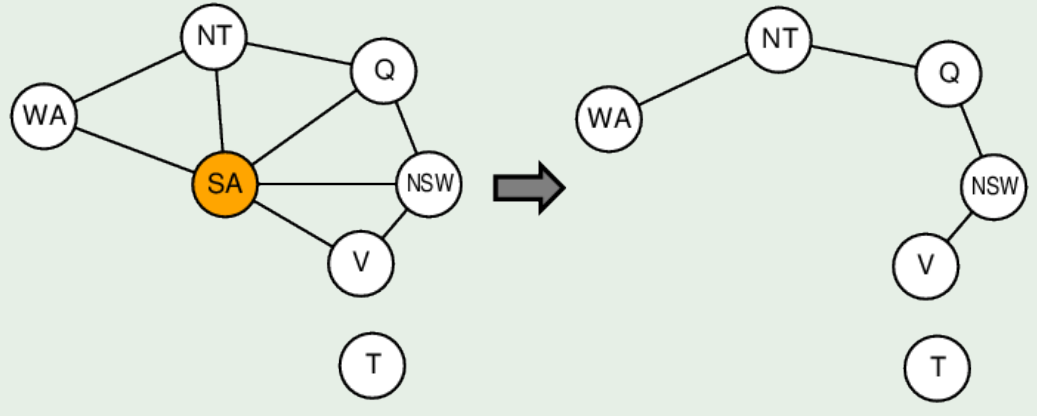
\includegraphics[width=\textwidth, height=\textheight, keepaspectratio]{cycle-cutset.png}
\end{figure}

\subsection{Scomposizione ad albero}
Un processo alternativo per ridurre un grafo dei vincoli ad un albero è quello basato sulla costruzione di una scomposizione ad albero (\textit{tree decomposition}) del grafo dei vincoli in un insieme di sotto-problemi collegati. Secondo questo approccio, poi, ogni sotto-problema viene risolto indipendentemente e le soluzioni vengono combinate insieme. Il processo di tree decomposition viene quindi applicato quando si vuole passare da reti cicliche a \textit{reti acicliche}, in quanto l'inferenza su queste ultime è molto più efficiente.

\subsection{Concetto di ipergrafo}
Un \textit{ipergrafo} è una struttura $H = (V, S)$ dove $V$ è un insieme di nodi e $S$ è un insieme di iperarchi ossia un insieme $S = \{ S_1, ..., S_k \}$ tale che $S_i \subseteq V$. Il \textit{grafo primale} di un ipergrafo sarà quindi un grafo in cui: i nodi sono i vertici; due nodi vengono collegati da un arco solo se appaiono nello stesso iperarco. Il \textit{grafo duale} di un ipergrafo, invece, sarà un grafo in cui: i nodi sono gli iperarchi; due nodi vengono collegati da un arco solo se condividono almeno un vertice (gli archi verranno quindi etichettati con i vertici condivisi tra i nodi).

\subsection{Rappresentazione di una rete a vincoli}
Ogni rete a vincoli può essere rappresentata tramite un ipergrafo. Infatti, per la rete a vincoli $\mathcal{R} = \{ X, D, C \}$ con $C = \{ R_{S_1}, ..., R_{S_r} \}$ il relativo ipergrafo è $\mathcal{H}_\mathcal{R} = (X,H)$ con $H = \{ S_1, ..., S_r \}$. Inoltre, il grafo duale è $\mathcal{H}_\mathcal{R}^d = (H,E)$ con $<S_i, S_j> \in E \iff S_i \cap S_j \neq \{ \}$.

\subsection{Reti acicliche}
I concetti principali relativi alle reti acicliche sono i seguenti.
\begin{itemize}
    \item \textit{Sottografo}: si definisce sottografo di un grafo $G=(V,E)$ il grafo $G' = (V, E')$ tale per cui $E' \subseteq E$.
    \item \textit{Running intersection property}: dato il grafo duale $G$ di un ipergrafo, il suo sottografo $G'$ soddisfa la running intersection property se, tra due nodi qualsiasi di $G'$ che condividono una variabile, esiste un percorso formato da archi etichettati almeno con la variabile condivisa.
    \item \textit{Join-graph}: si definisce join-graph un sottografo $G'$, di un grafo duale $G$ di un ipergrafo, che soddisfa la running intersection property.
    \item \textit{Join-tree}: si definisce join-tree un join-graph aciclico.
    \item \textit{Iperalbero}: si definisce iperalbero un ipergrafo il cui grafo duale ha un join-tree.
\end{itemize}
Una \textit{rete aciclica} viene quindi definita come una rete il cui ipergrafo è un iperalbero.

\subsection{Risolvere una rete aciclica}
Per risolvere una rete aciclica è sufficiente risolvere l'albero mediante l'\textit{algoritmo Tree Solver}. Tuttavia, è necessario prima sapere come fare a determinare se una rete è aciclica. I principali metodi per eseguire questa verifica sono la dual-based e la primal-based recognition.

L'idea alla base della \textit{dual-based recognition} è che se un ipergrafo ammette un join-tree, allora ogni maximum spanning tree del suo grafo duale è un join-tree. La \textit{procedura} da applicare è quindi la seguente:
\begin{itemize}
	\item Costruire il grafo duale dell'ipergrafo.
	\item Determinare un maximum spanning tree usando come peso il numero delle variabili condivise.
	\item Controllare se l'iperalbero è un join-tree.
\end{itemize}

L'idea alla base della \textit{primal-based recognition}, invece, è che un ipergrafo ammette un join-tree se valogono le proprietà di:
\begin{itemize}
    \item \textit{Cordalità}, per cui un grafo primale si dice cordale se ogni ciclo di lunghezza almeno pari a 4 ha una corda (ovvero un arco che collega due vertici non adiacenti in un ciclo).
    \item \textit{Conformalità}, per cui un grafo primale si dice conformale ad un ipergrafo se esiste una corrispondenza uno a uno tra clique massimali e scope dei vincoli.
\end{itemize}
La verifica di queste due proprietà viene eseguita in maniera efficiente se viene usato un \textit{ordine di massima cardinalità}. La \textit{procedura} da applicare è quindi la seguente:
\begin{itemize}
	\item Costruire un ordine di massima cardinalità.
	\item Testare se il grafo è cordale, ovvero se nell'ordine di massima cardinalità ogni vertice e i suoi predecessori formano una clique.
	\item Testare se il grafo è conformale estraendo la clique massimale.
\end{itemize}
\begin{figure}[htp]
	\begin{subfigure}{0.3\textwidth}
        \centering
        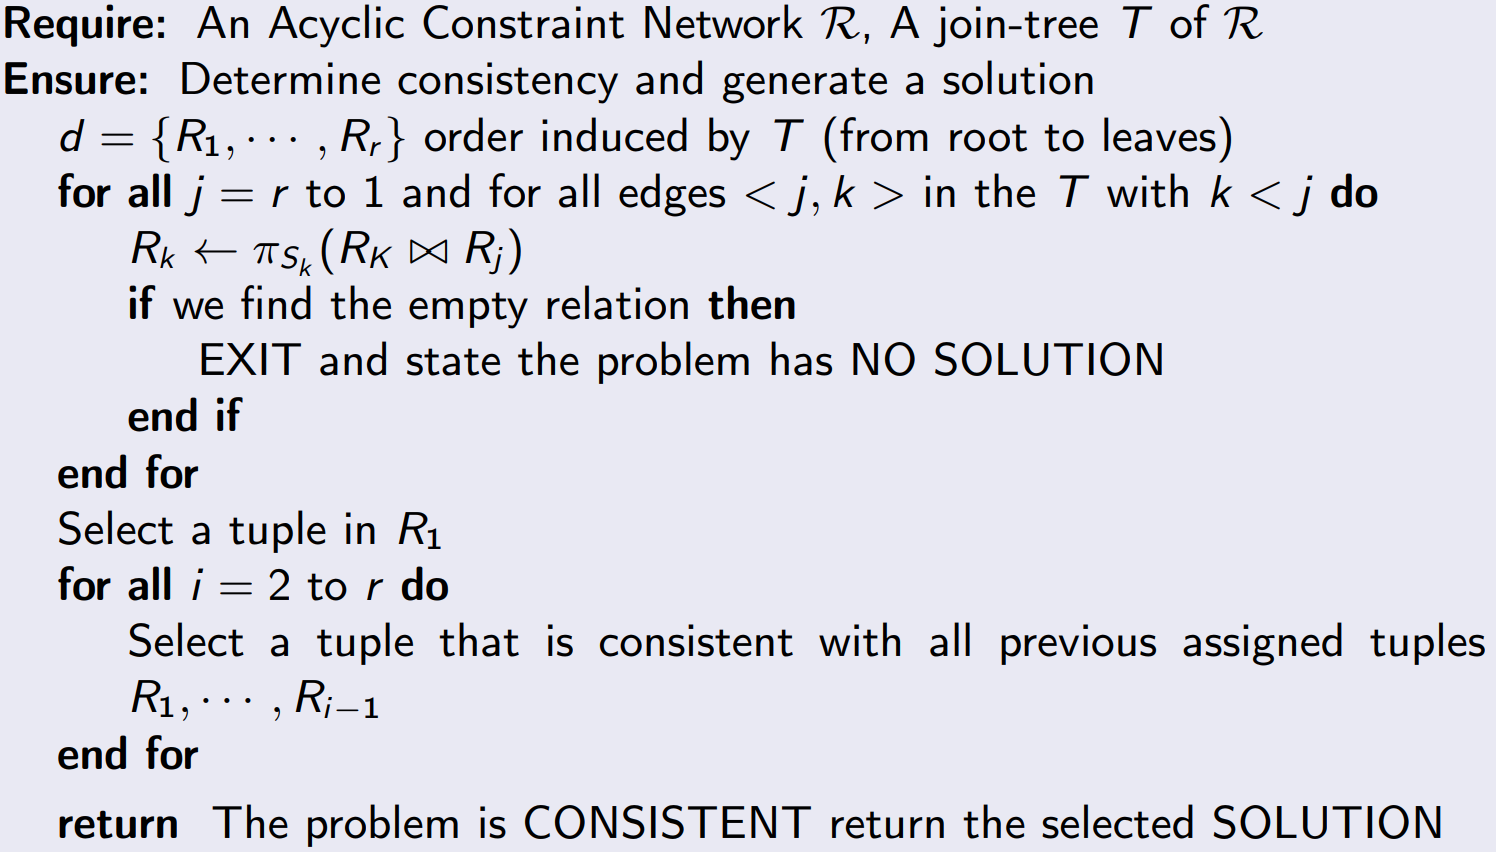
\includegraphics[width=\textwidth, height=\textheight, keepaspectratio]{tree-solver.png}
        \caption{Algoritmo Tree Solver}
    \end{subfigure}
    \hfill
    \begin{subfigure}{0.3\textwidth}
        \centering
        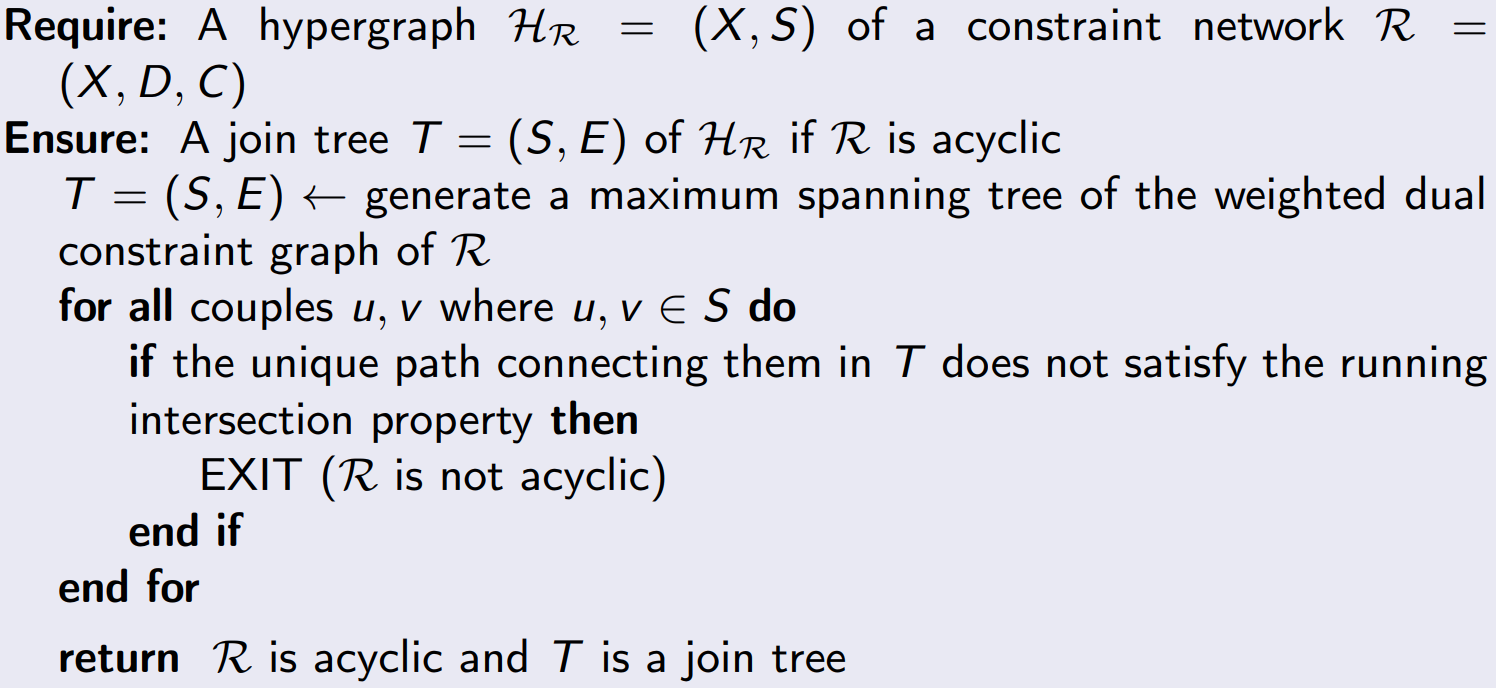
\includegraphics[width=\textwidth, height=\textheight, keepaspectratio]{dual-acyclicicty.png}
        \caption{Algoritmo DualAcyclicicty}
    \end{subfigure}
    \hfill
    \begin{subfigure}{0.3\textwidth}
        \centering
        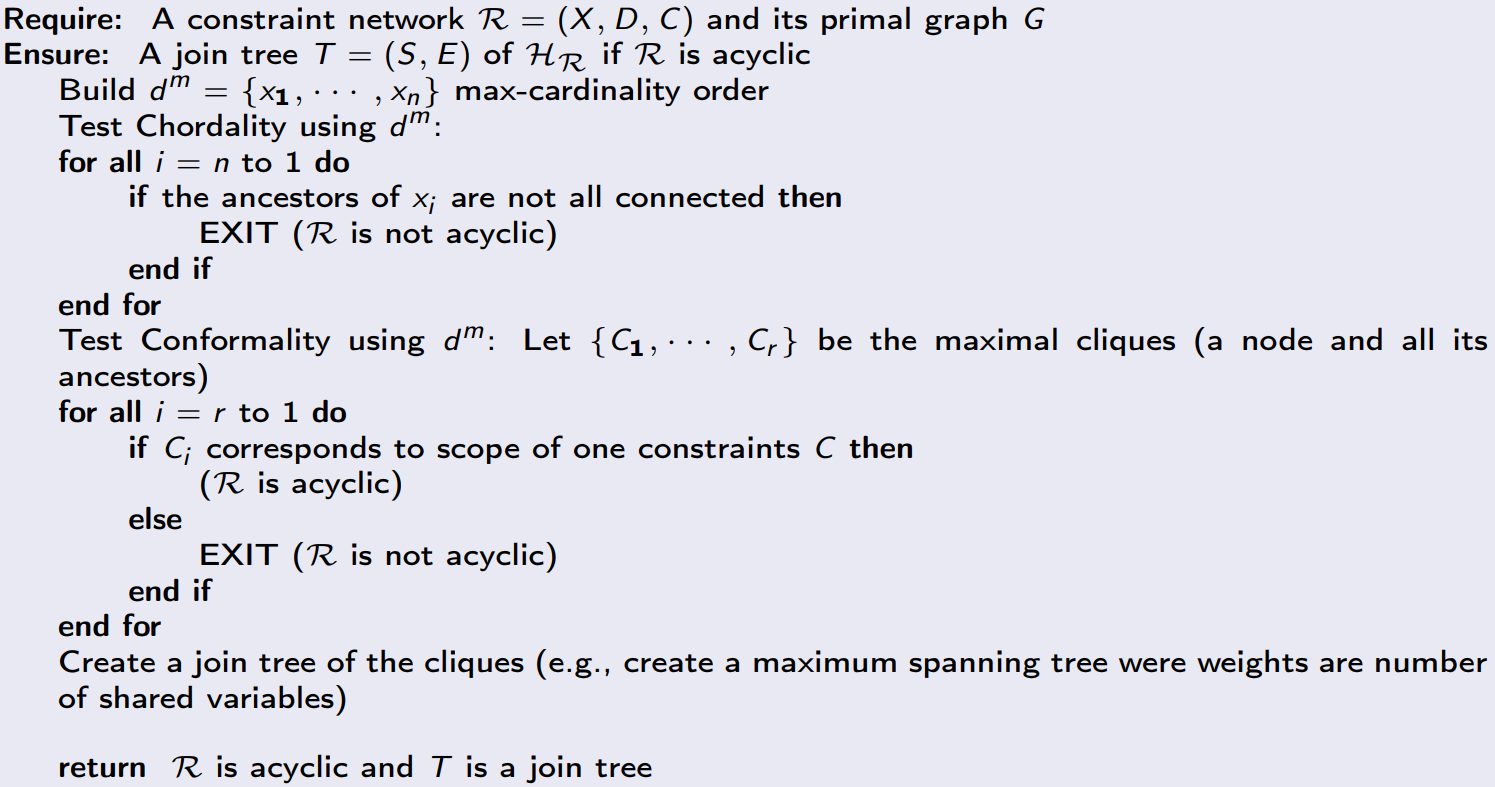
\includegraphics[width=\textwidth, height=\textheight, keepaspectratio]{primal-acyclicicty.png}
        \caption{Algoritmo PrimalAcyclicicty}
    \end{subfigure}
\end{figure}

\subsection{Clustering}
La procedura del \textit{clustering} consiste nell'accorpare vincoli per ottenere una struttura ad albero e cercare quindi di risolvere in maniera più efficiente la rete. L'approccio più utilizzato è il cosiddetto \textit{join-tree clustering}, in cui per generare un join-tree si usa il seguente metodo:
\begin{enumerate}
	\item Si sceglie un ordine delle variabili.
	\item Si crea un grafo indotto per il quale valga la running intersection property:
	\begin{itemize}
	    \item Calcolando gli antenati di ogni variabile (processandole dall'ultima alla prima).
	    \item Verificando che ogni variabile formi una clique.
	\end{itemize}
	\newpage
	\item Si crea un join-tree:
	\begin{itemize}
		\item Identificando tutte le clique massimali $C_1, ..., C_t$ nel grafo indotto.
		\item Creando una struttura ad albero con le clique (ovvero un maximum spanning tree dove i pesi rappresentano il numero delle variabili condivise).
	\end{itemize}
	\item Si allocano i vincoli ad ogni clique che contiene il relativo scope (sotto-problema $P_i$ associato a $C_i$).
	\item Si risolve ogni sotto-problema $P_i$ ricavando il relativo insieme di soluzioni $R_i'$.
	\item Si determina la soluzione globale $C' = \{ R_1', ..., R_t' \} $ applicando l'algoritmo Tree Solver.
\end{enumerate}
La \textit{complessità} del join-tree clustering è dominata dal calcolo dell'insieme di soluzioni di ogni sotto-problema, il quale è esponenziale nella dimensione della clique. L'ordine delle variabili usato per calcolare le clique è quindi fondamentale, ma trovare l'ordine migliore è estremamente difficile.


\section{Constraint optimisation problems}
Per risolvere un \textit{COP} (constraint optimisation problem) si può ricorrere alle reti di costo. Si parla di reti di costo (\textit{cost network}) quando si ha a che fare con massimizzazioni o minimizzazioni di funzioni di costo. Infatti, una rete di costo è una rete a vincoli con una \textit{funzione di costo} applicata su di essa e definita come $F(\bar{a}) = \sum_{j=1}^l F_j(\bar{a})$ dove $\bar{a} = \{ a_1, ..., a_n \}$ sono gli assegnamenti delle variabili $X = \{ x_1, ..., x_n \}$. Lo scopo sarà quindi quello di trovare un'allocazione $\bar{a}^\ast$ di tali variabili che massimizzi o minimizzi la funzione di costo, ovvero $\bar{a}^\ast= max_{\bar{a}} F(\bar{a})$ oppure $\bar{a}^\ast = min_{\bar{a}} F(\bar{a})$.

\subsection{Metodi risolutivi per le reti di costo}
Le reti di costo si possono risolvere tramite:
\begin{itemize}
	\item \textit{Branch and Bound}, ovvero tramite un approccio simile alla ricerca con backtracking.
	\item \textit{Programmazione dinamica}, ovvero tramite approcci di inferenza.
\end{itemize}

\subsection{Branch and Bound}
Si ricorda che l'idea di base del \textit{backtracking} è quella di trovare progressivamente la soluzione migliore sulla base di una soluzione parziale, e di sfruttare tale soluzione parziale per il taglio (pruning) dell'albero di ricerca. Se per risolvere un COP dobbiamo, ad esempio, massimizzare una funzione di costo allora dovremo mantenere un \textit{lower bound} per riuscire a tagliare l'albero di ricerca. Infatti, vogliamo che tutte le soluzioni minori del lower bound siano scartate, in quanto non ha senso proseguire lungo un valore che è minore di quello massimo trovato finora.

\subsection{Bucket Elimination}
L'idea di base della \textit{programmazione dinamica} è quella di costruire la soluzione di un problema in modo incrementale partendo dalle soluzioni dei suoi sotto-problemi (si sfrutta la struttura del problema). L'algoritmo di \textit{Bucket Elimination} è una tecnica specifica di programmazione dinamica usata per risolvere i COP.
\newpage
I concetti alla base dell'algoritmo sono i seguenti passaggi.
\begin{enumerate}
    \item \textit{Bucket partition}: si assegnano i vincoli al bucket, il quale non è altro che un insieme di vincoli che fanno riferimento ad una variabile.
    \item \textit{Bucket processing}: si processa il bucket dall'ultima variabile alla prima secondo un certo ordinamento delle variabili.
    \item \textit{Value propagation}: si calcola la tupla ottimale propagando i valori dalla prima variabile all'ultima.
\end{enumerate}
La \textit{complessità} dell'algoritmo di Bucket Elimination è influenzata dalla scelta dell'ordinamento delle variabili; infatti, essa è esponenziale nella dimensione del bucket più grande.
\begin{figure}[htp]
	\begin{subfigure}{0.49\textwidth}
	    \centering
		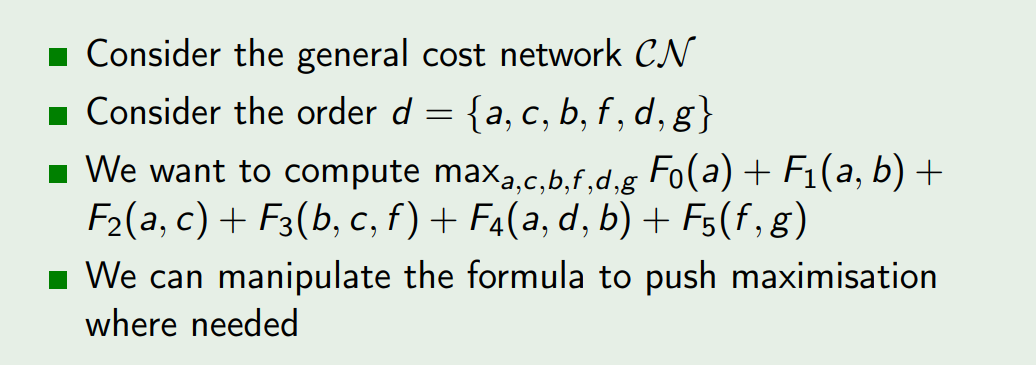
\includegraphics[width=\textwidth, height=\textheight, keepaspectratio]{dp-example1.png} 
		\caption{Bucket Elimination su una rete di costo}
	\end{subfigure}
	\hfill
	\begin{subfigure}{0.49\textwidth}
	    \centering
		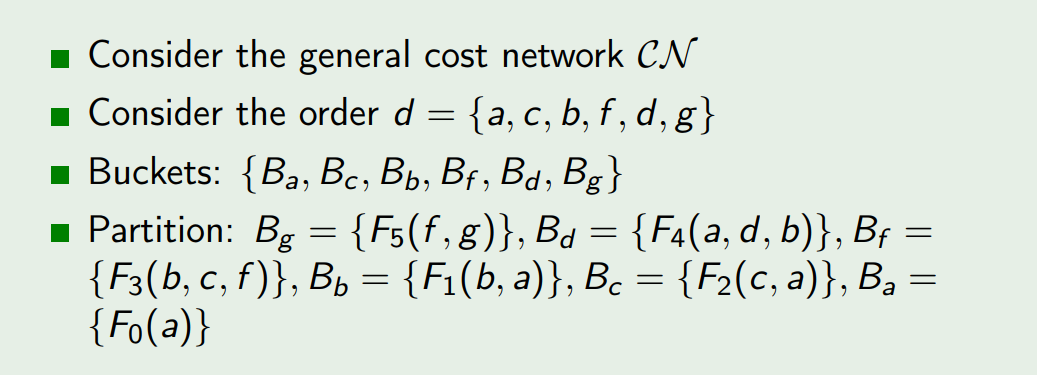
\includegraphics[width=\textwidth, height=\textheight, keepaspectratio]{dp-example2.png} 
		\caption{Bucket partition}
	\end{subfigure}
	\begin{subfigure}{0.49\textwidth}
	    \centering
		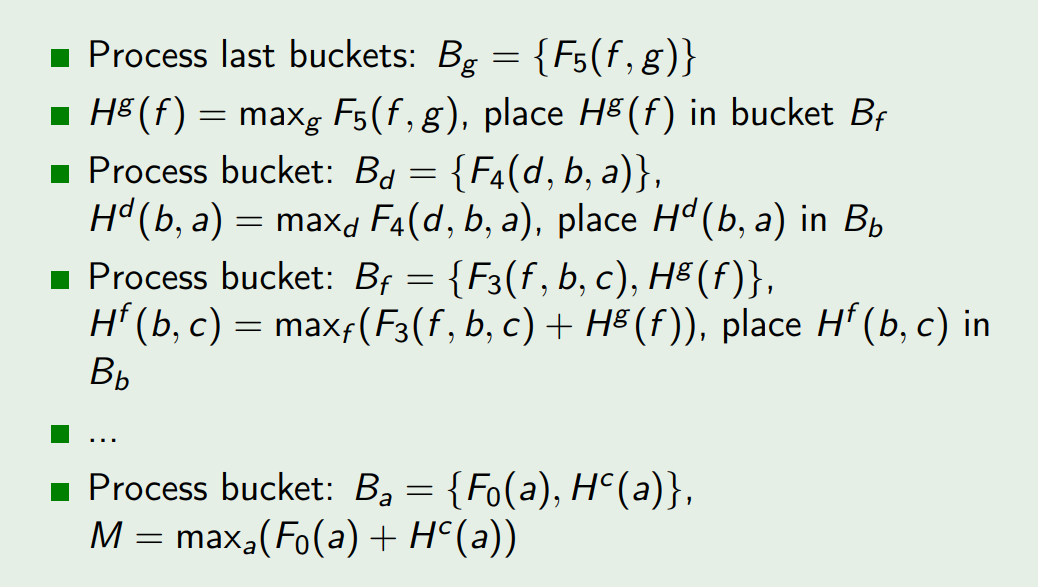
\includegraphics[width=\textwidth, height=\textheight, keepaspectratio]{dp-example3.png}
		\caption{Bucket processing}
	\end{subfigure}
	\hfill
	\begin{subfigure}{0.49\textwidth}
	    \centering
		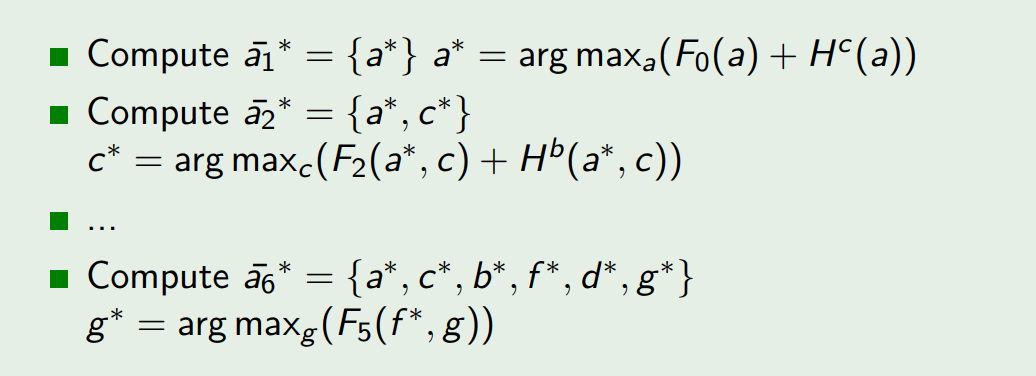
\includegraphics[width=\textwidth, height=\textheight, keepaspectratio]{dp-example4.png}
		\caption{Value propagation}
	\end{subfigure}
\end{figure}


\chapter{Incertezza}

\section{Agire in condizioni di incertezza}
La teoria della probabilità è il modo migliore di ragionare in condizioni di incertezza. Tale \textit{incertezza} può sorgere a causa di pigrizia e ignoranza, ed è infatti una caratteristica inevitabile dei mondi complessi, dinamici o non del tutto accessibili. La presenza di incertezza impedisce di effettuare molte delle semplificazioni possibili grazie all'inferenza deduttiva.

\section{Notazione base della teoria della probabilità}
Le \textit{probabilità} esprimono l'incapacità dell'agente di arrivare ad una decisione definitiva sul valore di verità di una formula e servono a riassumere le sue credenze. Gli enunciati base includono le probabilità a priori e le probabilità condizionate di proposizioni semplici e complesse.

\subsection{Probabilità a priori}
La \textit{probabilità a priori} (o non condizionata) associata con una proposizione $a$ è il grado di credenza che le viene accordato in assenza di ogni altra informazione; viene indicata con $P(a)$. Una \textit{distribuzione di probabilità} viene definita quando si considerano le probabilità di tutti i possibili valori di una variabile casuale. Se invece vogliamo denotare le probabilità di tutte le combinazioni di valori di un insieme di variabili casuali, allora definiremo una distribuzione di probabilità \textit{congiunta}.

\subsection{Probabilità condizionate}
Una volta che l'agente ha ottenuto delle prove precedentemente sconosciute riguardo alle variabili casuali del dominio, le probabilità a priori non sono più applicabili. Al posto di queste ultime si devono infatti usare le \textit{probabilità condizionate} (o a posteriori). La notazione è $P(a|b)$ (con $a$ e $b$ proposizioni qualsiasi) e indica la probabilità di $a$ posto che tutto quello che sappiamo è $b$. Infine, le probabilità condizionate possono essere definite partendo da quelle non condizionate:
\[ P(a|b) = \frac{P(a \wedge b)}{P(b)} \]
con $P(b) \neq 0$.

\section{Inferenza basata su distribuzioni congiunte complete}
La distribuzione di probabilità \textit{congiunta completa} specifica la probabilità di ogni assegnamento completo di valori alle variabili casuali. Quando tale distribuzione è disponibile, si può rispondere ad un'interrogazione semplicemente sommando le probabilità degli eventi atomici che corrispondono alle proposizioni della query. Solitamente però la distribuzione congiunta completa risulta troppo grande per essere creata o utilizzata in forma esplicita.
\begin{figure}[htp]
	\centering
	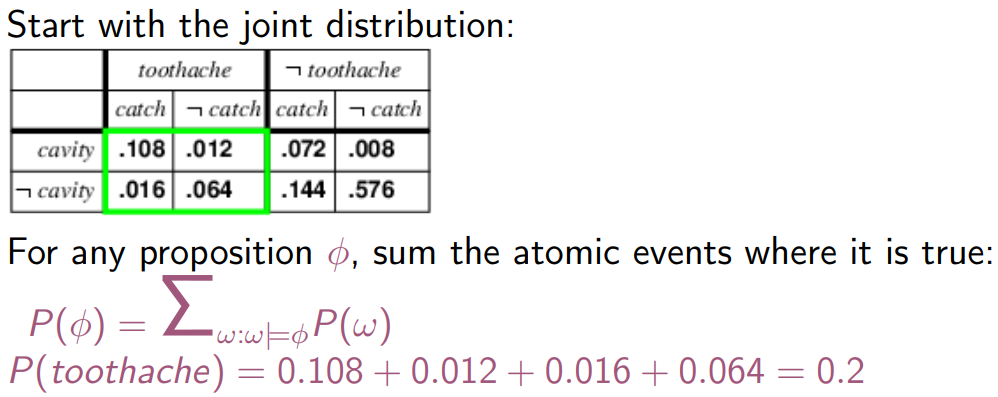
\includegraphics[width=0.7\textwidth]{inference.png}
\end{figure}

\section{Indipendenza}
Le proposizioni $a$ e $b$ sono \textit{indipendenti} se e solo se $P(a|b) = P(a)$ oppure $P(b|a) = P(b)$ oppure $P(a \wedge b) = P(a)P(b)$. L'\textit{indipendenza assoluta} tra sottoinsiemi di variabili casuali può consentire di fattorizzare la distribuzione congiunta completa in distribuzioni congiunte più piccole. Questo può ridurre drasticamente la complessità, ma raramente si verifica nella pratica.

\subsection{La regola di Bayes e il suo utilizzo}
La \textit{regola di Bayes} permette di calcolare probabilità sconosciute partendo da probabilità condizionate note, solitamente in direzione casuale. In presenza di molti elementi di prova, l'applicazione della regola di Bayes avrà in generale gli stessi problemi di scalabilità dell'uso diretto della distribuzione congiunta completa. L'\textit{equazione} della regola di Bayes è:
\[ P(a|b) = \frac{P(b|a)P(a)}{P(b)} \]

\subsection{Indipendenza condizionale}
L'\textit{indipendenza condizionale} dovuta a relazioni casuali dirette nel dominio può permettere di fattorizzare la distribuzione congiunta completa in distribuzioni condizionate più piccole. Il \textit{modello di Bayes ingenuo} assume come ipotesi l'indipendenza condizionale di tutte le variabili effetto data una singola variabile causa e cresce linearmente con il numero di effetti. In tal caso, quindi, la distribuzione congiunta completa può essere scritta come:
\[ P(Causa, Effetto_1, ..., Effetto_n) = P(Causa) \prod_i P(Effetto_i|Causa) \]

\section{Il mondo del wumpus}
Un agente del \textit{mondo del wumpus} può calcolare le probabilità degli aspetti del mondo non osservati e avvalersene per prendere decisioni migliori di quelle di un agente puramente logico.
\begin{figure}[htp]
	\begin{subfigure}{0.49\textwidth}
	    \centering
		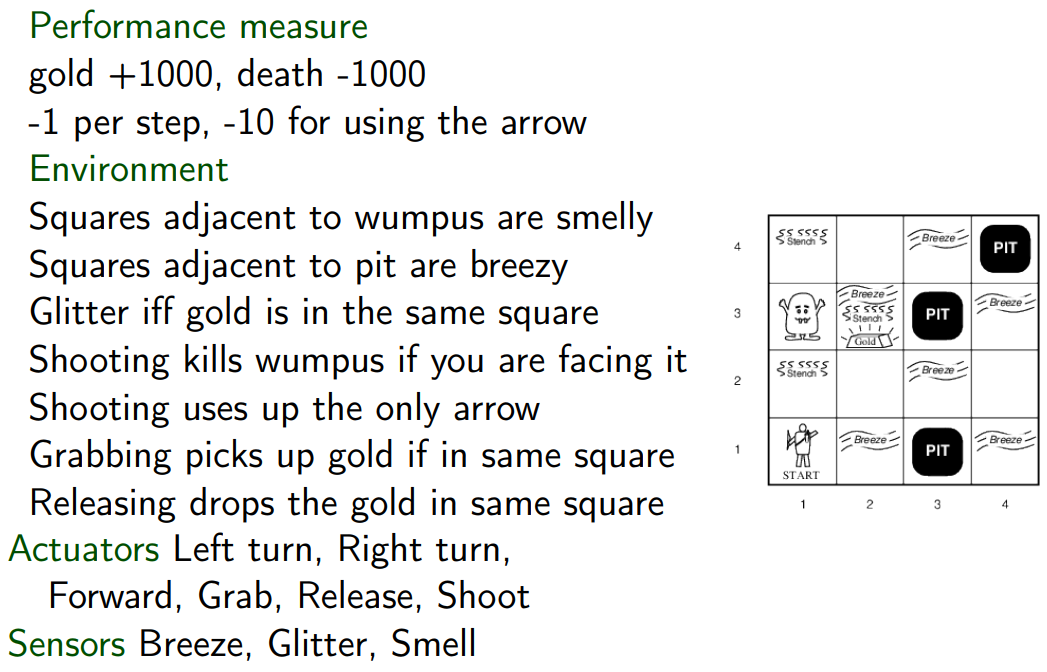
\includegraphics[width=0.9\textwidth]{wumpus-description.png}
		\caption{Descrizione del mondo del wumpus}
	\end{subfigure}
	\hfill
	\begin{subfigure}{0.49\textwidth}
	    \centering
		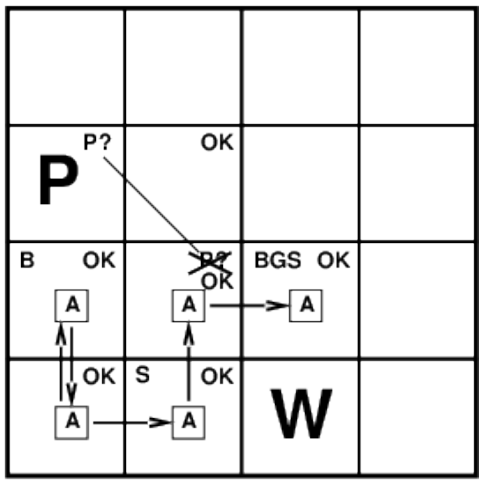
\includegraphics[width=0.55\textwidth]{wumpus-exploration0.png}
		\caption{Esempio di esplorazione}
	\end{subfigure}
\end{figure}

Nella \textit{figura (a)} sottostante si può notare che, dopo aver rilevato uno spostamento d'aria sia in $[1,2]$ che in $[2,1]$, l'agente si blocca in quanto non c'è più alcuna stanza sicura da esplorare. L'agente dovrà quindi fare un'interrogazione, ad esempio per $[1,3]$, suddividendo le stanze come mostrato nella \textit{figura (b)} sottostante.
\begin{figure}[htp]
	\begin{subfigure}{0.49\textwidth}
	    \centering
		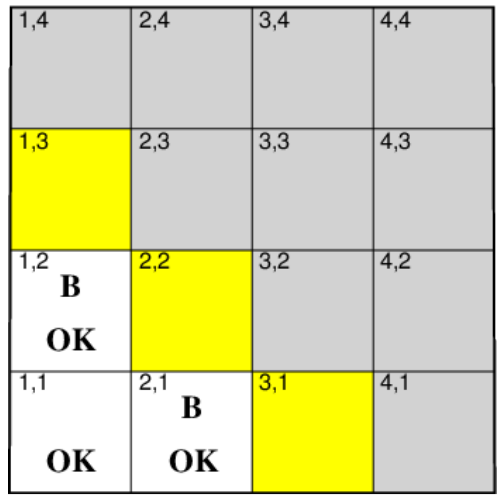
\includegraphics[width=0.55\textwidth]{wumpus-exploration1.png}
		\caption{}
	\end{subfigure}
	\hfill
	\begin{subfigure}{0.49\textwidth}
	    \centering
		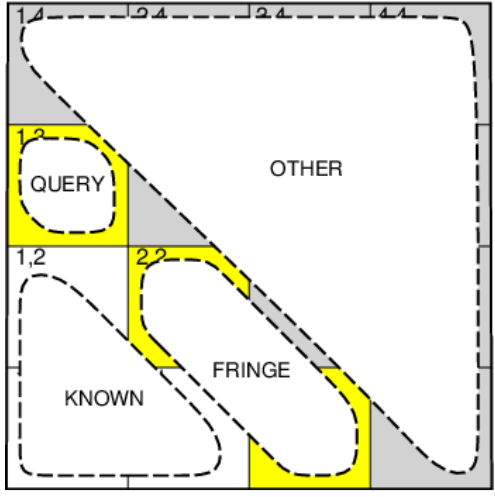
\includegraphics[width=0.55\textwidth]{wumpus-exploration2.png}
		\caption{}
	\end{subfigure}
\end{figure}

A seguito dell'interrogazione si otterranno i seguenti \textit{modelli} consistenti per le variabili di frontiera $P_{2,2}$ e $P_{3,1}$ (con l'indicazione di $P(frontiera)$ sotto ad ogni modello):
\begin{enumerate}[label=(\alph*)]
    \item Tre modelli con $P_{1,3} = true$ e la presenza di due o tre pozzi.
    \item Due modelli con $P_{1,3} = false$ e la presenza di uno o due pozzi.
\end{enumerate}
\begin{figure}[htp]
	\begin{subfigure}{0.49\textwidth}
	    \centering
		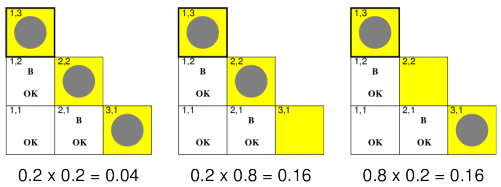
\includegraphics[width=\textwidth, height=\textheight, keepaspectratio]{modelli1.png}
		\caption{}
	\end{subfigure}
	\hfill
	\begin{subfigure}{0.49\textwidth}
	    \centering
		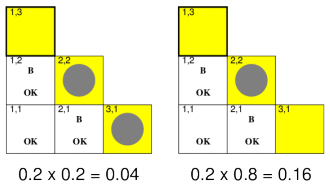
\includegraphics[width=0.65\textwidth]{modelli2.png}
		\caption{}
	\end{subfigure}
\end{figure}


\chapter{Problemi di decisione sequenziali}

\section{Decisioni complesse}
Quando dobbiamo prendere \textit{decisioni complesse}, occorre sfruttare la nostra conoscenza del mondo per prendere tali decisioni anche quando le loro conseguenze sono incerte, e le eventuali ricompense potrebbero non essere disponibili finché non sono state compiute diverse altre azioni.

\subsection{Markov Decision Processes}
I problemi di decisione sequenziali in ambienti incerti, chiamati anche \textit{processi decisionali di Markov} (MDP), sono definiti da:
\begin{itemize}
    \item Un \textit{modello di transizione}, che specifica gli esiti probabilistici delle azioni.
    \item Una \textit{funzione di ricompensa}, che specifica la ricompensa associata ad ogni stato.
\end{itemize}
\begin{figure}[htp]
	\centering
	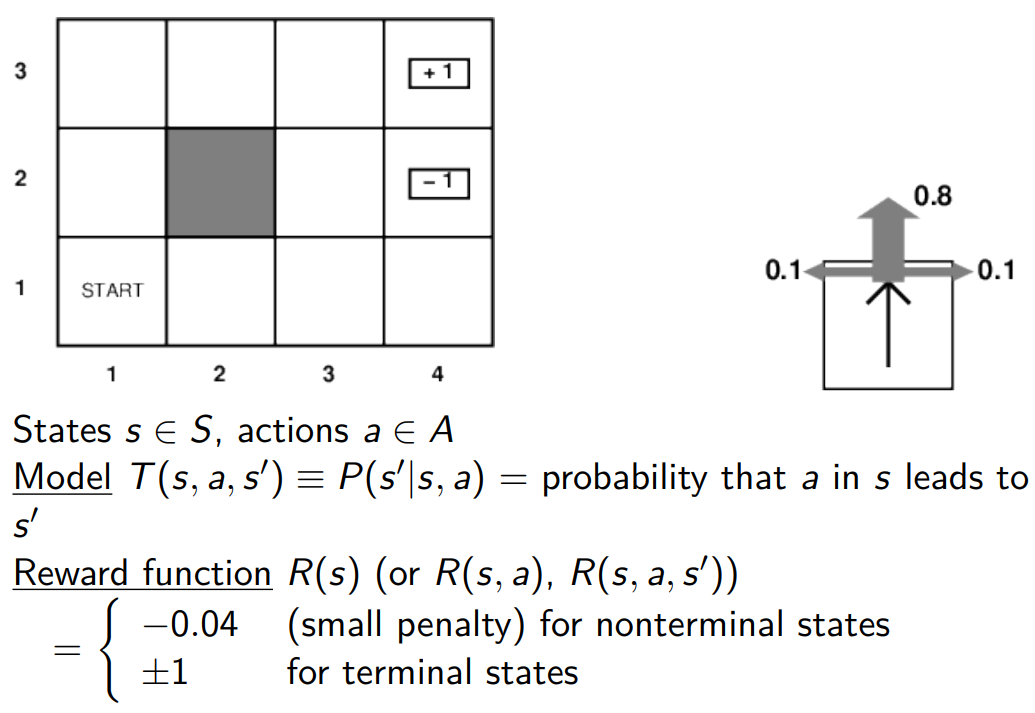
\includegraphics[width=0.8\textwidth]{mdp1.png}
\end{figure}

\subsection{La necessità delle politiche}
L'utilità di una sequenza di stati è pari alla somma di tutte le ricompense degli stati che contiene, con un possibile sconto dipendente dal tempo. La soluzione di un MDP sarà quindi una \textit{politica} (policy) che associa una decisione ad ogni stato raggiungibile dall'agente. Una politica ottima massimizza l'utilità delle sequenze di stati attraversati durante la sua esecuzione, ovvero trova la migliore azione per ogni possibile stato.
\begin{figure}[htp]
	\begin{subfigure}{0.49\textwidth}
	    \centering
		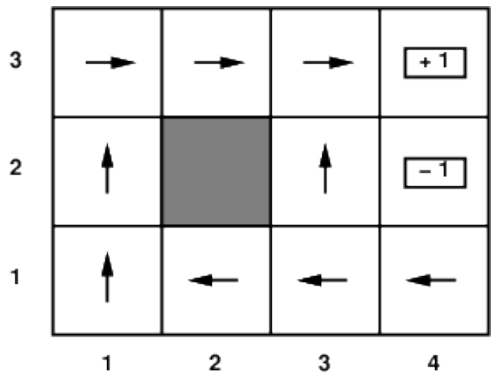
\includegraphics[width=\textwidth, height=\textheight, keepaspectratio]{policy1.png}
		\caption{Policy ottima con $R(s)=-0,04$}
	\end{subfigure}
	\hfill
	\begin{subfigure}{0.49\textwidth}
	    \centering
		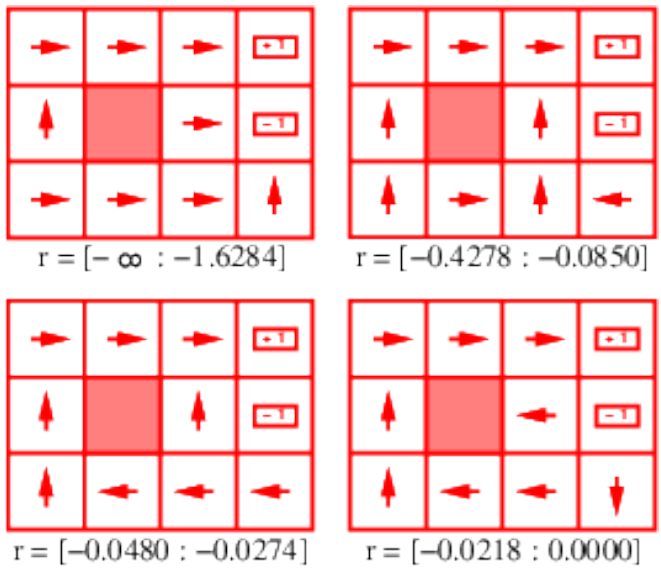
\includegraphics[width=0.9\textwidth]{policy2.png}
		\caption{Policy ottime per quattro diversi intervalli di $R(s)$}
	\end{subfigure}
\end{figure}

\section{Iterazione dei valori}
L'utilità di uno stato corrisponde all'utilità attesa delle sequenze di stati attraversati eseguendo una politica ottima partendo da esso. L'algoritmo di \textit{iterazione dei valori} per la soluzione degli MDP funziona risolvendo iterativamente le equazioni che collegano l'utilità di ogni stato a quella dei suoi vicini.
\begin{figure}[htp]
	\begin{subfigure}{0.49\textwidth}
	    \centering
		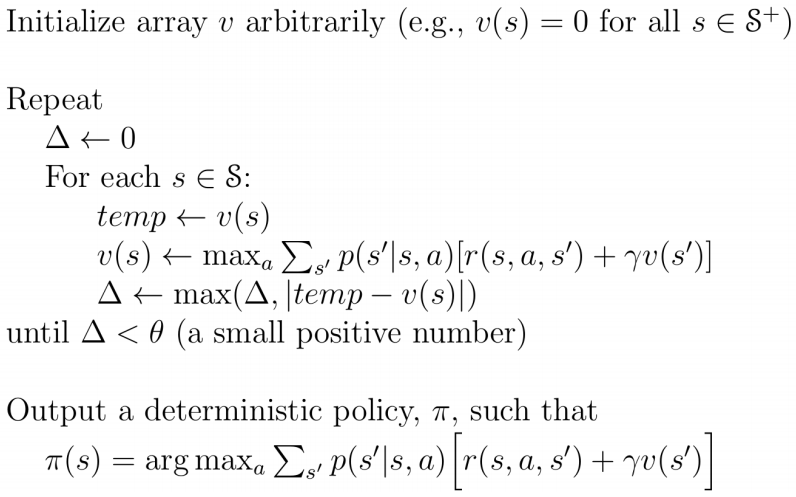
\includegraphics[width=\textwidth, height=\textheight, keepaspectratio]{value-iteration1.png}
		\caption{Algoritmo di iterazione dei valori}
	\end{subfigure}
	\hfill
	\begin{subfigure}{0.49\textwidth}
	    \centering
		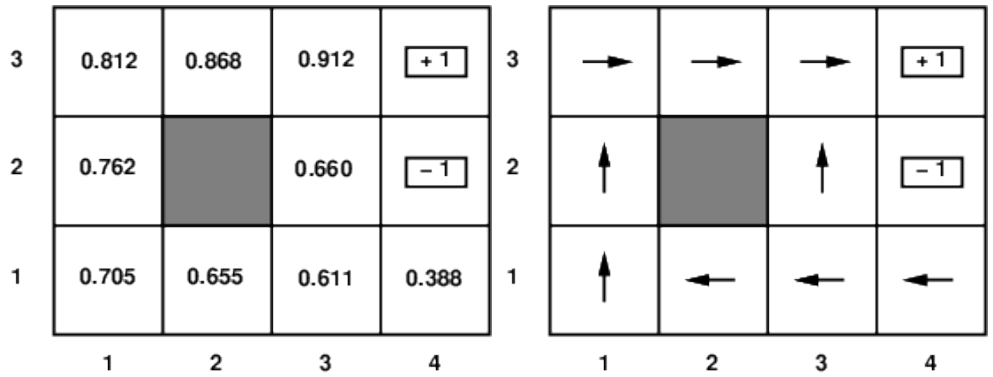
\includegraphics[width=\textwidth, height=\textheight, keepaspectratio]{value-iteration2.png}
		\caption{Utilità degli stati e policy}
	\end{subfigure}
\end{figure}

\section{Iterazione delle politiche}
L'\textit{iterazione delle politiche} alterna il calcolo delle utilità degli stati rispetto alla politica corrente (policy evaluation) con il miglioramento della politica in base alle utilità correnti (policy improvement). L'\textit{algoritmo} ripete policy evaluation e policy improvement fino a quando non è più possibile migliorare, garantendo quindi l'ottimalità della politica.
\begin{figure}[htp]
	\centering
	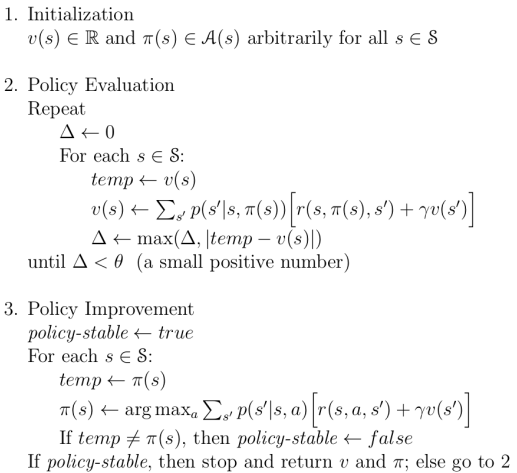
\includegraphics[width=0.6\textwidth]{policy-iteration.png}
\end{figure}

\section{MDP parzialmente osservabili}
Gli MDP parzialmente osservabili (\textit{POMDP}) sono molto più difficili da risolvere degli MDP. Infatti, la policy ottima in un POMDP è una funzione $\pi(b)$ dove $b$ è lo stato-credenza, in quanto l'agente non sa in quale stato si trova. \`{E} quindi possibile convertire un POMDP in un MDP nello spazio continuo degli stati-credenza. Il comportamento ottimo in un POMDP include la \textit{raccolta di informazioni} per ridurre l'incertezza e prendere decisioni migliori.
\begin{figure}[htp]
	\centering
	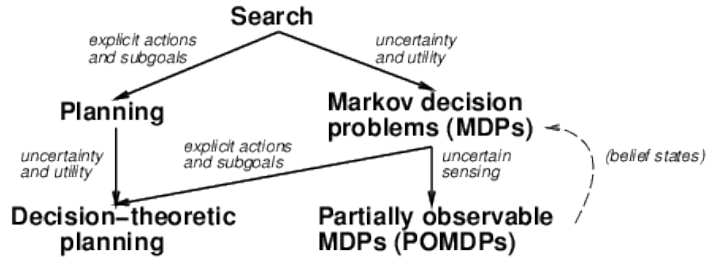
\includegraphics[width=0.8\textwidth]{mdp2.png}
\end{figure}


\chapter{Apprendimento per rinforzo}

\section{Introduzione}
Il problema dell'\textit{apprendimento per rinforzo} riguarda come un agente può imparare a comportarsi efficacemente in un ambiente sconosciuto, date solo le sue percezioni e occasionali ricompense. L'apprendimento per rinforzo può essere considerato un microcosmo per l'intero problema dell'IA, ma per facilitare i progressi viene studiato in diverse configurazioni semplificate.

\subsection{Progetto globale}
Il \textit{progetto globale} dell'agente determina il tipo di informazione che deve essere appresa. I progetti principali sono quelli:
\begin{itemize}
    \item \textit{Basati su modello} (model-based), che utilizzano un modello e una funzione di utilità.
    \item \textit{Privi di modello} (model-free), che utilizzano una funzione azione-valore.
\end{itemize}
\begin{figure}[htp]
	\begin{subfigure}{0.49\textwidth}
	    \centering
		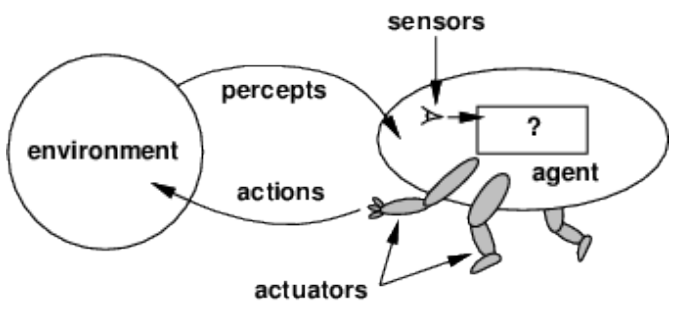
\includegraphics[width=\textwidth, height=\textheight, keepaspectratio]{rl1.png}
		\caption{Reinforcement learning (idea di base)}
	\end{subfigure}
	\hfill
	\begin{subfigure}{0.49\textwidth}
	    \centering
		\includegraphics[width=\textwidth, height=\textheight, keepaspectratio]{rl2.png}
		\caption{Model-based vs model-free}
	\end{subfigure}
\end{figure}

\section{Metodi model-based}
I metodi \textit{model-based} apprendono un modello e una funzione ricompensa dalle osservazioni e quindi utilizzano l'iterazione dei valori o delle politiche per ottenere le utilità o una politica ottima.
\begin{figure}[htp]
	\centering
	\includegraphics[width=\textwidth, height=\textheight, keepaspectratio]{rl3.png}
\end{figure}

\section{Metodi model-free}
I metodi \textit{model-free} aggiornano le stime di utilità in modo che si accordino con quelle degli stati successori. Usare un modello appreso per generare pseudo-esperienze, comunque, può velocizzare l'apprendimento.

\subsection{Q-Learning}
Il \textit{Q-Learning} non richiede alcun modello, né per l'apprendimento né in fase di selezione delle azioni. Questo semplifica il problema ma potenzialmente riduce la capacità di apprendere in ambienti complessi, perché l'agente non può simulare i risultati di possibili corsi d'azione.

\subsection{Sfruttamento ed esplorazione}
Q-Learning è un algoritmo \textit{off-policy}, ovvero impara la policy ottima senza seguirla ma arriva a risultati sub-ottimi, in quanto il modello appreso non coincide con l'ambiente vero (ciò che è ottimo nel modello potrebbe non esserlo nell'ambiente). Infatti, siccome l'agente non conosce l'ambiente reale, non può riuscire a calcolare l'azione realmente ottima. Quello che l'agente non considera è che le azioni non si limitano a fornire ricompense in base al modello appreso corrente, ma contribuiscono anche ad apprendere il modello vero influenzando le percezioni ricevute. Un agente deve quindi gestire il compromesso tra lo \textit{sfruttamento} (exploitation), che massimizza la ricompensa calcolata in base alle stime correnti di utilità, e l'\textit{esplorazione} (exploration), che massimizza il benessere a lungo termine. In generale, non è possibile trovare una soluzione esatta al problema dell'esplorazione, ma esistono semplici euristiche che permettono di ottenere risultati accettabili (ad esempio \textit{$\epsilon$-greedy} e \textit{soft-max}).
\begin{figure}[htp]
	\begin{subfigure}{0.49\textwidth}
	    \centering
		\includegraphics[width=\textwidth, height=\textheight, keepaspectratio]{q-learning1.png}
		\caption{Algoritmo Q-Learning}
	\end{subfigure}
	\hfill
	\begin{subfigure}{0.49\textwidth}
	    \centering
		\includegraphics[width=\textwidth, height=\textheight, keepaspectratio]{q-learning2.png}
		\caption{Exploration vs exploitation}
	\end{subfigure}
\end{figure}

\subsection{SARSA}
\textit{SARSA} è un algoritmo model-free alternativo a Q-Learning caratterizzato dal fatto che calcola la prossima azione basandosi sulla policy (algoritmo \textit{on-policy}). Confrontiamo brevemente i due algoritmi:
\begin{itemize}
    \item \textit{Q-Learning} impara la policy ottima ma a volte fallisce a causa della selezione dell'azione con $\epsilon$-greedy.
    \item \textit{SARSA}, essendo on-policy, ha migliori performance on-line.
\end{itemize}
\begin{figure}[htp]
	\begin{subfigure}{0.49\textwidth}
	    \centering
		\includegraphics[width=\textwidth, height=\textheight, keepaspectratio]{sarsa1.png}
		\caption{Algoritmo SARSA}
	\end{subfigure}
	\hfill
	\begin{subfigure}{0.49\textwidth}
	    \centering
		\includegraphics[width=\textwidth, height=\textheight, keepaspectratio]{sarsa2.png}
		\caption{Q-Learning vs SARSA}
	\end{subfigure}
\end{figure}


\section{Deep reinforcement learning}
Il \textit{deep reinforcement learning} è una delle aree di ricerca più attive nel campo dell'IA. In particolare, le applicazioni alla robotica sono quelle che promettono meglio; in questo campo infatti si devono gestire ambienti continui, a molte dimensioni e parzialmente osservabili in cui i comportamenti di successo possono essere composti anche da migliaia di azioni primitive. Quindi, nel momento in cui gli spazi degli stati diventano molto grandi, gli algoritmi di apprendimento per rinforzo devono ricorrere ad una rappresentazione approssimata della funzione $Q(s,a)$ (\textit{Q-Function}) per poter generalizzare. Una rappresentazione possibile sono le \textit{reti neurali}.

\subsection{Deep Neural Networks}
Le \textit{DNN} (Deep Neural Networks) possono approssimare arbitrariamente bene un ampio insieme di stati. Le DNN usano \textit{gradient descent} e \textit{back propagation} per imparare il modello.
\begin{figure}[htp]
	\begin{subfigure}{0.49\textwidth}
	    \centering
		\includegraphics[width=\textwidth, height=\textheight, keepaspectratio]{dnn1.png}
		\caption{Rete neurale}
	\end{subfigure}
	\hfill
	\begin{subfigure}{0.49\textwidth}
	    \centering
		\includegraphics[width=\textwidth, height=\textheight, keepaspectratio]{dnn2.png}
		\caption{Gradient descent e back propagation}
	\end{subfigure}
\end{figure}

\subsection{Deep Q-Network}
\textit{Deep Q-Network} è un potente approccio usato per eseguire deep reinforcement learning in spazi di azione discreti. Deep Q-Network approssima $Q(s,a)$ con una DNN; in particolare, usa \textit{experience replay} (mini-batch) e due reti differenti (Q-network e target network) per mitigare la divergenza dell'algoritmo \textit{Gradient Q-Learning} su cui esso si basa.
\begin{figure}[htp]
	\begin{subfigure}{0.49\textwidth}
	    \centering
		\includegraphics[width=\textwidth, height=\textheight, keepaspectratio]{dqn1.png}
		\caption{Gradient Q-Learning}
	\end{subfigure}
	\hfill
	\begin{subfigure}{0.49\textwidth}
	    \centering
		\includegraphics[width=\textwidth, height=\textheight, keepaspectratio]{dqn2.png}
		\caption{Deep Q-Network}
	\end{subfigure}
\end{figure}


% INIZIO CODICE LABORATORIO ==================================================================
\appendix
\chapter{Codici dei programmi del laboratorio}

% Sessione 1 - Ricerca non informata
\phantomsection
\begin{tcolorbox}[breakable, size=fbox, boxrule=1pt, pad at break*=1mm,colback=cellbackground, colframe=cellborder, title=Sessione 1 - Ricerca non informata, addtolol]
\prompt{In}{incolor}{1}{\boxspacing}
\begin{Verbatim}[commandchars=\\\{\}]
\PY{k+kn}{import} \PY{n+nn}{os}\PY{o}{,} \PY{n+nn}{sys}\PY{o}{,} \PY{n+nn}{time}\PY{o}{,} \PY{n+nn}{math}

\PY{n}{module\PYZus{}path} \PY{o}{=} \PY{n}{os}\PY{o}{.}\PY{n}{path}\PY{o}{.}\PY{n}{abspath}\PY{p}{(}\PY{n}{os}\PY{o}{.}\PY{n}{path}\PY{o}{.}\PY{n}{join}\PY{p}{(}\PY{l+s+s1}{\PYZsq{}}\PY{l+s+s1}{../tools}\PY{l+s+s1}{\PYZsq{}}\PY{p}{)}\PY{p}{)}
\PY{k}{if} \PY{n}{module\PYZus{}path} \PY{o+ow}{not} \PY{o+ow}{in} \PY{n}{sys}\PY{o}{.}\PY{n}{path}\PY{p}{:}
    \PY{n}{sys}\PY{o}{.}\PY{n}{path}\PY{o}{.}\PY{n}{append}\PY{p}{(}\PY{n}{module\PYZus{}path}\PY{p}{)}

\PY{k+kn}{from} \PY{n+nn}{utils}\PY{n+nn}{.}\PY{n+nn}{ai\PYZus{}lab\PYZus{}functions} \PY{k+kn}{import} \PY{o}{*}
\PY{k+kn}{import} \PY{n+nn}{gym}\PY{o}{,} \PY{n+nn}{envs}


\PY{c+c1}{\PYZsh{} ***Assignment 1: Breadth\PYZhy{}First Search (BFS)***}

\PY{k}{def} \PY{n+nf}{BFS\PYZus{}TreeSearch}\PY{p}{(}\PY{n}{problem}\PY{p}{)}\PY{p}{:}
    \PY{l+s+sd}{\PYZdq{}\PYZdq{}\PYZdq{}}
\PY{l+s+sd}{    Tree Search BFS}
\PY{l+s+sd}{    }
\PY{l+s+sd}{    Args:}
\PY{l+s+sd}{        problem: OpenAI Gym environment}
\PY{l+s+sd}{        }
\PY{l+s+sd}{    Returns:}
\PY{l+s+sd}{        (path, time\PYZus{}cost, space\PYZus{}cost): solution as a path and stats.}
\PY{l+s+sd}{    \PYZdq{}\PYZdq{}\PYZdq{}}
    
    \PY{n}{node} \PY{o}{=} \PY{n}{Node}\PY{p}{(}\PY{n}{problem}\PY{o}{.}\PY{n}{startstate}\PY{p}{,} \PY{k+kc}{None}\PY{p}{)}
    \PY{n}{time\PYZus{}cost} \PY{o}{=} \PY{l+m+mi}{0}
    \PY{n}{space\PYZus{}cost} \PY{o}{=} \PY{l+m+mi}{0}
    
    \PY{k}{if} \PY{n}{node}\PY{o}{.}\PY{n}{state} \PY{o}{==} \PY{n}{problem}\PY{o}{.}\PY{n}{goalstate}\PY{p}{:}
        \PY{k}{return} \PY{n}{build\PYZus{}path}\PY{p}{(}\PY{n}{node}\PY{p}{)}\PY{p}{,} \PY{n}{time\PYZus{}cost}\PY{p}{,} \PY{n}{space\PYZus{}cost}
    \PY{n}{frontier} \PY{o}{=} \PY{n}{NodeQueue}\PY{p}{(}\PY{p}{)}
    \PY{n}{frontier}\PY{o}{.}\PY{n}{add}\PY{p}{(}\PY{n}{node}\PY{p}{)}
    \PY{n}{space\PYZus{}cost} \PY{o}{+}\PY{o}{=} \PY{l+m+mi}{1}
    
    \PY{k}{while} \PY{k+kc}{True}\PY{p}{:}
        \PY{k}{if} \PY{n}{frontier}\PY{o}{.}\PY{n}{is\PYZus{}empty}\PY{p}{(}\PY{p}{)}\PY{p}{:}
            \PY{k}{return} \PY{l+s+s2}{\PYZdq{}}\PY{l+s+s2}{failure}\PY{l+s+s2}{\PYZdq{}}\PY{p}{,} \PY{n}{time\PYZus{}cost}\PY{p}{,} \PY{n}{space\PYZus{}cost}
        \PY{n}{node} \PY{o}{=} \PY{n}{frontier}\PY{o}{.}\PY{n}{remove}\PY{p}{(}\PY{p}{)}
        
        \PY{n}{space\PYZus{}cost} \PY{o}{\PYZhy{}}\PY{o}{=} \PY{l+m+mi}{1} \PY{c+c1}{\PYZsh{}space\PYZus{}cost è la dimensione massima di frontier}
        \PY{k}{for} \PY{n}{action} \PY{o+ow}{in} \PY{n+nb}{range}\PY{p}{(}\PY{n}{problem}\PY{o}{.}\PY{n}{action\PYZus{}space}\PY{o}{.}\PY{n}{n}\PY{p}{)}\PY{p}{:}
            \PY{n}{child} \PY{o}{=} \PY{n}{Node}\PY{p}{(}\PY{n}{problem}\PY{o}{.}\PY{n}{sample}\PY{p}{(}\PY{n}{node}\PY{o}{.}\PY{n}{state}\PY{p}{,} \PY{n}{action}\PY{p}{)}\PY{p}{,} \PY{n}{node}\PY{p}{)}
            \PY{c+c1}{\PYZsh{}if child.state not in explored and child.state not in frontier: \PYZsh{}posso visitare più volte lo stesso stato!}
            \PY{k}{if} \PY{n}{child}\PY{o}{.}\PY{n}{state} \PY{o}{==} \PY{n}{problem}\PY{o}{.}\PY{n}{goalstate}\PY{p}{:}
                \PY{k}{return} \PY{n}{build\PYZus{}path}\PY{p}{(}\PY{n}{child}\PY{p}{)}\PY{p}{,} \PY{n}{time\PYZus{}cost}\PY{p}{,} \PY{n}{space\PYZus{}cost}
            \PY{n}{frontier}\PY{o}{.}\PY{n}{add}\PY{p}{(}\PY{n}{child}\PY{p}{)}
            \PY{n}{space\PYZus{}cost} \PY{o}{+}\PY{o}{=} \PY{l+m+mi}{1}
            \PY{n}{time\PYZus{}cost} \PY{o}{+}\PY{o}{=} \PY{l+m+mi}{1} \PY{c+c1}{\PYZsh{}time\PYZus{}cost++ ogni volta che creo un figlio}

\PY{k}{def} \PY{n+nf}{BFS\PYZus{}GraphSearch}\PY{p}{(}\PY{n}{problem}\PY{p}{)}\PY{p}{:}
    \PY{l+s+sd}{\PYZdq{}\PYZdq{}\PYZdq{}}
\PY{l+s+sd}{    Graph Search BFS}
\PY{l+s+sd}{    }
\PY{l+s+sd}{    Args:}
\PY{l+s+sd}{        problem: OpenAI Gym environment}
\PY{l+s+sd}{        }
\PY{l+s+sd}{    Returns:}
\PY{l+s+sd}{        (path, time\PYZus{}cost, space\PYZus{}cost): solution as a path and stats.}
\PY{l+s+sd}{    \PYZdq{}\PYZdq{}\PYZdq{}}
    
    \PY{n}{node} \PY{o}{=} \PY{n}{Node}\PY{p}{(}\PY{n}{problem}\PY{o}{.}\PY{n}{startstate}\PY{p}{,} \PY{k+kc}{None}\PY{p}{)}
    
    \PY{n}{time\PYZus{}cost} \PY{o}{=} \PY{l+m+mi}{0}
    \PY{n}{space\PYZus{}cost} \PY{o}{=} \PY{l+m+mi}{0}
    
    \PY{k}{if} \PY{n}{node}\PY{o}{.}\PY{n}{state} \PY{o}{==} \PY{n}{problem}\PY{o}{.}\PY{n}{goalstate}\PY{p}{:}
        \PY{k}{return} \PY{n}{build\PYZus{}path}\PY{p}{(}\PY{n}{node}\PY{p}{)}\PY{p}{,} \PY{n}{time\PYZus{}cost}\PY{p}{,} \PY{n}{space\PYZus{}cost}
    \PY{n}{frontier} \PY{o}{=} \PY{n}{NodeQueue}\PY{p}{(}\PY{p}{)}
    \PY{n}{frontier}\PY{o}{.}\PY{n}{add}\PY{p}{(}\PY{n}{node}\PY{p}{)}
    \PY{n}{explored} \PY{o}{=} \PY{n+nb}{set}\PY{p}{(}\PY{p}{)}
    \PY{k}{while} \PY{k+kc}{True}\PY{p}{:}
        \PY{k}{if} \PY{n}{frontier}\PY{o}{.}\PY{n}{is\PYZus{}empty}\PY{p}{(}\PY{p}{)}\PY{p}{:}
            \PY{k}{return} \PY{l+s+s2}{\PYZdq{}}\PY{l+s+s2}{failure}\PY{l+s+s2}{\PYZdq{}}\PY{p}{,} \PY{n}{time\PYZus{}cost}\PY{p}{,} \PY{n}{space\PYZus{}cost}
        \PY{n}{node} \PY{o}{=} \PY{n}{frontier}\PY{o}{.}\PY{n}{remove}\PY{p}{(}\PY{p}{)}
        \PY{n}{explored}\PY{o}{.}\PY{n}{add}\PY{p}{(}\PY{n}{node}\PY{o}{.}\PY{n}{state}\PY{p}{)}
        \PY{n}{space\PYZus{}cost} \PY{o}{+}\PY{o}{=} \PY{l+m+mi}{1} \PY{c+c1}{\PYZsh{}space\PYZus{}cost è la dimensione massima di explored}
        \PY{k}{for} \PY{n}{action} \PY{o+ow}{in} \PY{n+nb}{range}\PY{p}{(}\PY{n}{problem}\PY{o}{.}\PY{n}{action\PYZus{}space}\PY{o}{.}\PY{n}{n}\PY{p}{)}\PY{p}{:}
            \PY{n}{child} \PY{o}{=} \PY{n}{Node}\PY{p}{(}\PY{n}{problem}\PY{o}{.}\PY{n}{sample}\PY{p}{(}\PY{n}{node}\PY{o}{.}\PY{n}{state}\PY{p}{,} \PY{n}{action}\PY{p}{)}\PY{p}{,} \PY{n}{node}\PY{p}{)}
            \PY{k}{if} \PY{n}{child}\PY{o}{.}\PY{n}{state} \PY{o+ow}{not} \PY{o+ow}{in} \PY{n}{explored} \PY{o+ow}{and} \PY{n}{child}\PY{o}{.}\PY{n}{state} \PY{o+ow}{not} \PY{o+ow}{in} \PY{n}{frontier}\PY{p}{:}
                \PY{k}{if} \PY{n}{child}\PY{o}{.}\PY{n}{state} \PY{o}{==} \PY{n}{problem}\PY{o}{.}\PY{n}{goalstate}\PY{p}{:}
                    \PY{k}{return} \PY{n}{build\PYZus{}path}\PY{p}{(}\PY{n}{child}\PY{p}{)}\PY{p}{,} \PY{n}{time\PYZus{}cost}\PY{p}{,} \PY{n}{space\PYZus{}cost}
                \PY{n}{frontier}\PY{o}{.}\PY{n}{add}\PY{p}{(}\PY{n}{child}\PY{p}{)}
            \PY{n}{time\PYZus{}cost} \PY{o}{+}\PY{o}{=} \PY{l+m+mi}{1} \PY{c+c1}{\PYZsh{}time\PYZus{}cost++ ogni volta che creo un figlio}


\PY{c+c1}{\PYZsh{} The following code calls your tree search and graph search version of BFS and prints the results:}

\PY{n}{envname} \PY{o}{=} \PY{l+s+s2}{\PYZdq{}}\PY{l+s+s2}{SmallMaze\PYZhy{}v0}\PY{l+s+s2}{\PYZdq{}}
\PY{n}{environment} \PY{o}{=} \PY{n}{gym}\PY{o}{.}\PY{n}{make}\PY{p}{(}\PY{n}{envname}\PY{p}{)}

\PY{n}{solution\PYZus{}ts}\PY{p}{,} \PY{n}{time\PYZus{}ts}\PY{p}{,} \PY{n}{memory\PYZus{}ts} \PY{o}{=} \PY{n}{BFS\PYZus{}TreeSearch}\PY{p}{(}\PY{n}{environment}\PY{p}{)}
\PY{n}{solution\PYZus{}gs}\PY{p}{,} \PY{n}{time\PYZus{}gs}\PY{p}{,} \PY{n}{memory\PYZus{}gs} \PY{o}{=} \PY{n}{BFS\PYZus{}GraphSearch}\PY{p}{(}\PY{n}{environment}\PY{p}{)}

\PY{n+nb}{print}\PY{p}{(}\PY{l+s+s2}{\PYZdq{}}\PY{l+s+se}{\PYZbs{}n}\PY{l+s+s2}{\PYZhy{}\PYZhy{}\PYZhy{}\PYZhy{}\PYZhy{}\PYZhy{}\PYZhy{}\PYZhy{}\PYZhy{}\PYZhy{}\PYZhy{}\PYZhy{}\PYZhy{}\PYZhy{}\PYZhy{}\PYZhy{}\PYZhy{}\PYZhy{}\PYZhy{}\PYZhy{}\PYZhy{}\PYZhy{}\PYZhy{}\PYZhy{}\PYZhy{}\PYZhy{}\PYZhy{}\PYZhy{}\PYZhy{}\PYZhy{}\PYZhy{}\PYZhy{}\PYZhy{}\PYZhy{}\PYZhy{}\PYZhy{}\PYZhy{}\PYZhy{}\PYZhy{}\PYZhy{}\PYZhy{}\PYZhy{}\PYZhy{}\PYZhy{}\PYZhy{}\PYZhy{}\PYZhy{}\PYZhy{}\PYZhy{}\PYZhy{}\PYZhy{}\PYZhy{}\PYZhy{}\PYZhy{}\PYZhy{}\PYZhy{}\PYZhy{}\PYZhy{}\PYZhy{}\PYZhy{}\PYZhy{}\PYZhy{}\PYZhy{}\PYZhy{}}\PY{l+s+s2}{\PYZdq{}}\PY{p}{)}
\PY{n+nb}{print}\PY{p}{(}\PY{l+s+s2}{\PYZdq{}}\PY{l+s+se}{\PYZbs{}t}\PY{l+s+s2}{BFS TREE SEARCH PROBLEM: }\PY{l+s+s2}{\PYZdq{}}\PY{p}{)}
\PY{n+nb}{print}\PY{p}{(}\PY{l+s+s2}{\PYZdq{}}\PY{l+s+s2}{\PYZhy{}\PYZhy{}\PYZhy{}\PYZhy{}\PYZhy{}\PYZhy{}\PYZhy{}\PYZhy{}\PYZhy{}\PYZhy{}\PYZhy{}\PYZhy{}\PYZhy{}\PYZhy{}\PYZhy{}\PYZhy{}\PYZhy{}\PYZhy{}\PYZhy{}\PYZhy{}\PYZhy{}\PYZhy{}\PYZhy{}\PYZhy{}\PYZhy{}\PYZhy{}\PYZhy{}\PYZhy{}\PYZhy{}\PYZhy{}\PYZhy{}\PYZhy{}\PYZhy{}\PYZhy{}\PYZhy{}\PYZhy{}\PYZhy{}\PYZhy{}\PYZhy{}\PYZhy{}\PYZhy{}\PYZhy{}\PYZhy{}\PYZhy{}\PYZhy{}\PYZhy{}\PYZhy{}\PYZhy{}\PYZhy{}\PYZhy{}\PYZhy{}\PYZhy{}\PYZhy{}\PYZhy{}\PYZhy{}\PYZhy{}\PYZhy{}\PYZhy{}\PYZhy{}\PYZhy{}\PYZhy{}\PYZhy{}\PYZhy{}\PYZhy{}}\PY{l+s+s2}{\PYZdq{}}\PY{p}{)}
\PY{n+nb}{print}\PY{p}{(}\PY{l+s+s2}{\PYZdq{}}\PY{l+s+s2}{Solution: }\PY{l+s+si}{\PYZob{}\PYZcb{}}\PY{l+s+s2}{\PYZdq{}}\PY{o}{.}\PY{n}{format}\PY{p}{(}\PY{n}{solution\PYZus{}2\PYZus{}string}\PY{p}{(}\PY{n}{solution\PYZus{}ts}\PY{p}{,} \PY{n}{environment}\PY{p}{)}\PY{p}{)}\PY{p}{)}
\PY{n+nb}{print}\PY{p}{(}\PY{l+s+s2}{\PYZdq{}}\PY{l+s+s2}{N° of nodes explored: }\PY{l+s+si}{\PYZob{}\PYZcb{}}\PY{l+s+s2}{\PYZdq{}}\PY{o}{.}\PY{n}{format}\PY{p}{(}\PY{n}{time\PYZus{}ts}\PY{p}{)}\PY{p}{)}
\PY{n+nb}{print}\PY{p}{(}\PY{l+s+s2}{\PYZdq{}}\PY{l+s+s2}{Max n° of nodes in memory: }\PY{l+s+si}{\PYZob{}\PYZcb{}}\PY{l+s+s2}{\PYZdq{}}\PY{o}{.}\PY{n}{format}\PY{p}{(}\PY{n}{memory\PYZus{}ts}\PY{p}{)}\PY{p}{)}

\PY{n+nb}{print}\PY{p}{(}\PY{l+s+s2}{\PYZdq{}}\PY{l+s+se}{\PYZbs{}n}\PY{l+s+s2}{\PYZhy{}\PYZhy{}\PYZhy{}\PYZhy{}\PYZhy{}\PYZhy{}\PYZhy{}\PYZhy{}\PYZhy{}\PYZhy{}\PYZhy{}\PYZhy{}\PYZhy{}\PYZhy{}\PYZhy{}\PYZhy{}\PYZhy{}\PYZhy{}\PYZhy{}\PYZhy{}\PYZhy{}\PYZhy{}\PYZhy{}\PYZhy{}\PYZhy{}\PYZhy{}\PYZhy{}\PYZhy{}\PYZhy{}\PYZhy{}\PYZhy{}\PYZhy{}\PYZhy{}\PYZhy{}\PYZhy{}\PYZhy{}\PYZhy{}\PYZhy{}\PYZhy{}\PYZhy{}\PYZhy{}\PYZhy{}\PYZhy{}\PYZhy{}\PYZhy{}\PYZhy{}\PYZhy{}\PYZhy{}\PYZhy{}\PYZhy{}\PYZhy{}\PYZhy{}\PYZhy{}\PYZhy{}\PYZhy{}\PYZhy{}\PYZhy{}\PYZhy{}\PYZhy{}\PYZhy{}\PYZhy{}\PYZhy{}\PYZhy{}\PYZhy{}}\PY{l+s+s2}{\PYZdq{}}\PY{p}{)}
\PY{n+nb}{print}\PY{p}{(}\PY{l+s+s2}{\PYZdq{}}\PY{l+s+se}{\PYZbs{}t}\PY{l+s+s2}{BFS GRAPH SEARCH PROBLEM: }\PY{l+s+s2}{\PYZdq{}}\PY{p}{)}
\PY{n+nb}{print}\PY{p}{(}\PY{l+s+s2}{\PYZdq{}}\PY{l+s+s2}{\PYZhy{}\PYZhy{}\PYZhy{}\PYZhy{}\PYZhy{}\PYZhy{}\PYZhy{}\PYZhy{}\PYZhy{}\PYZhy{}\PYZhy{}\PYZhy{}\PYZhy{}\PYZhy{}\PYZhy{}\PYZhy{}\PYZhy{}\PYZhy{}\PYZhy{}\PYZhy{}\PYZhy{}\PYZhy{}\PYZhy{}\PYZhy{}\PYZhy{}\PYZhy{}\PYZhy{}\PYZhy{}\PYZhy{}\PYZhy{}\PYZhy{}\PYZhy{}\PYZhy{}\PYZhy{}\PYZhy{}\PYZhy{}\PYZhy{}\PYZhy{}\PYZhy{}\PYZhy{}\PYZhy{}\PYZhy{}\PYZhy{}\PYZhy{}\PYZhy{}\PYZhy{}\PYZhy{}\PYZhy{}\PYZhy{}\PYZhy{}\PYZhy{}\PYZhy{}\PYZhy{}\PYZhy{}\PYZhy{}\PYZhy{}\PYZhy{}\PYZhy{}\PYZhy{}\PYZhy{}\PYZhy{}\PYZhy{}\PYZhy{}\PYZhy{}}\PY{l+s+s2}{\PYZdq{}}\PY{p}{)}
\PY{n+nb}{print}\PY{p}{(}\PY{l+s+s2}{\PYZdq{}}\PY{l+s+s2}{Solution: }\PY{l+s+si}{\PYZob{}\PYZcb{}}\PY{l+s+s2}{\PYZdq{}}\PY{o}{.}\PY{n}{format}\PY{p}{(}\PY{n}{solution\PYZus{}2\PYZus{}string}\PY{p}{(}\PY{n}{solution\PYZus{}gs}\PY{p}{,} \PY{n}{environment}\PY{p}{)}\PY{p}{)}\PY{p}{)}
\PY{n+nb}{print}\PY{p}{(}\PY{l+s+s2}{\PYZdq{}}\PY{l+s+s2}{N° of nodes explored: }\PY{l+s+si}{\PYZob{}\PYZcb{}}\PY{l+s+s2}{\PYZdq{}}\PY{o}{.}\PY{n}{format}\PY{p}{(}\PY{n}{time\PYZus{}gs}\PY{p}{)}\PY{p}{)}
\PY{n+nb}{print}\PY{p}{(}\PY{l+s+s2}{\PYZdq{}}\PY{l+s+s2}{Max n° of nodes in memory: }\PY{l+s+si}{\PYZob{}\PYZcb{}}\PY{l+s+s2}{\PYZdq{}}\PY{o}{.}\PY{n}{format}\PY{p}{(}\PY{n}{memory\PYZus{}gs}\PY{p}{)}\PY{p}{)}


\PY{c+c1}{\PYZsh{} ***Assignment 2: Depth\PYZhy{}Limited Search (DLS) and Iterative Deepening depth\PYZhy{}first Search (IDS)***}

\PY{k}{def} \PY{n+nf}{DLS}\PY{p}{(}\PY{n}{problem}\PY{p}{,} \PY{n}{limit}\PY{p}{,} \PY{n}{RDLS\PYZus{}Function}\PY{p}{)}\PY{p}{:}
    \PY{l+s+sd}{\PYZdq{}\PYZdq{}\PYZdq{}}
\PY{l+s+sd}{    DLS}
\PY{l+s+sd}{    }
\PY{l+s+sd}{    Args:}
\PY{l+s+sd}{        problem: OpenAI Gym environment}
\PY{l+s+sd}{        limit: depth limit for the exploration, negative number means \PYZsq{}no limit\PYZsq{}}
\PY{l+s+sd}{        }
\PY{l+s+sd}{    Returns:}
\PY{l+s+sd}{        (path, time\PYZus{}cost, space\PYZus{}cost): solution as a path and stats.}
\PY{l+s+sd}{    \PYZdq{}\PYZdq{}\PYZdq{}}
    
    \PY{n}{node} \PY{o}{=} \PY{n}{Node}\PY{p}{(}\PY{n}{problem}\PY{o}{.}\PY{n}{startstate}\PY{p}{,} \PY{k+kc}{None}\PY{p}{)}
    \PY{k}{return} \PY{n}{RDLS\PYZus{}Function}\PY{p}{(}\PY{n}{node}\PY{p}{,} \PY{n}{problem}\PY{p}{,} \PY{n}{limit}\PY{p}{,} \PY{n+nb}{set}\PY{p}{(}\PY{p}{)}\PY{p}{)}

\PY{k}{def} \PY{n+nf}{Recursive\PYZus{}DLS\PYZus{}GraphSearch}\PY{p}{(}\PY{n}{node}\PY{p}{,} \PY{n}{problem}\PY{p}{,} \PY{n}{limit}\PY{p}{,} \PY{n}{closed}\PY{p}{)}\PY{p}{:}
    \PY{l+s+sd}{\PYZdq{}\PYZdq{}\PYZdq{}}
\PY{l+s+sd}{    Recursive DLS}
\PY{l+s+sd}{    }
\PY{l+s+sd}{    Args:}
\PY{l+s+sd}{        node: node to explore}
\PY{l+s+sd}{        problem: OpenAI Gym environment}
\PY{l+s+sd}{        limit: depth limit for the exploration, negative number means \PYZsq{}no limit\PYZsq{}}
\PY{l+s+sd}{        closed: completely explored nodes}
\PY{l+s+sd}{        }
\PY{l+s+sd}{    Returns:}
\PY{l+s+sd}{        (path, time\PYZus{}cost, space\PYZus{}cost): solution as a path and stats.}
\PY{l+s+sd}{    \PYZdq{}\PYZdq{}\PYZdq{}}
    
    \PY{n}{space\PYZus{}cost} \PY{o}{=} \PY{n}{node}\PY{o}{.}\PY{n}{pathcost}
    \PY{n}{time\PYZus{}cost} \PY{o}{=} \PY{l+m+mi}{1}
    
    \PY{k}{if} \PY{n}{node}\PY{o}{.}\PY{n}{state} \PY{o}{==} \PY{n}{problem}\PY{o}{.}\PY{n}{goalstate}\PY{p}{:}
        \PY{k}{return} \PY{n}{build\PYZus{}path}\PY{p}{(}\PY{n}{node}\PY{p}{)}\PY{p}{,} \PY{n}{time\PYZus{}cost}\PY{p}{,} \PY{n}{space\PYZus{}cost} \PY{c+c1}{\PYZsh{}ultimo passo: space\PYZus{}cost non cresce più e time\PYZus{}cost = 1}
    \PY{k}{elif} \PY{n}{limit} \PY{o}{==} \PY{l+m+mi}{0}\PY{p}{:}
        \PY{k}{return} \PY{l+s+s2}{\PYZdq{}}\PY{l+s+s2}{cut\PYZus{}off}\PY{l+s+s2}{\PYZdq{}}\PY{p}{,} \PY{n}{time\PYZus{}cost}\PY{p}{,} \PY{n}{space\PYZus{}cost}
    \PY{k}{else}\PY{p}{:}
        \PY{n}{closed}\PY{o}{.}\PY{n}{add}\PY{p}{(}\PY{n}{node}\PY{o}{.}\PY{n}{state}\PY{p}{)}
        \PY{n}{cutoff\PYZus{}occurred} \PY{o}{=} \PY{k+kc}{False}
        \PY{k}{for} \PY{n}{action} \PY{o+ow}{in} \PY{n+nb}{range}\PY{p}{(}\PY{n}{problem}\PY{o}{.}\PY{n}{action\PYZus{}space}\PY{o}{.}\PY{n}{n}\PY{p}{)}\PY{p}{:}
            \PY{n}{child} \PY{o}{=} \PY{n}{Node}\PY{p}{(}\PY{n}{problem}\PY{o}{.}\PY{n}{sample}\PY{p}{(}\PY{n}{node}\PY{o}{.}\PY{n}{state}\PY{p}{,} \PY{n}{action}\PY{p}{)}\PY{p}{,} \PY{n}{node}\PY{p}{,} \PY{n}{node}\PY{o}{.}\PY{n}{pathcost} \PY{o}{+} \PY{l+m+mi}{1}\PY{p}{)} \PY{c+c1}{\PYZsh{}il terzo parametro diventerà space\PYZus{}cost}
            \PY{k}{if} \PY{n}{child}\PY{o}{.}\PY{n}{state} \PY{o+ow}{in} \PY{n}{closed}\PY{p}{:} \PY{c+c1}{\PYZsh{}non posso visitare più volte lo stesso stato!}
                \PY{k}{continue}
            \PY{n}{result} \PY{o}{=} \PY{n}{Recursive\PYZus{}DLS\PYZus{}GraphSearch}\PY{p}{(}\PY{n}{child}\PY{p}{,} \PY{n}{problem}\PY{p}{,} \PY{n}{limit} \PY{o}{\PYZhy{}} \PY{l+m+mi}{1}\PY{p}{,} \PY{n}{closed}\PY{p}{)}
            
            \PY{n}{space\PYZus{}cost} \PY{o}{=} \PY{n}{result}\PY{p}{[}\PY{l+m+mi}{2}\PY{p}{]} \PY{c+c1}{\PYZsh{}space\PYZus{}cost è la lunghezza del cammino che porta al goal (ultimo passo)}
            \PY{n}{time\PYZus{}cost} \PY{o}{+}\PY{o}{=} \PY{n}{result}\PY{p}{[}\PY{l+m+mi}{1}\PY{p}{]} \PY{c+c1}{\PYZsh{}aggiungo al time\PYZus{}cost di ogni passo tutti i nodi visitati durante la ricorsione}
            
            \PY{k}{if} \PY{n}{result}\PY{p}{[}\PY{l+m+mi}{0}\PY{p}{]} \PY{o}{==} \PY{l+s+s2}{\PYZdq{}}\PY{l+s+s2}{cut\PYZus{}off}\PY{l+s+s2}{\PYZdq{}}\PY{p}{:}
                \PY{n}{cutoff\PYZus{}occurred} \PY{o}{=} \PY{k+kc}{True}
            \PY{k}{elif} \PY{n}{result}\PY{p}{[}\PY{l+m+mi}{0}\PY{p}{]} \PY{o}{!=} \PY{l+s+s2}{\PYZdq{}}\PY{l+s+s2}{failure}\PY{l+s+s2}{\PYZdq{}}\PY{p}{:}
                \PY{k}{return} \PY{n}{result}\PY{p}{[}\PY{l+m+mi}{0}\PY{p}{]}\PY{p}{,} \PY{n}{time\PYZus{}cost}\PY{p}{,} \PY{n}{space\PYZus{}cost}
        \PY{k}{if} \PY{n}{cutoff\PYZus{}occurred}\PY{p}{:}
            \PY{k}{return} \PY{l+s+s2}{\PYZdq{}}\PY{l+s+s2}{cut\PYZus{}off}\PY{l+s+s2}{\PYZdq{}}\PY{p}{,} \PY{n}{time\PYZus{}cost}\PY{p}{,} \PY{n}{space\PYZus{}cost}
        \PY{k}{else}\PY{p}{:}
            \PY{k}{return} \PY{l+s+s2}{\PYZdq{}}\PY{l+s+s2}{failure}\PY{l+s+s2}{\PYZdq{}}\PY{p}{,} \PY{n}{time\PYZus{}cost}\PY{p}{,} \PY{n}{space\PYZus{}cost}

\PY{k}{def} \PY{n+nf}{Recursive\PYZus{}DLS\PYZus{}TreeSearch}\PY{p}{(}\PY{n}{node}\PY{p}{,} \PY{n}{problem}\PY{p}{,} \PY{n}{limit}\PY{p}{,} \PY{n}{closed}\PY{o}{=}\PY{k+kc}{None}\PY{p}{)}\PY{p}{:}
    \PY{l+s+sd}{\PYZdq{}\PYZdq{}\PYZdq{}}
\PY{l+s+sd}{    DLS (Tree Search Version)}
\PY{l+s+sd}{    }
\PY{l+s+sd}{    Args:}
\PY{l+s+sd}{        node: node to explore}
\PY{l+s+sd}{        problem: OpenAI Gym environment}
\PY{l+s+sd}{        limit: depth limit for the exploration, negative number means \PYZsq{}no limit\PYZsq{}}
\PY{l+s+sd}{        }
\PY{l+s+sd}{    Returns:}
\PY{l+s+sd}{        (path, time\PYZus{}cost, space\PYZus{}cost): solution as a path and stats.}
\PY{l+s+sd}{    \PYZdq{}\PYZdq{}\PYZdq{}}
    
    \PY{n}{space\PYZus{}cost} \PY{o}{=} \PY{n}{node}\PY{o}{.}\PY{n}{pathcost}
    \PY{n}{time\PYZus{}cost} \PY{o}{=} \PY{l+m+mi}{1}
    
    \PY{k}{if} \PY{n}{node}\PY{o}{.}\PY{n}{state} \PY{o}{==} \PY{n}{problem}\PY{o}{.}\PY{n}{goalstate}\PY{p}{:}
        \PY{k}{return} \PY{n}{build\PYZus{}path}\PY{p}{(}\PY{n}{node}\PY{p}{)}\PY{p}{,} \PY{n}{time\PYZus{}cost}\PY{p}{,} \PY{n}{space\PYZus{}cost} \PY{c+c1}{\PYZsh{}ultimo passo: space\PYZus{}cost non cresce più e time\PYZus{}cost = 1}
    \PY{k}{elif} \PY{n}{limit} \PY{o}{==} \PY{l+m+mi}{0}\PY{p}{:}
        \PY{k}{return} \PY{l+s+s2}{\PYZdq{}}\PY{l+s+s2}{cut\PYZus{}off}\PY{l+s+s2}{\PYZdq{}}\PY{p}{,} \PY{n}{time\PYZus{}cost}\PY{p}{,} \PY{n}{space\PYZus{}cost}
    \PY{k}{else}\PY{p}{:}
        \PY{n}{cutoff\PYZus{}occurred} \PY{o}{=} \PY{k+kc}{False}
        \PY{k}{for} \PY{n}{action} \PY{o+ow}{in} \PY{n+nb}{range}\PY{p}{(}\PY{n}{problem}\PY{o}{.}\PY{n}{action\PYZus{}space}\PY{o}{.}\PY{n}{n}\PY{p}{)}\PY{p}{:}
            \PY{n}{child} \PY{o}{=} \PY{n}{Node}\PY{p}{(}\PY{n}{problem}\PY{o}{.}\PY{n}{sample}\PY{p}{(}\PY{n}{node}\PY{o}{.}\PY{n}{state}\PY{p}{,} \PY{n}{action}\PY{p}{)}\PY{p}{,} \PY{n}{node}\PY{p}{,} \PY{n}{node}\PY{o}{.}\PY{n}{pathcost} \PY{o}{+} \PY{l+m+mi}{1}\PY{p}{)} \PY{c+c1}{\PYZsh{}il terzo parametro diventerà space\PYZus{}cost}
            \PY{n}{result} \PY{o}{=} \PY{n}{Recursive\PYZus{}DLS\PYZus{}TreeSearch}\PY{p}{(}\PY{n}{child}\PY{p}{,} \PY{n}{problem}\PY{p}{,} \PY{n}{limit} \PY{o}{\PYZhy{}} \PY{l+m+mi}{1}\PY{p}{)}
            
            \PY{n}{space\PYZus{}cost} \PY{o}{=} \PY{n}{result}\PY{p}{[}\PY{l+m+mi}{2}\PY{p}{]} \PY{c+c1}{\PYZsh{}space\PYZus{}cost è la lunghezza del cammino che porta al goal (ultimo passo)}
            \PY{n}{time\PYZus{}cost} \PY{o}{+}\PY{o}{=} \PY{n}{result}\PY{p}{[}\PY{l+m+mi}{1}\PY{p}{]} \PY{c+c1}{\PYZsh{}aggiungo al time\PYZus{}cost di ogni passo tutti i nodi visitati durante la ricorsione}
            
            \PY{k}{if} \PY{n}{result}\PY{p}{[}\PY{l+m+mi}{0}\PY{p}{]} \PY{o}{==} \PY{l+s+s2}{\PYZdq{}}\PY{l+s+s2}{cut\PYZus{}off}\PY{l+s+s2}{\PYZdq{}}\PY{p}{:}
                \PY{n}{cutoff\PYZus{}occurred} \PY{o}{=} \PY{k+kc}{True}
            \PY{k}{elif} \PY{n}{result}\PY{p}{[}\PY{l+m+mi}{0}\PY{p}{]} \PY{o}{!=} \PY{l+s+s2}{\PYZdq{}}\PY{l+s+s2}{failure}\PY{l+s+s2}{\PYZdq{}}\PY{p}{:}
                \PY{k}{return} \PY{n}{result}\PY{p}{[}\PY{l+m+mi}{0}\PY{p}{]}\PY{p}{,} \PY{n}{time\PYZus{}cost}\PY{p}{,} \PY{n}{space\PYZus{}cost}
        \PY{k}{if} \PY{n}{cutoff\PYZus{}occurred}\PY{p}{:}
            \PY{k}{return} \PY{l+s+s2}{\PYZdq{}}\PY{l+s+s2}{cut\PYZus{}off}\PY{l+s+s2}{\PYZdq{}}\PY{p}{,} \PY{n}{time\PYZus{}cost}\PY{p}{,} \PY{n}{space\PYZus{}cost}
        \PY{k}{else}\PY{p}{:}
            \PY{k}{return} \PY{l+s+s2}{\PYZdq{}}\PY{l+s+s2}{failure}\PY{l+s+s2}{\PYZdq{}}\PY{p}{,} \PY{n}{time\PYZus{}cost}\PY{p}{,} \PY{n}{space\PYZus{}cost}

\PY{k}{def} \PY{n+nf}{IDS}\PY{p}{(}\PY{n}{problem}\PY{p}{,} \PY{n}{DLS\PYZus{}Function}\PY{p}{)}\PY{p}{:}
    \PY{l+s+sd}{\PYZdq{}\PYZdq{}\PYZdq{}}
\PY{l+s+sd}{    Iteartive\PYZus{}DLS DLS}
\PY{l+s+sd}{    }
\PY{l+s+sd}{    Args:}
\PY{l+s+sd}{        problem: OpenAI Gym environment}
\PY{l+s+sd}{        }
\PY{l+s+sd}{    Returns:}
\PY{l+s+sd}{        (path, time\PYZus{}cost, space\PYZus{}cost): solution as a path and stats.}
\PY{l+s+sd}{    \PYZdq{}\PYZdq{}\PYZdq{}}
    
    \PY{n}{total\PYZus{}time\PYZus{}cost} \PY{o}{=} \PY{l+m+mi}{0}
    \PY{n}{total\PYZus{}space\PYZus{}cost} \PY{o}{=} \PY{l+m+mi}{0}
    
    \PY{k}{for} \PY{n}{i} \PY{o+ow}{in} \PY{n}{zero\PYZus{}to\PYZus{}infinity}\PY{p}{(}\PY{p}{)}\PY{p}{:}
        \PY{n}{result} \PY{o}{=} \PY{n}{DLS}\PY{p}{(}\PY{n}{problem}\PY{p}{,} \PY{n}{i}\PY{p}{,} \PY{n}{DLS\PYZus{}Function}\PY{p}{)}
        
        \PY{n}{total\PYZus{}time\PYZus{}cost} \PY{o}{+}\PY{o}{=} \PY{n}{result}\PY{p}{[}\PY{l+m+mi}{1}\PY{p}{]} \PY{c+c1}{\PYZsh{}sommo i time\PYZus{}cost di ogni livello}
        
        \PY{k}{if} \PY{n}{result}\PY{p}{[}\PY{l+m+mi}{0}\PY{p}{]} \PY{o}{!=} \PY{l+s+s2}{\PYZdq{}}\PY{l+s+s2}{cut\PYZus{}off}\PY{l+s+s2}{\PYZdq{}}\PY{p}{:}
            \PY{k}{return} \PY{n}{result}\PY{p}{[}\PY{l+m+mi}{0}\PY{p}{]}\PY{p}{,} \PY{n}{total\PYZus{}time\PYZus{}cost}\PY{p}{,} \PY{n}{result}\PY{p}{[}\PY{l+m+mi}{2}\PY{p}{]}\PY{p}{,} \PY{n}{i} \PY{c+c1}{\PYZsh{}solution\PYZus{}dls, total\PYZus{}time\PYZus{}cost, total\PYZus{}space\PYZus{}cost, i}


\PY{c+c1}{\PYZsh{} The following code calls your version of IDS and prints the results:}

\PY{n}{envname} \PY{o}{=} \PY{l+s+s2}{\PYZdq{}}\PY{l+s+s2}{SmallMaze\PYZhy{}v0}\PY{l+s+s2}{\PYZdq{}}
\PY{n}{environment} \PY{o}{=} \PY{n}{gym}\PY{o}{.}\PY{n}{make}\PY{p}{(}\PY{n}{envname}\PY{p}{)}

\PY{n}{solution\PYZus{}ts}\PY{p}{,} \PY{n}{time\PYZus{}ts}\PY{p}{,} \PY{n}{memory\PYZus{}ts}\PY{p}{,} \PY{n}{iterations\PYZus{}ts} \PY{o}{=} \PY{n}{IDS}\PY{p}{(}\PY{n}{environment}\PY{p}{,} \PY{n}{Recursive\PYZus{}DLS\PYZus{}TreeSearch}\PY{p}{)}
\PY{n}{solution\PYZus{}gs}\PY{p}{,} \PY{n}{time\PYZus{}gs}\PY{p}{,} \PY{n}{memory\PYZus{}gs}\PY{p}{,} \PY{n}{iterations\PYZus{}gs} \PY{o}{=} \PY{n}{IDS}\PY{p}{(}\PY{n}{environment}\PY{p}{,} \PY{n}{Recursive\PYZus{}DLS\PYZus{}GraphSearch}\PY{p}{)}

\PY{n+nb}{print}\PY{p}{(}\PY{l+s+s2}{\PYZdq{}}\PY{l+s+se}{\PYZbs{}n}\PY{l+s+s2}{\PYZhy{}\PYZhy{}\PYZhy{}\PYZhy{}\PYZhy{}\PYZhy{}\PYZhy{}\PYZhy{}\PYZhy{}\PYZhy{}\PYZhy{}\PYZhy{}\PYZhy{}\PYZhy{}\PYZhy{}\PYZhy{}\PYZhy{}\PYZhy{}\PYZhy{}\PYZhy{}\PYZhy{}\PYZhy{}\PYZhy{}\PYZhy{}\PYZhy{}\PYZhy{}\PYZhy{}\PYZhy{}\PYZhy{}\PYZhy{}\PYZhy{}\PYZhy{}\PYZhy{}\PYZhy{}\PYZhy{}\PYZhy{}\PYZhy{}\PYZhy{}\PYZhy{}\PYZhy{}\PYZhy{}\PYZhy{}\PYZhy{}\PYZhy{}\PYZhy{}\PYZhy{}\PYZhy{}\PYZhy{}\PYZhy{}\PYZhy{}\PYZhy{}\PYZhy{}\PYZhy{}\PYZhy{}\PYZhy{}\PYZhy{}\PYZhy{}\PYZhy{}\PYZhy{}\PYZhy{}\PYZhy{}\PYZhy{}\PYZhy{}\PYZhy{}}\PY{l+s+s2}{\PYZdq{}}\PY{p}{)}
\PY{n+nb}{print}\PY{p}{(}\PY{l+s+s2}{\PYZdq{}}\PY{l+s+se}{\PYZbs{}t}\PY{l+s+s2}{IDS TREE SEARCH PROBLEM: }\PY{l+s+s2}{\PYZdq{}}\PY{p}{)}
\PY{n+nb}{print}\PY{p}{(}\PY{l+s+s2}{\PYZdq{}}\PY{l+s+s2}{\PYZhy{}\PYZhy{}\PYZhy{}\PYZhy{}\PYZhy{}\PYZhy{}\PYZhy{}\PYZhy{}\PYZhy{}\PYZhy{}\PYZhy{}\PYZhy{}\PYZhy{}\PYZhy{}\PYZhy{}\PYZhy{}\PYZhy{}\PYZhy{}\PYZhy{}\PYZhy{}\PYZhy{}\PYZhy{}\PYZhy{}\PYZhy{}\PYZhy{}\PYZhy{}\PYZhy{}\PYZhy{}\PYZhy{}\PYZhy{}\PYZhy{}\PYZhy{}\PYZhy{}\PYZhy{}\PYZhy{}\PYZhy{}\PYZhy{}\PYZhy{}\PYZhy{}\PYZhy{}\PYZhy{}\PYZhy{}\PYZhy{}\PYZhy{}\PYZhy{}\PYZhy{}\PYZhy{}\PYZhy{}\PYZhy{}\PYZhy{}\PYZhy{}\PYZhy{}\PYZhy{}\PYZhy{}\PYZhy{}\PYZhy{}\PYZhy{}\PYZhy{}\PYZhy{}\PYZhy{}\PYZhy{}\PYZhy{}\PYZhy{}\PYZhy{}}\PY{l+s+s2}{\PYZdq{}}\PY{p}{)}
\PY{n+nb}{print}\PY{p}{(}\PY{l+s+s2}{\PYZdq{}}\PY{l+s+s2}{Necessary Iterations: }\PY{l+s+si}{\PYZob{}\PYZcb{}}\PY{l+s+s2}{\PYZdq{}}\PY{o}{.}\PY{n}{format}\PY{p}{(}\PY{n}{iterations\PYZus{}ts}\PY{p}{)}\PY{p}{)}
\PY{n+nb}{print}\PY{p}{(}\PY{l+s+s2}{\PYZdq{}}\PY{l+s+s2}{Solution: }\PY{l+s+si}{\PYZob{}\PYZcb{}}\PY{l+s+s2}{\PYZdq{}}\PY{o}{.}\PY{n}{format}\PY{p}{(}\PY{n}{solution\PYZus{}2\PYZus{}string}\PY{p}{(}\PY{n}{solution\PYZus{}ts}\PY{p}{,} \PY{n}{environment}\PY{p}{)}\PY{p}{)}\PY{p}{)}
\PY{n+nb}{print}\PY{p}{(}\PY{l+s+s2}{\PYZdq{}}\PY{l+s+s2}{N° of nodes explored: }\PY{l+s+si}{\PYZob{}\PYZcb{}}\PY{l+s+s2}{\PYZdq{}}\PY{o}{.}\PY{n}{format}\PY{p}{(}\PY{n}{time\PYZus{}ts}\PY{p}{)}\PY{p}{)}
\PY{n+nb}{print}\PY{p}{(}\PY{l+s+s2}{\PYZdq{}}\PY{l+s+s2}{Max n° of nodes in memory: }\PY{l+s+si}{\PYZob{}\PYZcb{}}\PY{l+s+s2}{\PYZdq{}}\PY{o}{.}\PY{n}{format}\PY{p}{(}\PY{n}{memory\PYZus{}ts}\PY{p}{)}\PY{p}{)}

\PY{n+nb}{print}\PY{p}{(}\PY{l+s+s2}{\PYZdq{}}\PY{l+s+se}{\PYZbs{}n}\PY{l+s+s2}{\PYZhy{}\PYZhy{}\PYZhy{}\PYZhy{}\PYZhy{}\PYZhy{}\PYZhy{}\PYZhy{}\PYZhy{}\PYZhy{}\PYZhy{}\PYZhy{}\PYZhy{}\PYZhy{}\PYZhy{}\PYZhy{}\PYZhy{}\PYZhy{}\PYZhy{}\PYZhy{}\PYZhy{}\PYZhy{}\PYZhy{}\PYZhy{}\PYZhy{}\PYZhy{}\PYZhy{}\PYZhy{}\PYZhy{}\PYZhy{}\PYZhy{}\PYZhy{}\PYZhy{}\PYZhy{}\PYZhy{}\PYZhy{}\PYZhy{}\PYZhy{}\PYZhy{}\PYZhy{}\PYZhy{}\PYZhy{}\PYZhy{}\PYZhy{}\PYZhy{}\PYZhy{}\PYZhy{}\PYZhy{}\PYZhy{}\PYZhy{}\PYZhy{}\PYZhy{}\PYZhy{}\PYZhy{}\PYZhy{}\PYZhy{}\PYZhy{}\PYZhy{}\PYZhy{}\PYZhy{}\PYZhy{}\PYZhy{}\PYZhy{}\PYZhy{}}\PY{l+s+s2}{\PYZdq{}}\PY{p}{)}
\PY{n+nb}{print}\PY{p}{(}\PY{l+s+s2}{\PYZdq{}}\PY{l+s+se}{\PYZbs{}t}\PY{l+s+s2}{IDS GRAPH SEARCH PROBLEM: }\PY{l+s+s2}{\PYZdq{}}\PY{p}{)}
\PY{n+nb}{print}\PY{p}{(}\PY{l+s+s2}{\PYZdq{}}\PY{l+s+s2}{\PYZhy{}\PYZhy{}\PYZhy{}\PYZhy{}\PYZhy{}\PYZhy{}\PYZhy{}\PYZhy{}\PYZhy{}\PYZhy{}\PYZhy{}\PYZhy{}\PYZhy{}\PYZhy{}\PYZhy{}\PYZhy{}\PYZhy{}\PYZhy{}\PYZhy{}\PYZhy{}\PYZhy{}\PYZhy{}\PYZhy{}\PYZhy{}\PYZhy{}\PYZhy{}\PYZhy{}\PYZhy{}\PYZhy{}\PYZhy{}\PYZhy{}\PYZhy{}\PYZhy{}\PYZhy{}\PYZhy{}\PYZhy{}\PYZhy{}\PYZhy{}\PYZhy{}\PYZhy{}\PYZhy{}\PYZhy{}\PYZhy{}\PYZhy{}\PYZhy{}\PYZhy{}\PYZhy{}\PYZhy{}\PYZhy{}\PYZhy{}\PYZhy{}\PYZhy{}\PYZhy{}\PYZhy{}\PYZhy{}\PYZhy{}\PYZhy{}\PYZhy{}\PYZhy{}\PYZhy{}\PYZhy{}\PYZhy{}\PYZhy{}\PYZhy{}}\PY{l+s+s2}{\PYZdq{}}\PY{p}{)}
\PY{n+nb}{print}\PY{p}{(}\PY{l+s+s2}{\PYZdq{}}\PY{l+s+s2}{Necessary Iterations: }\PY{l+s+si}{\PYZob{}\PYZcb{}}\PY{l+s+s2}{\PYZdq{}}\PY{o}{.}\PY{n}{format}\PY{p}{(}\PY{n}{iterations\PYZus{}gs}\PY{p}{)}\PY{p}{)}
\PY{n+nb}{print}\PY{p}{(}\PY{l+s+s2}{\PYZdq{}}\PY{l+s+s2}{Solution: }\PY{l+s+si}{\PYZob{}\PYZcb{}}\PY{l+s+s2}{\PYZdq{}}\PY{o}{.}\PY{n}{format}\PY{p}{(}\PY{n}{solution\PYZus{}2\PYZus{}string}\PY{p}{(}\PY{n}{solution\PYZus{}gs}\PY{p}{,} \PY{n}{environment}\PY{p}{)}\PY{p}{)}\PY{p}{)}
\PY{n+nb}{print}\PY{p}{(}\PY{l+s+s2}{\PYZdq{}}\PY{l+s+s2}{N° of nodes explored: }\PY{l+s+si}{\PYZob{}\PYZcb{}}\PY{l+s+s2}{\PYZdq{}}\PY{o}{.}\PY{n}{format}\PY{p}{(}\PY{n}{time\PYZus{}gs}\PY{p}{)}\PY{p}{)}
\PY{n+nb}{print}\PY{p}{(}\PY{l+s+s2}{\PYZdq{}}\PY{l+s+s2}{Max n° of nodes in memory: }\PY{l+s+si}{\PYZob{}\PYZcb{}}\PY{l+s+s2}{\PYZdq{}}\PY{o}{.}\PY{n}{format}\PY{p}{(}\PY{n}{memory\PYZus{}gs}\PY{p}{)}\PY{p}{)}
\end{Verbatim}
\end{tcolorbox}

    \begin{Verbatim}[commandchars=\\\{\}]

----------------------------------------------------------------
        BFS TREE SEARCH PROBLEM:
----------------------------------------------------------------
Solution: [(0, 1), (0, 0), (1, 0), (2, 0), (3, 0), (4, 0), (4, 1), (4, 2), (4,
3)]
N° of nodes explored: 103721
Max n° of nodes in memory: 77791

----------------------------------------------------------------
        BFS GRAPH SEARCH PROBLEM:
----------------------------------------------------------------
Solution: [(0, 1), (0, 0), (1, 0), (2, 0), (3, 0), (4, 0), (4, 1), (4, 2), (4,
3)]
N° of nodes explored: 57
Max n° of nodes in memory: 15

----------------------------------------------------------------
        IDS TREE SEARCH PROBLEM:
----------------------------------------------------------------
Necessary Iterations: 9
Solution: [(0, 1), (0, 0), (1, 0), (2, 0), (3, 0), (4, 0), (4, 1), (4, 2), (4,
3)]
N° of nodes explored: 138298
Max n° of nodes in memory: 9

----------------------------------------------------------------
        IDS GRAPH SEARCH PROBLEM:
----------------------------------------------------------------
Necessary Iterations: 11
Solution: [(0, 1), (0, 0), (1, 0), (1, 1), (2, 1), (2, 0), (3, 0), (4, 0), (4,
1), (4, 2), (4, 3)]
N° of nodes explored: 132
Max n° of nodes in memory: 11
    \end{Verbatim}

\newpage
% Sessione 2 - Ricerca informata
\phantomsection
\begin{tcolorbox}[breakable, size=fbox, boxrule=1pt, pad at break*=1mm,colback=cellbackground, colframe=cellborder, title=Sessione 2 - Ricerca informata, addtolol]
\prompt{In}{incolor}{1}{\boxspacing}
\begin{Verbatim}[commandchars=\\\{\}]
\PY{k+kn}{import} \PY{n+nn}{os}
\PY{k+kn}{import} \PY{n+nn}{sys}
\PY{n}{module\PYZus{}path} \PY{o}{=} \PY{n}{os}\PY{o}{.}\PY{n}{path}\PY{o}{.}\PY{n}{abspath}\PY{p}{(}\PY{n}{os}\PY{o}{.}\PY{n}{path}\PY{o}{.}\PY{n}{join}\PY{p}{(}\PY{l+s+s1}{\PYZsq{}}\PY{l+s+s1}{../tools}\PY{l+s+s1}{\PYZsq{}}\PY{p}{)}\PY{p}{)}
\PY{k}{if} \PY{n}{module\PYZus{}path} \PY{o+ow}{not} \PY{o+ow}{in} \PY{n}{sys}\PY{o}{.}\PY{n}{path}\PY{p}{:}
    \PY{n}{sys}\PY{o}{.}\PY{n}{path}\PY{o}{.}\PY{n}{append}\PY{p}{(}\PY{n}{module\PYZus{}path}\PY{p}{)}

\PY{k+kn}{from} \PY{n+nn}{utils}\PY{n+nn}{.}\PY{n+nn}{ai\PYZus{}lab\PYZus{}functions} \PY{k+kn}{import} \PY{o}{*}


\PY{c+c1}{\PYZsh{} ***Uniform\PYZhy{}Cost Search (UCS)***}

\PY{k}{def} \PY{n+nf}{present\PYZus{}with\PYZus{}higher\PYZus{}cost}\PY{p}{(}\PY{n}{queue}\PY{p}{,} \PY{n}{node}\PY{p}{)}\PY{p}{:}
    \PY{k}{if} \PY{p}{(}\PY{n}{node}\PY{o}{.}\PY{n}{state} \PY{o+ow}{in} \PY{n}{queue}\PY{p}{)}\PY{p}{:}
        \PY{k}{if}\PY{p}{(}\PY{n}{queue}\PY{p}{[}\PY{n}{node}\PY{o}{.}\PY{n}{state}\PY{p}{]}\PY{o}{.}\PY{n}{value} \PY{o}{\PYZgt{}} \PY{n}{node}\PY{o}{.}\PY{n}{value}\PY{p}{)}\PY{p}{:} \PY{k}{return} \PY{k+kc}{True}
    \PY{k}{return} \PY{k+kc}{False}

\PY{k+kn}{import} \PY{n+nn}{gym}
\PY{k+kn}{import} \PY{n+nn}{envs}

\PY{k}{def} \PY{n+nf}{ucs}\PY{p}{(}\PY{n}{environment}\PY{p}{)}\PY{p}{:}
    \PY{l+s+sd}{\PYZdq{}\PYZdq{}\PYZdq{}}
\PY{l+s+sd}{    Uniform\PYZhy{}cost search}
\PY{l+s+sd}{    }
\PY{l+s+sd}{    Args:}
\PY{l+s+sd}{        environment: OpenAI Gym environment}
\PY{l+s+sd}{        }
\PY{l+s+sd}{    Returns:}
\PY{l+s+sd}{        path: solution as a path}
\PY{l+s+sd}{    \PYZdq{}\PYZdq{}\PYZdq{}}
    \PY{n}{queue} \PY{o}{=} \PY{n}{PriorityQueue}\PY{p}{(}\PY{p}{)}
    \PY{n}{queue}\PY{o}{.}\PY{n}{add}\PY{p}{(}\PY{n}{Node}\PY{p}{(}\PY{n}{environment}\PY{o}{.}\PY{n}{startstate}\PY{p}{)}\PY{p}{)}
    
    \PY{n}{explored} \PY{o}{=} \PY{n+nb}{set}\PY{p}{(}\PY{p}{)}
    \PY{n}{time\PYZus{}cost} \PY{o}{=} \PY{l+m+mi}{0}
    \PY{n}{space\PYZus{}cost} \PY{o}{=} \PY{l+m+mi}{1}
    
    \PY{k}{while} \PY{k+kc}{True}\PY{p}{:}
        \PY{k}{if} \PY{n}{queue}\PY{o}{.}\PY{n}{is\PYZus{}empty}\PY{p}{(}\PY{p}{)}\PY{p}{:} \PY{k}{return} \PY{k+kc}{None}
        
        \PY{n}{node} \PY{o}{=} \PY{n}{queue}\PY{o}{.}\PY{n}{remove}\PY{p}{(}\PY{p}{)}  \PY{c+c1}{\PYZsh{} Retrieve node from the queue}
        \PY{k}{if} \PY{n}{node}\PY{o}{.}\PY{n}{state} \PY{o}{==} \PY{n}{environment}\PY{o}{.}\PY{n}{goalstate}\PY{p}{:} \PY{k}{return} \PY{n}{build\PYZus{}path}\PY{p}{(}\PY{n}{node}\PY{p}{)}\PY{p}{,} \PY{n}{time\PYZus{}cost}\PY{p}{,} \PY{n}{space\PYZus{}cost}
        \PY{n}{explored}\PY{o}{.}\PY{n}{add}\PY{p}{(}\PY{n}{node}\PY{o}{.}\PY{n}{state}\PY{p}{)}
        
        \PY{k}{for} \PY{n}{action} \PY{o+ow}{in} \PY{n+nb}{range}\PY{p}{(}\PY{n}{environment}\PY{o}{.}\PY{n}{action\PYZus{}space}\PY{o}{.}\PY{n}{n}\PY{p}{)}\PY{p}{:}  \PY{c+c1}{\PYZsh{} Look around}
            \PY{c+c1}{\PYZsh{} Child node where value and pathcost are both the pathcost of parent + 1}
            \PY{n}{child} \PY{o}{=} \PY{n}{Node}\PY{p}{(}\PY{n}{environment}\PY{o}{.}\PY{n}{sample}\PY{p}{(}\PY{n}{node}\PY{o}{.}\PY{n}{state}\PY{p}{,} \PY{n}{action}\PY{p}{)}\PY{p}{,} \PY{n}{node}\PY{p}{,} \PY{n}{node}\PY{o}{.}\PY{n}{pathcost} \PY{o}{+} \PY{l+m+mi}{1}\PY{p}{,} \PY{n}{node}\PY{o}{.}\PY{n}{pathcost} \PY{o}{+} \PY{l+m+mi}{1}\PY{p}{)}  
            \PY{n}{time\PYZus{}cost} \PY{o}{+}\PY{o}{=} \PY{l+m+mi}{1}
            \PY{k}{if}\PY{p}{(}\PY{n}{child}\PY{o}{.}\PY{n}{state} \PY{o+ow}{not} \PY{o+ow}{in} \PY{n}{queue} \PY{o+ow}{and} \PY{n}{child}\PY{o}{.}\PY{n}{state} \PY{o+ow}{not} \PY{o+ow}{in} \PY{n}{explored}\PY{p}{)}\PY{p}{:}
                \PY{c+c1}{\PYZsh{}if child.state == environment.goalstate: return build\PYZus{}path(child), time\PYZus{}cost, space\PYZus{}cost}
                \PY{n}{queue}\PY{o}{.}\PY{n}{add}\PY{p}{(}\PY{n}{child}\PY{p}{)}
            \PY{k}{elif} \PY{n}{present\PYZus{}with\PYZus{}higher\PYZus{}cost}\PY{p}{(}\PY{n}{queue}\PY{p}{,} \PY{n}{child}\PY{p}{)}\PY{p}{:}
                \PY{n}{queue}\PY{o}{.}\PY{n}{replace}\PY{p}{(}\PY{n}{child}\PY{p}{)}
        \PY{n}{space\PYZus{}cost} \PY{o}{=} \PY{n+nb}{max}\PY{p}{(}\PY{n}{space\PYZus{}cost}\PY{p}{,} \PY{n+nb}{len}\PY{p}{(}\PY{n}{queue}\PY{p}{)} \PY{o}{+} \PY{n+nb}{len}\PY{p}{(}\PY{n}{explored}\PY{p}{)}\PY{p}{)}

\PY{c+c1}{\PYZsh{} The following code calls the implementation in graph search version of UCS and prints the results:}

\PY{n}{env} \PY{o}{=} \PY{n}{gym}\PY{o}{.}\PY{n}{make}\PY{p}{(}\PY{l+s+s2}{\PYZdq{}}\PY{l+s+s2}{SmallMaze\PYZhy{}v0}\PY{l+s+s2}{\PYZdq{}}\PY{p}{)}
\PY{n}{solution}\PY{p}{,} \PY{n}{time}\PY{p}{,} \PY{n}{memory} \PY{o}{=} \PY{n}{ucs}\PY{p}{(}\PY{n}{env}\PY{p}{)}

\PY{n+nb}{print}\PY{p}{(}\PY{l+s+s2}{\PYZdq{}}\PY{l+s+se}{\PYZbs{}n}\PY{l+s+s2}{\PYZhy{}\PYZhy{}\PYZhy{}\PYZhy{}\PYZhy{}\PYZhy{}\PYZhy{}\PYZhy{}\PYZhy{}\PYZhy{}\PYZhy{}\PYZhy{}\PYZhy{}\PYZhy{}\PYZhy{}\PYZhy{}\PYZhy{}\PYZhy{}\PYZhy{}\PYZhy{}\PYZhy{}\PYZhy{}\PYZhy{}\PYZhy{}\PYZhy{}\PYZhy{}\PYZhy{}\PYZhy{}\PYZhy{}\PYZhy{}\PYZhy{}\PYZhy{}\PYZhy{}\PYZhy{}\PYZhy{}\PYZhy{}\PYZhy{}\PYZhy{}\PYZhy{}\PYZhy{}\PYZhy{}\PYZhy{}\PYZhy{}\PYZhy{}\PYZhy{}\PYZhy{}\PYZhy{}\PYZhy{}\PYZhy{}\PYZhy{}\PYZhy{}\PYZhy{}\PYZhy{}\PYZhy{}\PYZhy{}\PYZhy{}\PYZhy{}\PYZhy{}\PYZhy{}\PYZhy{}\PYZhy{}\PYZhy{}\PYZhy{}\PYZhy{}}\PY{l+s+s2}{\PYZdq{}}\PY{p}{)}
\PY{n+nb}{print}\PY{p}{(}\PY{l+s+s2}{\PYZdq{}}\PY{l+s+se}{\PYZbs{}t}\PY{l+s+s2}{UNIFORM GRAPH SEARCH PROBLEM: }\PY{l+s+s2}{\PYZdq{}}\PY{p}{)}
\PY{n+nb}{print}\PY{p}{(}\PY{l+s+s2}{\PYZdq{}}\PY{l+s+s2}{\PYZhy{}\PYZhy{}\PYZhy{}\PYZhy{}\PYZhy{}\PYZhy{}\PYZhy{}\PYZhy{}\PYZhy{}\PYZhy{}\PYZhy{}\PYZhy{}\PYZhy{}\PYZhy{}\PYZhy{}\PYZhy{}\PYZhy{}\PYZhy{}\PYZhy{}\PYZhy{}\PYZhy{}\PYZhy{}\PYZhy{}\PYZhy{}\PYZhy{}\PYZhy{}\PYZhy{}\PYZhy{}\PYZhy{}\PYZhy{}\PYZhy{}\PYZhy{}\PYZhy{}\PYZhy{}\PYZhy{}\PYZhy{}\PYZhy{}\PYZhy{}\PYZhy{}\PYZhy{}\PYZhy{}\PYZhy{}\PYZhy{}\PYZhy{}\PYZhy{}\PYZhy{}\PYZhy{}\PYZhy{}\PYZhy{}\PYZhy{}\PYZhy{}\PYZhy{}\PYZhy{}\PYZhy{}\PYZhy{}\PYZhy{}\PYZhy{}\PYZhy{}\PYZhy{}\PYZhy{}\PYZhy{}\PYZhy{}\PYZhy{}\PYZhy{}}\PY{l+s+s2}{\PYZdq{}}\PY{p}{)}
\PY{n+nb}{print}\PY{p}{(}\PY{l+s+s2}{\PYZdq{}}\PY{l+s+s2}{Solution: }\PY{l+s+si}{\PYZob{}\PYZcb{}}\PY{l+s+s2}{\PYZdq{}}\PY{o}{.}\PY{n}{format}\PY{p}{(}\PY{n}{solution\PYZus{}2\PYZus{}string}\PY{p}{(}\PY{n}{solution}\PY{p}{,} \PY{n}{env}\PY{p}{)}\PY{p}{)}\PY{p}{)}
\PY{n+nb}{print}\PY{p}{(}\PY{l+s+s2}{\PYZdq{}}\PY{l+s+s2}{N° of nodes explored: }\PY{l+s+si}{\PYZob{}\PYZcb{}}\PY{l+s+s2}{\PYZdq{}}\PY{o}{.}\PY{n}{format}\PY{p}{(}\PY{n}{time}\PY{p}{)}\PY{p}{)}
\PY{n+nb}{print}\PY{p}{(}\PY{l+s+s2}{\PYZdq{}}\PY{l+s+s2}{Max n° of nodes in memory: }\PY{l+s+si}{\PYZob{}\PYZcb{}}\PY{l+s+s2}{\PYZdq{}}\PY{o}{.}\PY{n}{format}\PY{p}{(}\PY{n}{memory}\PY{p}{)}\PY{p}{)}


\PY{c+c1}{\PYZsh{} ***Assignment 1: Greedy Best\PYZhy{}First Search***}

\PY{k}{def} \PY{n+nf}{greedy\PYZus{}tree\PYZus{}search}\PY{p}{(}\PY{n}{environment}\PY{p}{,} \PY{n}{timeout}\PY{o}{=}\PY{l+m+mi}{10000}\PY{p}{)}\PY{p}{:}
    \PY{l+s+sd}{\PYZdq{}\PYZdq{}\PYZdq{}}
\PY{l+s+sd}{    Greedy\PYZhy{}best\PYZhy{}first Tree search}
\PY{l+s+sd}{    }
\PY{l+s+sd}{    Args:}
\PY{l+s+sd}{        problem: OpenAI Gym environment}
\PY{l+s+sd}{        }
\PY{l+s+sd}{    Returns:}
\PY{l+s+sd}{        (path, time\PYZus{}cost, space\PYZus{}cost): solution as a path and stats.}
\PY{l+s+sd}{    \PYZdq{}\PYZdq{}\PYZdq{}}
    
    \PY{n}{goalpos} \PY{o}{=} \PY{n}{environment}\PY{o}{.}\PY{n}{state\PYZus{}to\PYZus{}pos}\PY{p}{(}\PY{n}{environment}\PY{o}{.}\PY{n}{goalstate}\PY{p}{)}
    \PY{n}{queue} \PY{o}{=} \PY{n}{PriorityQueue}\PY{p}{(}\PY{p}{)}
    
    \PY{n}{queue}\PY{o}{.}\PY{n}{add}\PY{p}{(}\PY{n}{Node}\PY{p}{(}\PY{n}{environment}\PY{o}{.}\PY{n}{startstate}\PY{p}{)}\PY{p}{)}
    
    \PY{n}{time\PYZus{}cost} \PY{o}{=} \PY{l+m+mi}{0}
    \PY{n}{space\PYZus{}cost} \PY{o}{=} \PY{l+m+mi}{1}
    
    \PY{k}{while} \PY{k+kc}{True}\PY{p}{:}
        \PY{k}{if} \PY{n}{time\PYZus{}cost} \PY{o}{\PYZgt{}}\PY{o}{=} \PY{n}{timeout}\PY{p}{:}
            \PY{k}{return} \PY{p}{(}\PY{l+s+s2}{\PYZdq{}}\PY{l+s+s2}{time\PYZhy{}out}\PY{l+s+s2}{\PYZdq{}}\PY{p}{,} \PY{n}{time\PYZus{}cost}\PY{p}{,} \PY{n}{space\PYZus{}cost}\PY{p}{)} \PY{c+c1}{\PYZsh{} timeout check}
        
        \PY{k}{if} \PY{n}{queue}\PY{o}{.}\PY{n}{is\PYZus{}empty}\PY{p}{(}\PY{p}{)}\PY{p}{:} \PY{k}{return} \PY{k+kc}{None}
        
        \PY{n}{node} \PY{o}{=} \PY{n}{queue}\PY{o}{.}\PY{n}{remove}\PY{p}{(}\PY{p}{)}  \PY{c+c1}{\PYZsh{} Retrieve node from the queue}
        \PY{k}{if} \PY{n}{node}\PY{o}{.}\PY{n}{state} \PY{o}{==} \PY{n}{environment}\PY{o}{.}\PY{n}{goalstate}\PY{p}{:} \PY{k}{return} \PY{n}{build\PYZus{}path}\PY{p}{(}\PY{n}{node}\PY{p}{)}\PY{p}{,} \PY{n}{time\PYZus{}cost}\PY{p}{,} \PY{n}{space\PYZus{}cost}

        \PY{k}{for} \PY{n}{action} \PY{o+ow}{in} \PY{n+nb}{range}\PY{p}{(}\PY{n}{environment}\PY{o}{.}\PY{n}{action\PYZus{}space}\PY{o}{.}\PY{n}{n}\PY{p}{)}\PY{p}{:}  \PY{c+c1}{\PYZsh{} Look around}
            \PY{c+c1}{\PYZsh{} Child node where pathcost is the pathcost of parent + 1}
            \PY{n}{child} \PY{o}{=} \PY{n}{Node}\PY{p}{(}\PY{n}{environment}\PY{o}{.}\PY{n}{sample}\PY{p}{(}\PY{n}{node}\PY{o}{.}\PY{n}{state}\PY{p}{,} \PY{n}{action}\PY{p}{)}\PY{p}{,} \PY{n}{node}\PY{p}{,} \PY{n}{node}\PY{o}{.}\PY{n}{pathcost} \PY{o}{+} \PY{l+m+mi}{1}\PY{p}{)}
            
            \PY{c+c1}{\PYZsh{} Child node where value is the distance heuristic}
            \PY{n}{child}\PY{o}{.}\PY{n}{value} \PY{o}{=} \PY{n}{Heu}\PY{o}{.}\PY{n}{l1\PYZus{}norm}\PY{p}{(}\PY{n}{environment}\PY{o}{.}\PY{n}{state\PYZus{}to\PYZus{}pos}\PY{p}{(}\PY{n}{child}\PY{o}{.}\PY{n}{state}\PY{p}{)}\PY{p}{,} \PY{n}{goalpos}\PY{p}{)}
            
            \PY{n}{time\PYZus{}cost} \PY{o}{+}\PY{o}{=} \PY{l+m+mi}{1}
            \PY{n}{queue}\PY{o}{.}\PY{n}{add}\PY{p}{(}\PY{n}{child}\PY{p}{)}
            
        \PY{n}{space\PYZus{}cost} \PY{o}{=} \PY{n+nb}{max}\PY{p}{(}\PY{n}{space\PYZus{}cost}\PY{p}{,} \PY{n+nb}{len}\PY{p}{(}\PY{n}{queue}\PY{p}{)}\PY{p}{)}

\PY{k}{def} \PY{n+nf}{greedy\PYZus{}graph\PYZus{}search}\PY{p}{(}\PY{n}{environment}\PY{p}{)}\PY{p}{:}
    \PY{l+s+sd}{\PYZdq{}\PYZdq{}\PYZdq{}}
\PY{l+s+sd}{    Greedy\PYZhy{}best\PYZhy{}first Graph search}
\PY{l+s+sd}{    }
\PY{l+s+sd}{    Args:}
\PY{l+s+sd}{        problem: OpenAI Gym environment}
\PY{l+s+sd}{        }
\PY{l+s+sd}{    Returns:}
\PY{l+s+sd}{        (path, time\PYZus{}cost, space\PYZus{}cost): solution as a path and stats.}
\PY{l+s+sd}{    \PYZdq{}\PYZdq{}\PYZdq{}}
    
    \PY{n}{goalpos} \PY{o}{=} \PY{n}{environment}\PY{o}{.}\PY{n}{state\PYZus{}to\PYZus{}pos}\PY{p}{(}\PY{n}{environment}\PY{o}{.}\PY{n}{goalstate}\PY{p}{)}
    \PY{n}{queue} \PY{o}{=} \PY{n}{PriorityQueue}\PY{p}{(}\PY{p}{)}
    \PY{n}{queue}\PY{o}{.}\PY{n}{add}\PY{p}{(}\PY{n}{Node}\PY{p}{(}\PY{n}{environment}\PY{o}{.}\PY{n}{startstate}\PY{p}{)}\PY{p}{)}
    
    \PY{n}{explored} \PY{o}{=} \PY{n+nb}{set}\PY{p}{(}\PY{p}{)}
    \PY{n}{time\PYZus{}cost} \PY{o}{=} \PY{l+m+mi}{0}
    \PY{n}{space\PYZus{}cost} \PY{o}{=} \PY{l+m+mi}{1}
    
    \PY{k}{while} \PY{k+kc}{True}\PY{p}{:}
        \PY{k}{if} \PY{n}{queue}\PY{o}{.}\PY{n}{is\PYZus{}empty}\PY{p}{(}\PY{p}{)}\PY{p}{:} \PY{k}{return} \PY{k+kc}{None}
        
        \PY{n}{node} \PY{o}{=} \PY{n}{queue}\PY{o}{.}\PY{n}{remove}\PY{p}{(}\PY{p}{)}  \PY{c+c1}{\PYZsh{} Retrieve node from the queue}
        \PY{k}{if} \PY{n}{node}\PY{o}{.}\PY{n}{state} \PY{o}{==} \PY{n}{environment}\PY{o}{.}\PY{n}{goalstate}\PY{p}{:} \PY{k}{return} \PY{n}{build\PYZus{}path}\PY{p}{(}\PY{n}{node}\PY{p}{)}\PY{p}{,} \PY{n}{time\PYZus{}cost}\PY{p}{,} \PY{n}{space\PYZus{}cost}
        \PY{n}{explored}\PY{o}{.}\PY{n}{add}\PY{p}{(}\PY{n}{node}\PY{o}{.}\PY{n}{state}\PY{p}{)}
        
        \PY{k}{for} \PY{n}{action} \PY{o+ow}{in} \PY{n+nb}{range}\PY{p}{(}\PY{n}{environment}\PY{o}{.}\PY{n}{action\PYZus{}space}\PY{o}{.}\PY{n}{n}\PY{p}{)}\PY{p}{:}  \PY{c+c1}{\PYZsh{} Look around}
            \PY{c+c1}{\PYZsh{} Child node where pathcost is the pathcost of parent + 1}
            \PY{n}{child} \PY{o}{=} \PY{n}{Node}\PY{p}{(}\PY{n}{environment}\PY{o}{.}\PY{n}{sample}\PY{p}{(}\PY{n}{node}\PY{o}{.}\PY{n}{state}\PY{p}{,} \PY{n}{action}\PY{p}{)}\PY{p}{,} \PY{n}{node}\PY{p}{,} \PY{n}{node}\PY{o}{.}\PY{n}{pathcost} \PY{o}{+} \PY{l+m+mi}{1}\PY{p}{)}
            
            \PY{c+c1}{\PYZsh{} Child node where value is the distance heuristic}
            \PY{n}{child}\PY{o}{.}\PY{n}{value} \PY{o}{=} \PY{n}{Heu}\PY{o}{.}\PY{n}{l1\PYZus{}norm}\PY{p}{(}\PY{n}{environment}\PY{o}{.}\PY{n}{state\PYZus{}to\PYZus{}pos}\PY{p}{(}\PY{n}{child}\PY{o}{.}\PY{n}{state}\PY{p}{)}\PY{p}{,} \PY{n}{goalpos}\PY{p}{)}
            
            \PY{n}{time\PYZus{}cost} \PY{o}{+}\PY{o}{=} \PY{l+m+mi}{1}
            \PY{k}{if}\PY{p}{(}\PY{n}{child}\PY{o}{.}\PY{n}{state} \PY{o+ow}{not} \PY{o+ow}{in} \PY{n}{queue} \PY{o+ow}{and} \PY{n}{child}\PY{o}{.}\PY{n}{state} \PY{o+ow}{not} \PY{o+ow}{in} \PY{n}{explored}\PY{p}{)}\PY{p}{:}
                \PY{n}{queue}\PY{o}{.}\PY{n}{add}\PY{p}{(}\PY{n}{child}\PY{p}{)}
            \PY{k}{elif} \PY{n}{present\PYZus{}with\PYZus{}higher\PYZus{}cost}\PY{p}{(}\PY{n}{queue}\PY{p}{,} \PY{n}{child}\PY{p}{)}\PY{p}{:}
                \PY{n}{queue}\PY{o}{.}\PY{n}{replace}\PY{p}{(}\PY{n}{child}\PY{p}{)}
                
        \PY{n}{space\PYZus{}cost} \PY{o}{=} \PY{n+nb}{max}\PY{p}{(}\PY{n}{space\PYZus{}cost}\PY{p}{,} \PY{n+nb}{len}\PY{p}{(}\PY{n}{queue}\PY{p}{)} \PY{o}{+} \PY{n+nb}{len}\PY{p}{(}\PY{n}{explored}\PY{p}{)}\PY{p}{)}

\PY{k}{def} \PY{n+nf}{greedy}\PY{p}{(}\PY{n}{environment}\PY{p}{,} \PY{n}{search\PYZus{}type}\PY{p}{)}\PY{p}{:}
    \PY{l+s+sd}{\PYZdq{}\PYZdq{}\PYZdq{}}
\PY{l+s+sd}{    Greedy\PYZhy{}best\PYZhy{}first search}
\PY{l+s+sd}{    }
\PY{l+s+sd}{    Args:}
\PY{l+s+sd}{        problem: OpenAI Gym environment}
\PY{l+s+sd}{        search\PYZus{}type: type of search \PYZhy{} greedy\PYZus{}tree\PYZus{}search or greedy\PYZus{}graph\PYZus{}search (function pointer)}
\PY{l+s+sd}{        }
\PY{l+s+sd}{    Returns:}
\PY{l+s+sd}{        (path, time\PYZus{}cost, space\PYZus{}cost): solution as a path and stats.}
\PY{l+s+sd}{    \PYZdq{}\PYZdq{}\PYZdq{}}
    
    \PY{n}{path}\PY{p}{,} \PY{n}{time\PYZus{}cost}\PY{p}{,} \PY{n}{space\PYZus{}cost} \PY{o}{=} \PY{n}{search\PYZus{}type}\PY{p}{(}\PY{n}{environment}\PY{p}{)}
    \PY{k}{return} \PY{n}{path}\PY{p}{,} \PY{n}{time\PYZus{}cost}\PY{p}{,} \PY{n}{space\PYZus{}cost}

\PY{c+c1}{\PYZsh{} The following code calls your tree search and graph search version of Greedy\PYZhy{}best\PYZhy{}first search and prints the results:}

\PY{n}{envname} \PY{o}{=} \PY{l+s+s2}{\PYZdq{}}\PY{l+s+s2}{SmallMaze\PYZhy{}v0}\PY{l+s+s2}{\PYZdq{}}
\PY{n}{environment} \PY{o}{=} \PY{n}{gym}\PY{o}{.}\PY{n}{make}\PY{p}{(}\PY{n}{envname}\PY{p}{)}

\PY{n}{solution\PYZus{}ts}\PY{p}{,} \PY{n}{time\PYZus{}ts}\PY{p}{,} \PY{n}{memory\PYZus{}ts} \PY{o}{=} \PY{n}{greedy}\PY{p}{(}\PY{n}{environment}\PY{p}{,} \PY{n}{greedy\PYZus{}tree\PYZus{}search}\PY{p}{)}
\PY{n}{solution\PYZus{}gs}\PY{p}{,} \PY{n}{time\PYZus{}gs}\PY{p}{,} \PY{n}{memory\PYZus{}gs} \PY{o}{=} \PY{n}{greedy}\PY{p}{(}\PY{n}{environment}\PY{p}{,} \PY{n}{greedy\PYZus{}graph\PYZus{}search}\PY{p}{)}

\PY{n+nb}{print}\PY{p}{(}\PY{l+s+s2}{\PYZdq{}}\PY{l+s+se}{\PYZbs{}n}\PY{l+s+s2}{\PYZhy{}\PYZhy{}\PYZhy{}\PYZhy{}\PYZhy{}\PYZhy{}\PYZhy{}\PYZhy{}\PYZhy{}\PYZhy{}\PYZhy{}\PYZhy{}\PYZhy{}\PYZhy{}\PYZhy{}\PYZhy{}\PYZhy{}\PYZhy{}\PYZhy{}\PYZhy{}\PYZhy{}\PYZhy{}\PYZhy{}\PYZhy{}\PYZhy{}\PYZhy{}\PYZhy{}\PYZhy{}\PYZhy{}\PYZhy{}\PYZhy{}\PYZhy{}\PYZhy{}\PYZhy{}\PYZhy{}\PYZhy{}\PYZhy{}\PYZhy{}\PYZhy{}\PYZhy{}\PYZhy{}\PYZhy{}\PYZhy{}\PYZhy{}\PYZhy{}\PYZhy{}\PYZhy{}\PYZhy{}\PYZhy{}\PYZhy{}\PYZhy{}\PYZhy{}\PYZhy{}\PYZhy{}\PYZhy{}\PYZhy{}\PYZhy{}\PYZhy{}\PYZhy{}\PYZhy{}\PYZhy{}\PYZhy{}\PYZhy{}\PYZhy{}}\PY{l+s+s2}{\PYZdq{}}\PY{p}{)}
\PY{n+nb}{print}\PY{p}{(}\PY{l+s+s2}{\PYZdq{}}\PY{l+s+se}{\PYZbs{}t}\PY{l+s+s2}{GREEDY BEST FIRST TREE SEARCH PROBLEM: }\PY{l+s+s2}{\PYZdq{}}\PY{p}{)}
\PY{n+nb}{print}\PY{p}{(}\PY{l+s+s2}{\PYZdq{}}\PY{l+s+s2}{\PYZhy{}\PYZhy{}\PYZhy{}\PYZhy{}\PYZhy{}\PYZhy{}\PYZhy{}\PYZhy{}\PYZhy{}\PYZhy{}\PYZhy{}\PYZhy{}\PYZhy{}\PYZhy{}\PYZhy{}\PYZhy{}\PYZhy{}\PYZhy{}\PYZhy{}\PYZhy{}\PYZhy{}\PYZhy{}\PYZhy{}\PYZhy{}\PYZhy{}\PYZhy{}\PYZhy{}\PYZhy{}\PYZhy{}\PYZhy{}\PYZhy{}\PYZhy{}\PYZhy{}\PYZhy{}\PYZhy{}\PYZhy{}\PYZhy{}\PYZhy{}\PYZhy{}\PYZhy{}\PYZhy{}\PYZhy{}\PYZhy{}\PYZhy{}\PYZhy{}\PYZhy{}\PYZhy{}\PYZhy{}\PYZhy{}\PYZhy{}\PYZhy{}\PYZhy{}\PYZhy{}\PYZhy{}\PYZhy{}\PYZhy{}\PYZhy{}\PYZhy{}\PYZhy{}\PYZhy{}\PYZhy{}\PYZhy{}\PYZhy{}\PYZhy{}}\PY{l+s+s2}{\PYZdq{}}\PY{p}{)}
\PY{n+nb}{print}\PY{p}{(}\PY{l+s+s2}{\PYZdq{}}\PY{l+s+s2}{Solution: }\PY{l+s+si}{\PYZob{}\PYZcb{}}\PY{l+s+s2}{\PYZdq{}}\PY{o}{.}\PY{n}{format}\PY{p}{(}\PY{n}{solution\PYZus{}2\PYZus{}string}\PY{p}{(}\PY{n}{solution\PYZus{}ts}\PY{p}{,} \PY{n}{environment}\PY{p}{)}\PY{p}{)}\PY{p}{)}
\PY{n+nb}{print}\PY{p}{(}\PY{l+s+s2}{\PYZdq{}}\PY{l+s+s2}{N° of nodes explored: }\PY{l+s+si}{\PYZob{}\PYZcb{}}\PY{l+s+s2}{\PYZdq{}}\PY{o}{.}\PY{n}{format}\PY{p}{(}\PY{n}{time\PYZus{}ts}\PY{p}{)}\PY{p}{)}
\PY{n+nb}{print}\PY{p}{(}\PY{l+s+s2}{\PYZdq{}}\PY{l+s+s2}{Max n° of nodes in memory: }\PY{l+s+si}{\PYZob{}\PYZcb{}}\PY{l+s+s2}{\PYZdq{}}\PY{o}{.}\PY{n}{format}\PY{p}{(}\PY{n}{memory\PYZus{}ts}\PY{p}{)}\PY{p}{)}

\PY{n+nb}{print}\PY{p}{(}\PY{l+s+s2}{\PYZdq{}}\PY{l+s+se}{\PYZbs{}n}\PY{l+s+s2}{\PYZhy{}\PYZhy{}\PYZhy{}\PYZhy{}\PYZhy{}\PYZhy{}\PYZhy{}\PYZhy{}\PYZhy{}\PYZhy{}\PYZhy{}\PYZhy{}\PYZhy{}\PYZhy{}\PYZhy{}\PYZhy{}\PYZhy{}\PYZhy{}\PYZhy{}\PYZhy{}\PYZhy{}\PYZhy{}\PYZhy{}\PYZhy{}\PYZhy{}\PYZhy{}\PYZhy{}\PYZhy{}\PYZhy{}\PYZhy{}\PYZhy{}\PYZhy{}\PYZhy{}\PYZhy{}\PYZhy{}\PYZhy{}\PYZhy{}\PYZhy{}\PYZhy{}\PYZhy{}\PYZhy{}\PYZhy{}\PYZhy{}\PYZhy{}\PYZhy{}\PYZhy{}\PYZhy{}\PYZhy{}\PYZhy{}\PYZhy{}\PYZhy{}\PYZhy{}\PYZhy{}\PYZhy{}\PYZhy{}\PYZhy{}\PYZhy{}\PYZhy{}\PYZhy{}\PYZhy{}\PYZhy{}\PYZhy{}\PYZhy{}\PYZhy{}}\PY{l+s+s2}{\PYZdq{}}\PY{p}{)}
\PY{n+nb}{print}\PY{p}{(}\PY{l+s+s2}{\PYZdq{}}\PY{l+s+se}{\PYZbs{}t}\PY{l+s+s2}{GREEDY BEST FIRST GRAPH SEARCH PROBLEM: }\PY{l+s+s2}{\PYZdq{}}\PY{p}{)}
\PY{n+nb}{print}\PY{p}{(}\PY{l+s+s2}{\PYZdq{}}\PY{l+s+s2}{\PYZhy{}\PYZhy{}\PYZhy{}\PYZhy{}\PYZhy{}\PYZhy{}\PYZhy{}\PYZhy{}\PYZhy{}\PYZhy{}\PYZhy{}\PYZhy{}\PYZhy{}\PYZhy{}\PYZhy{}\PYZhy{}\PYZhy{}\PYZhy{}\PYZhy{}\PYZhy{}\PYZhy{}\PYZhy{}\PYZhy{}\PYZhy{}\PYZhy{}\PYZhy{}\PYZhy{}\PYZhy{}\PYZhy{}\PYZhy{}\PYZhy{}\PYZhy{}\PYZhy{}\PYZhy{}\PYZhy{}\PYZhy{}\PYZhy{}\PYZhy{}\PYZhy{}\PYZhy{}\PYZhy{}\PYZhy{}\PYZhy{}\PYZhy{}\PYZhy{}\PYZhy{}\PYZhy{}\PYZhy{}\PYZhy{}\PYZhy{}\PYZhy{}\PYZhy{}\PYZhy{}\PYZhy{}\PYZhy{}\PYZhy{}\PYZhy{}\PYZhy{}\PYZhy{}\PYZhy{}\PYZhy{}\PYZhy{}\PYZhy{}\PYZhy{}}\PY{l+s+s2}{\PYZdq{}}\PY{p}{)}
\PY{n+nb}{print}\PY{p}{(}\PY{l+s+s2}{\PYZdq{}}\PY{l+s+s2}{Solution: }\PY{l+s+si}{\PYZob{}\PYZcb{}}\PY{l+s+s2}{\PYZdq{}}\PY{o}{.}\PY{n}{format}\PY{p}{(}\PY{n}{solution\PYZus{}2\PYZus{}string}\PY{p}{(}\PY{n}{solution\PYZus{}gs}\PY{p}{,} \PY{n}{environment}\PY{p}{)}\PY{p}{)}\PY{p}{)}
\PY{n+nb}{print}\PY{p}{(}\PY{l+s+s2}{\PYZdq{}}\PY{l+s+s2}{N° of nodes explored: }\PY{l+s+si}{\PYZob{}\PYZcb{}}\PY{l+s+s2}{\PYZdq{}}\PY{o}{.}\PY{n}{format}\PY{p}{(}\PY{n}{time\PYZus{}gs}\PY{p}{)}\PY{p}{)}
\PY{n+nb}{print}\PY{p}{(}\PY{l+s+s2}{\PYZdq{}}\PY{l+s+s2}{Max n° of nodes in memory: }\PY{l+s+si}{\PYZob{}\PYZcb{}}\PY{l+s+s2}{\PYZdq{}}\PY{o}{.}\PY{n}{format}\PY{p}{(}\PY{n}{memory\PYZus{}gs}\PY{p}{)}\PY{p}{)}


\PY{c+c1}{\PYZsh{} ***Assignment 2: A* Search***}

\PY{k}{def} \PY{n+nf}{astar\PYZus{}tree\PYZus{}search}\PY{p}{(}\PY{n}{environment}\PY{p}{)}\PY{p}{:}
    \PY{l+s+sd}{\PYZdq{}\PYZdq{}\PYZdq{}}
\PY{l+s+sd}{    A* Tree search}
\PY{l+s+sd}{    }
\PY{l+s+sd}{    Args:}
\PY{l+s+sd}{        problem: OpenAI Gym environment}
\PY{l+s+sd}{        }
\PY{l+s+sd}{    Returns:}
\PY{l+s+sd}{        (path, time\PYZus{}cost, space\PYZus{}cost): solution as a path and stats.}
\PY{l+s+sd}{    \PYZdq{}\PYZdq{}\PYZdq{}}
    
    \PY{n}{goalpos} \PY{o}{=} \PY{n}{environment}\PY{o}{.}\PY{n}{state\PYZus{}to\PYZus{}pos}\PY{p}{(}\PY{n}{environment}\PY{o}{.}\PY{n}{goalstate}\PY{p}{)}
    \PY{n}{queue} \PY{o}{=} \PY{n}{PriorityQueue}\PY{p}{(}\PY{p}{)}
    
    \PY{n}{queue}\PY{o}{.}\PY{n}{add}\PY{p}{(}\PY{n}{Node}\PY{p}{(}\PY{n}{environment}\PY{o}{.}\PY{n}{startstate}\PY{p}{)}\PY{p}{)}
    
    \PY{n}{time\PYZus{}cost} \PY{o}{=} \PY{l+m+mi}{0}
    \PY{n}{space\PYZus{}cost} \PY{o}{=} \PY{l+m+mi}{1}
    
    \PY{k}{while} \PY{k+kc}{True}\PY{p}{:}
        \PY{k}{if} \PY{n}{queue}\PY{o}{.}\PY{n}{is\PYZus{}empty}\PY{p}{(}\PY{p}{)}\PY{p}{:} \PY{k}{return} \PY{k+kc}{None}
        
        \PY{n}{node} \PY{o}{=} \PY{n}{queue}\PY{o}{.}\PY{n}{remove}\PY{p}{(}\PY{p}{)}  \PY{c+c1}{\PYZsh{} Retrieve node from the queue}
        \PY{k}{if} \PY{n}{node}\PY{o}{.}\PY{n}{state} \PY{o}{==} \PY{n}{environment}\PY{o}{.}\PY{n}{goalstate}\PY{p}{:} \PY{k}{return} \PY{n}{build\PYZus{}path}\PY{p}{(}\PY{n}{node}\PY{p}{)}\PY{p}{,} \PY{n}{time\PYZus{}cost}\PY{p}{,} \PY{n}{space\PYZus{}cost}
        
        \PY{k}{for} \PY{n}{action} \PY{o+ow}{in} \PY{n+nb}{range}\PY{p}{(}\PY{n}{environment}\PY{o}{.}\PY{n}{action\PYZus{}space}\PY{o}{.}\PY{n}{n}\PY{p}{)}\PY{p}{:}  \PY{c+c1}{\PYZsh{} Look around}
            \PY{c+c1}{\PYZsh{} Child node where pathcost is the pathcost of parent + 1}
            \PY{n}{child} \PY{o}{=} \PY{n}{Node}\PY{p}{(}\PY{n}{environment}\PY{o}{.}\PY{n}{sample}\PY{p}{(}\PY{n}{node}\PY{o}{.}\PY{n}{state}\PY{p}{,} \PY{n}{action}\PY{p}{)}\PY{p}{,} \PY{n}{node}\PY{p}{,} \PY{n}{node}\PY{o}{.}\PY{n}{pathcost} \PY{o}{+} \PY{l+m+mi}{1}\PY{p}{)}
            
            \PY{c+c1}{\PYZsh{} Child node where value is pathcost + distance heuristic: g(n) + h(n)}
            \PY{n}{child}\PY{o}{.}\PY{n}{value} \PY{o}{=} \PY{n}{child}\PY{o}{.}\PY{n}{pathcost} \PY{o}{+} \PY{n}{Heu}\PY{o}{.}\PY{n}{l1\PYZus{}norm}\PY{p}{(}\PY{n}{environment}\PY{o}{.}\PY{n}{state\PYZus{}to\PYZus{}pos}\PY{p}{(}\PY{n}{child}\PY{o}{.}\PY{n}{state}\PY{p}{)}\PY{p}{,} \PY{n}{goalpos}\PY{p}{)}
            
            \PY{n}{time\PYZus{}cost} \PY{o}{+}\PY{o}{=} \PY{l+m+mi}{1}
            \PY{n}{queue}\PY{o}{.}\PY{n}{add}\PY{p}{(}\PY{n}{child}\PY{p}{)}
            
        \PY{n}{space\PYZus{}cost} \PY{o}{=} \PY{n+nb}{max}\PY{p}{(}\PY{n}{space\PYZus{}cost}\PY{p}{,} \PY{n+nb}{len}\PY{p}{(}\PY{n}{queue}\PY{p}{)}\PY{p}{)}

\PY{k}{def} \PY{n+nf}{astar\PYZus{}graph\PYZus{}search}\PY{p}{(}\PY{n}{environment}\PY{p}{)}\PY{p}{:}
    \PY{l+s+sd}{\PYZdq{}\PYZdq{}\PYZdq{}}
\PY{l+s+sd}{    A* Graph search}
\PY{l+s+sd}{    }
\PY{l+s+sd}{    Args:}
\PY{l+s+sd}{        problem: OpenAI Gym environment}
\PY{l+s+sd}{        }
\PY{l+s+sd}{    Returns:}
\PY{l+s+sd}{        (path, time\PYZus{}cost, space\PYZus{}cost): solution as a path and stats.}
\PY{l+s+sd}{    \PYZdq{}\PYZdq{}\PYZdq{}}
    
    \PY{n}{goalpos} \PY{o}{=} \PY{n}{environment}\PY{o}{.}\PY{n}{state\PYZus{}to\PYZus{}pos}\PY{p}{(}\PY{n}{environment}\PY{o}{.}\PY{n}{goalstate}\PY{p}{)}
    \PY{n}{queue} \PY{o}{=} \PY{n}{PriorityQueue}\PY{p}{(}\PY{p}{)}
    \PY{n}{queue}\PY{o}{.}\PY{n}{add}\PY{p}{(}\PY{n}{Node}\PY{p}{(}\PY{n}{environment}\PY{o}{.}\PY{n}{startstate}\PY{p}{)}\PY{p}{)}
    
    \PY{n}{explored} \PY{o}{=} \PY{n+nb}{set}\PY{p}{(}\PY{p}{)}
    \PY{n}{time\PYZus{}cost} \PY{o}{=} \PY{l+m+mi}{0}
    \PY{n}{space\PYZus{}cost} \PY{o}{=} \PY{l+m+mi}{1}
    
    \PY{k}{while} \PY{k+kc}{True}\PY{p}{:}
        \PY{k}{if} \PY{n}{queue}\PY{o}{.}\PY{n}{is\PYZus{}empty}\PY{p}{(}\PY{p}{)}\PY{p}{:} \PY{k}{return} \PY{k+kc}{None}
        
        \PY{n}{node} \PY{o}{=} \PY{n}{queue}\PY{o}{.}\PY{n}{remove}\PY{p}{(}\PY{p}{)}  \PY{c+c1}{\PYZsh{} Retrieve node from the queue}
        \PY{k}{if} \PY{n}{node}\PY{o}{.}\PY{n}{state} \PY{o}{==} \PY{n}{environment}\PY{o}{.}\PY{n}{goalstate}\PY{p}{:} \PY{k}{return} \PY{n}{build\PYZus{}path}\PY{p}{(}\PY{n}{node}\PY{p}{)}\PY{p}{,} \PY{n}{time\PYZus{}cost}\PY{p}{,} \PY{n}{space\PYZus{}cost}
        \PY{n}{explored}\PY{o}{.}\PY{n}{add}\PY{p}{(}\PY{n}{node}\PY{o}{.}\PY{n}{state}\PY{p}{)}
        
        \PY{k}{for} \PY{n}{action} \PY{o+ow}{in} \PY{n+nb}{range}\PY{p}{(}\PY{n}{environment}\PY{o}{.}\PY{n}{action\PYZus{}space}\PY{o}{.}\PY{n}{n}\PY{p}{)}\PY{p}{:}  \PY{c+c1}{\PYZsh{} Look around}
            \PY{c+c1}{\PYZsh{} Child node where pathcost is the pathcost of parent + 1}
            \PY{n}{child} \PY{o}{=} \PY{n}{Node}\PY{p}{(}\PY{n}{environment}\PY{o}{.}\PY{n}{sample}\PY{p}{(}\PY{n}{node}\PY{o}{.}\PY{n}{state}\PY{p}{,} \PY{n}{action}\PY{p}{)}\PY{p}{,} \PY{n}{node}\PY{p}{,} \PY{n}{node}\PY{o}{.}\PY{n}{pathcost} \PY{o}{+} \PY{l+m+mi}{1}\PY{p}{)}
            
            \PY{c+c1}{\PYZsh{} Child node where value is pathcost + distance heuristic: g(n) + h(n)}
            \PY{n}{child}\PY{o}{.}\PY{n}{value} \PY{o}{=} \PY{n}{child}\PY{o}{.}\PY{n}{pathcost} \PY{o}{+} \PY{n}{Heu}\PY{o}{.}\PY{n}{l1\PYZus{}norm}\PY{p}{(}\PY{n}{environment}\PY{o}{.}\PY{n}{state\PYZus{}to\PYZus{}pos}\PY{p}{(}\PY{n}{child}\PY{o}{.}\PY{n}{state}\PY{p}{)}\PY{p}{,} \PY{n}{goalpos}\PY{p}{)}
            
            \PY{n}{time\PYZus{}cost} \PY{o}{+}\PY{o}{=} \PY{l+m+mi}{1}
            \PY{k}{if}\PY{p}{(}\PY{n}{child}\PY{o}{.}\PY{n}{state} \PY{o+ow}{not} \PY{o+ow}{in} \PY{n}{queue} \PY{o+ow}{and} \PY{n}{child}\PY{o}{.}\PY{n}{state} \PY{o+ow}{not} \PY{o+ow}{in} \PY{n}{explored}\PY{p}{)}\PY{p}{:}
                \PY{n}{queue}\PY{o}{.}\PY{n}{add}\PY{p}{(}\PY{n}{child}\PY{p}{)}
            \PY{k}{elif} \PY{n}{present\PYZus{}with\PYZus{}higher\PYZus{}cost}\PY{p}{(}\PY{n}{queue}\PY{p}{,} \PY{n}{child}\PY{p}{)}\PY{p}{:}
                \PY{n}{queue}\PY{o}{.}\PY{n}{replace}\PY{p}{(}\PY{n}{child}\PY{p}{)}
                
        \PY{n}{space\PYZus{}cost} \PY{o}{=} \PY{n+nb}{max}\PY{p}{(}\PY{n}{space\PYZus{}cost}\PY{p}{,} \PY{n+nb}{len}\PY{p}{(}\PY{n}{queue}\PY{p}{)} \PY{o}{+} \PY{n+nb}{len}\PY{p}{(}\PY{n}{explored}\PY{p}{)}\PY{p}{)}

\PY{k}{def} \PY{n+nf}{astar}\PY{p}{(}\PY{n}{environment}\PY{p}{,} \PY{n}{search\PYZus{}type}\PY{p}{)}\PY{p}{:}
    \PY{l+s+sd}{\PYZdq{}\PYZdq{}\PYZdq{}}
\PY{l+s+sd}{    A* search}
\PY{l+s+sd}{    }
\PY{l+s+sd}{    Args:}
\PY{l+s+sd}{        environment: OpenAI Gym environment}
\PY{l+s+sd}{        search\PYZus{}type: type of search \PYZhy{} astar\PYZus{}tree\PYZus{}search or astar\PYZus{}graph\PYZus{}search (function pointer)}
\PY{l+s+sd}{        }
\PY{l+s+sd}{    Returns:}
\PY{l+s+sd}{        (path, time\PYZus{}cost, space\PYZus{}cost): solution as a path and stats.}
\PY{l+s+sd}{    \PYZdq{}\PYZdq{}\PYZdq{}}
    
    \PY{n}{path}\PY{p}{,} \PY{n}{time\PYZus{}cost}\PY{p}{,} \PY{n}{space\PYZus{}cost} \PY{o}{=} \PY{n}{search\PYZus{}type}\PY{p}{(}\PY{n}{environment}\PY{p}{)}
    \PY{k}{return} \PY{n}{path}\PY{p}{,} \PY{n}{time\PYZus{}cost}\PY{p}{,} \PY{n}{space\PYZus{}cost}

\PY{c+c1}{\PYZsh{} The following code calls your tree search and graph search version of A* search and prints the results:}

\PY{n}{envname} \PY{o}{=} \PY{l+s+s2}{\PYZdq{}}\PY{l+s+s2}{SmallMaze\PYZhy{}v0}\PY{l+s+s2}{\PYZdq{}}
\PY{n}{environment} \PY{o}{=} \PY{n}{gym}\PY{o}{.}\PY{n}{make}\PY{p}{(}\PY{n}{envname}\PY{p}{)}

\PY{n}{solution\PYZus{}ts}\PY{p}{,} \PY{n}{time\PYZus{}ts}\PY{p}{,} \PY{n}{memory\PYZus{}ts} \PY{o}{=} \PY{n}{astar}\PY{p}{(}\PY{n}{environment}\PY{p}{,} \PY{n}{astar\PYZus{}tree\PYZus{}search}\PY{p}{)}
\PY{n}{solution\PYZus{}gs}\PY{p}{,} \PY{n}{time\PYZus{}gs}\PY{p}{,} \PY{n}{memory\PYZus{}gs} \PY{o}{=} \PY{n}{astar}\PY{p}{(}\PY{n}{environment}\PY{p}{,} \PY{n}{astar\PYZus{}graph\PYZus{}search}\PY{p}{)}

\PY{n+nb}{print}\PY{p}{(}\PY{l+s+s2}{\PYZdq{}}\PY{l+s+se}{\PYZbs{}n}\PY{l+s+s2}{\PYZhy{}\PYZhy{}\PYZhy{}\PYZhy{}\PYZhy{}\PYZhy{}\PYZhy{}\PYZhy{}\PYZhy{}\PYZhy{}\PYZhy{}\PYZhy{}\PYZhy{}\PYZhy{}\PYZhy{}\PYZhy{}\PYZhy{}\PYZhy{}\PYZhy{}\PYZhy{}\PYZhy{}\PYZhy{}\PYZhy{}\PYZhy{}\PYZhy{}\PYZhy{}\PYZhy{}\PYZhy{}\PYZhy{}\PYZhy{}\PYZhy{}\PYZhy{}\PYZhy{}\PYZhy{}\PYZhy{}\PYZhy{}\PYZhy{}\PYZhy{}\PYZhy{}\PYZhy{}\PYZhy{}\PYZhy{}\PYZhy{}\PYZhy{}\PYZhy{}\PYZhy{}\PYZhy{}\PYZhy{}\PYZhy{}\PYZhy{}\PYZhy{}\PYZhy{}\PYZhy{}\PYZhy{}\PYZhy{}\PYZhy{}\PYZhy{}\PYZhy{}\PYZhy{}\PYZhy{}\PYZhy{}\PYZhy{}\PYZhy{}\PYZhy{}}\PY{l+s+s2}{\PYZdq{}}\PY{p}{)}
\PY{n+nb}{print}\PY{p}{(}\PY{l+s+s2}{\PYZdq{}}\PY{l+s+se}{\PYZbs{}t}\PY{l+s+s2}{A* TREE SEARCH PROBLEM: }\PY{l+s+s2}{\PYZdq{}}\PY{p}{)}
\PY{n+nb}{print}\PY{p}{(}\PY{l+s+s2}{\PYZdq{}}\PY{l+s+s2}{\PYZhy{}\PYZhy{}\PYZhy{}\PYZhy{}\PYZhy{}\PYZhy{}\PYZhy{}\PYZhy{}\PYZhy{}\PYZhy{}\PYZhy{}\PYZhy{}\PYZhy{}\PYZhy{}\PYZhy{}\PYZhy{}\PYZhy{}\PYZhy{}\PYZhy{}\PYZhy{}\PYZhy{}\PYZhy{}\PYZhy{}\PYZhy{}\PYZhy{}\PYZhy{}\PYZhy{}\PYZhy{}\PYZhy{}\PYZhy{}\PYZhy{}\PYZhy{}\PYZhy{}\PYZhy{}\PYZhy{}\PYZhy{}\PYZhy{}\PYZhy{}\PYZhy{}\PYZhy{}\PYZhy{}\PYZhy{}\PYZhy{}\PYZhy{}\PYZhy{}\PYZhy{}\PYZhy{}\PYZhy{}\PYZhy{}\PYZhy{}\PYZhy{}\PYZhy{}\PYZhy{}\PYZhy{}\PYZhy{}\PYZhy{}\PYZhy{}\PYZhy{}\PYZhy{}\PYZhy{}\PYZhy{}\PYZhy{}\PYZhy{}\PYZhy{}}\PY{l+s+s2}{\PYZdq{}}\PY{p}{)}
\PY{n+nb}{print}\PY{p}{(}\PY{l+s+s2}{\PYZdq{}}\PY{l+s+s2}{Solution: }\PY{l+s+si}{\PYZob{}\PYZcb{}}\PY{l+s+s2}{\PYZdq{}}\PY{o}{.}\PY{n}{format}\PY{p}{(}\PY{n}{solution\PYZus{}2\PYZus{}string}\PY{p}{(}\PY{n}{solution\PYZus{}ts}\PY{p}{,} \PY{n}{environment}\PY{p}{)}\PY{p}{)}\PY{p}{)}
\PY{n+nb}{print}\PY{p}{(}\PY{l+s+s2}{\PYZdq{}}\PY{l+s+s2}{N° of nodes explored: }\PY{l+s+si}{\PYZob{}\PYZcb{}}\PY{l+s+s2}{\PYZdq{}}\PY{o}{.}\PY{n}{format}\PY{p}{(}\PY{n}{time\PYZus{}ts}\PY{p}{)}\PY{p}{)}
\PY{n+nb}{print}\PY{p}{(}\PY{l+s+s2}{\PYZdq{}}\PY{l+s+s2}{Max n° of nodes in memory: }\PY{l+s+si}{\PYZob{}\PYZcb{}}\PY{l+s+s2}{\PYZdq{}}\PY{o}{.}\PY{n}{format}\PY{p}{(}\PY{n}{memory\PYZus{}ts}\PY{p}{)}\PY{p}{)}

\PY{n+nb}{print}\PY{p}{(}\PY{l+s+s2}{\PYZdq{}}\PY{l+s+se}{\PYZbs{}n}\PY{l+s+s2}{\PYZhy{}\PYZhy{}\PYZhy{}\PYZhy{}\PYZhy{}\PYZhy{}\PYZhy{}\PYZhy{}\PYZhy{}\PYZhy{}\PYZhy{}\PYZhy{}\PYZhy{}\PYZhy{}\PYZhy{}\PYZhy{}\PYZhy{}\PYZhy{}\PYZhy{}\PYZhy{}\PYZhy{}\PYZhy{}\PYZhy{}\PYZhy{}\PYZhy{}\PYZhy{}\PYZhy{}\PYZhy{}\PYZhy{}\PYZhy{}\PYZhy{}\PYZhy{}\PYZhy{}\PYZhy{}\PYZhy{}\PYZhy{}\PYZhy{}\PYZhy{}\PYZhy{}\PYZhy{}\PYZhy{}\PYZhy{}\PYZhy{}\PYZhy{}\PYZhy{}\PYZhy{}\PYZhy{}\PYZhy{}\PYZhy{}\PYZhy{}\PYZhy{}\PYZhy{}\PYZhy{}\PYZhy{}\PYZhy{}\PYZhy{}\PYZhy{}\PYZhy{}\PYZhy{}\PYZhy{}\PYZhy{}\PYZhy{}\PYZhy{}\PYZhy{}}\PY{l+s+s2}{\PYZdq{}}\PY{p}{)}
\PY{n+nb}{print}\PY{p}{(}\PY{l+s+s2}{\PYZdq{}}\PY{l+s+se}{\PYZbs{}t}\PY{l+s+s2}{A* GRAPH SEARCH PROBLEM: }\PY{l+s+s2}{\PYZdq{}}\PY{p}{)}
\PY{n+nb}{print}\PY{p}{(}\PY{l+s+s2}{\PYZdq{}}\PY{l+s+s2}{\PYZhy{}\PYZhy{}\PYZhy{}\PYZhy{}\PYZhy{}\PYZhy{}\PYZhy{}\PYZhy{}\PYZhy{}\PYZhy{}\PYZhy{}\PYZhy{}\PYZhy{}\PYZhy{}\PYZhy{}\PYZhy{}\PYZhy{}\PYZhy{}\PYZhy{}\PYZhy{}\PYZhy{}\PYZhy{}\PYZhy{}\PYZhy{}\PYZhy{}\PYZhy{}\PYZhy{}\PYZhy{}\PYZhy{}\PYZhy{}\PYZhy{}\PYZhy{}\PYZhy{}\PYZhy{}\PYZhy{}\PYZhy{}\PYZhy{}\PYZhy{}\PYZhy{}\PYZhy{}\PYZhy{}\PYZhy{}\PYZhy{}\PYZhy{}\PYZhy{}\PYZhy{}\PYZhy{}\PYZhy{}\PYZhy{}\PYZhy{}\PYZhy{}\PYZhy{}\PYZhy{}\PYZhy{}\PYZhy{}\PYZhy{}\PYZhy{}\PYZhy{}\PYZhy{}\PYZhy{}\PYZhy{}\PYZhy{}\PYZhy{}\PYZhy{}}\PY{l+s+s2}{\PYZdq{}}\PY{p}{)}
\PY{n+nb}{print}\PY{p}{(}\PY{l+s+s2}{\PYZdq{}}\PY{l+s+s2}{Solution: }\PY{l+s+si}{\PYZob{}\PYZcb{}}\PY{l+s+s2}{\PYZdq{}}\PY{o}{.}\PY{n}{format}\PY{p}{(}\PY{n}{solution\PYZus{}2\PYZus{}string}\PY{p}{(}\PY{n}{solution\PYZus{}gs}\PY{p}{,} \PY{n}{environment}\PY{p}{)}\PY{p}{)}\PY{p}{)}
\PY{n+nb}{print}\PY{p}{(}\PY{l+s+s2}{\PYZdq{}}\PY{l+s+s2}{N° of nodes explored: }\PY{l+s+si}{\PYZob{}\PYZcb{}}\PY{l+s+s2}{\PYZdq{}}\PY{o}{.}\PY{n}{format}\PY{p}{(}\PY{n}{time\PYZus{}gs}\PY{p}{)}\PY{p}{)}
\PY{n+nb}{print}\PY{p}{(}\PY{l+s+s2}{\PYZdq{}}\PY{l+s+s2}{Max n° of nodes in memory: }\PY{l+s+si}{\PYZob{}\PYZcb{}}\PY{l+s+s2}{\PYZdq{}}\PY{o}{.}\PY{n}{format}\PY{p}{(}\PY{n}{memory\PYZus{}gs}\PY{p}{)}\PY{p}{)}
\end{Verbatim}
\end{tcolorbox}

    \begin{Verbatim}[commandchars=\\\{\}]

----------------------------------------------------------------
        UNIFORM GRAPH SEARCH PROBLEM:
----------------------------------------------------------------
Solution: [(0, 1), (0, 0), (1, 0), (2, 0), (3, 0), (4, 0), (4, 1), (4, 2), (4,
3)]
N° of nodes explored: 60
Max n° of nodes in memory: 16

----------------------------------------------------------------
        GREEDY BEST FIRST TREE SEARCH PROBLEM:
----------------------------------------------------------------
Solution: time-out
N° of nodes explored: 10000
Max n° of nodes in memory: 7501

----------------------------------------------------------------
        GREEDY BEST FIRST GRAPH SEARCH PROBLEM:
----------------------------------------------------------------
Solution: [(0, 3), (1, 3), (2, 3), (2, 2), (2, 1), (2, 0), (3, 0), (4, 0), (4,
1), (4, 2), (4, 3)]
N° of nodes explored: 44
Max n° of nodes in memory: 15

----------------------------------------------------------------
        A* TREE SEARCH PROBLEM:
----------------------------------------------------------------
Solution: [(0, 1), (1, 1), (2, 1), (2, 0), (3, 0), (4, 0), (4, 1), (4, 2), (4,
3)]
N° of nodes explored: 8360
Max n° of nodes in memory: 6271

----------------------------------------------------------------
        A* GRAPH SEARCH PROBLEM:
----------------------------------------------------------------
Solution: [(0, 1), (1, 1), (2, 1), (2, 0), (3, 0), (4, 0), (4, 1), (4, 2), (4,
3)]
N° of nodes explored: 60
Max n° of nodes in memory: 16
    \end{Verbatim}

\newpage
% Sessione 3 - Markov Decision Processes
\phantomsection
\begin{tcolorbox}[breakable, size=fbox, boxrule=1pt, pad at break*=1mm,colback=cellbackground, colframe=cellborder, title=Sessione 3 - Markov Decision Processes, addtolol]
\prompt{In}{incolor}{1}{\boxspacing}
\begin{Verbatim}[commandchars=\\\{\}]
\PY{k+kn}{import} \PY{n+nn}{os}\PY{o}{,} \PY{n+nn}{sys}
\PY{n}{module\PYZus{}path} \PY{o}{=} \PY{n}{os}\PY{o}{.}\PY{n}{path}\PY{o}{.}\PY{n}{abspath}\PY{p}{(}\PY{n}{os}\PY{o}{.}\PY{n}{path}\PY{o}{.}\PY{n}{join}\PY{p}{(}\PY{l+s+s1}{\PYZsq{}}\PY{l+s+s1}{../tools}\PY{l+s+s1}{\PYZsq{}}\PY{p}{)}\PY{p}{)}
\PY{k}{if} \PY{n}{module\PYZus{}path} \PY{o+ow}{not} \PY{o+ow}{in} \PY{n}{sys}\PY{o}{.}\PY{n}{path}\PY{p}{:}
    \PY{n}{sys}\PY{o}{.}\PY{n}{path}\PY{o}{.}\PY{n}{append}\PY{p}{(}\PY{n}{module\PYZus{}path}\PY{p}{)}

\PY{k+kn}{import} \PY{n+nn}{gym}\PY{o}{,} \PY{n+nn}{envs}
\PY{k+kn}{from} \PY{n+nn}{utils}\PY{n+nn}{.}\PY{n+nn}{ai\PYZus{}lab\PYZus{}functions} \PY{k+kn}{import} \PY{o}{*}
\PY{k+kn}{from} \PY{n+nn}{timeit} \PY{k+kn}{import} \PY{n}{default\PYZus{}timer} \PY{k}{as} \PY{n}{timer}
\PY{k+kn}{from} \PY{n+nn}{tqdm} \PY{k+kn}{import} \PY{n}{tqdm} \PY{k}{as} \PY{n}{tqdm}


\PY{c+c1}{\PYZsh{} ***Assignment 1: Value Iteration Algorithm***}

\PY{k}{def} \PY{n+nf}{value\PYZus{}iteration}\PY{p}{(}\PY{n}{environment}\PY{p}{,} \PY{n}{maxiters}\PY{o}{=}\PY{l+m+mi}{300}\PY{p}{,} \PY{n}{discount}\PY{o}{=}\PY{l+m+mf}{0.9}\PY{p}{,} \PY{n}{max\PYZus{}error}\PY{o}{=}\PY{l+m+mf}{1e\PYZhy{}3}\PY{p}{)}\PY{p}{:}
    \PY{l+s+sd}{\PYZdq{}\PYZdq{}\PYZdq{}}
\PY{l+s+sd}{    Performs the value iteration algorithm for a specific environment}
\PY{l+s+sd}{    }
\PY{l+s+sd}{    Args:}
\PY{l+s+sd}{        environment: OpenAI Gym environment}
\PY{l+s+sd}{        maxiters: timeout for the iterations}
\PY{l+s+sd}{        discount: gamma value, the discount factor for the Bellman equation}
\PY{l+s+sd}{        max\PYZus{}error: the maximum error allowd in the utility of any state}
\PY{l+s+sd}{        }
\PY{l+s+sd}{    Returns:}
\PY{l+s+sd}{        policy: 1\PYZhy{}d dimensional array of action identifiers where index `i` corresponds to state id `i`}
\PY{l+s+sd}{    \PYZdq{}\PYZdq{}\PYZdq{}}
    
    \PY{n}{U\PYZus{}1} \PY{o}{=} \PY{p}{[}\PY{l+m+mi}{0} \PY{k}{for} \PY{n}{\PYZus{}} \PY{o+ow}{in} \PY{n+nb}{range}\PY{p}{(}\PY{n}{environment}\PY{o}{.}\PY{n}{observation\PYZus{}space}\PY{o}{.}\PY{n}{n}\PY{p}{)}\PY{p}{]} \PY{c+c1}{\PYZsh{} vector of utilities for states S}
    
    \PY{n}{delta} \PY{o}{=} \PY{l+m+mi}{1}
    \PY{n}{iters} \PY{o}{=} \PY{l+m+mi}{0}
    
    \PY{c+c1}{\PYZsh{} until(delta \PYZlt{} max\PYZus{}error*((1\PYZhy{}discount)/discount)) è uguale a while(delta \PYZgt{}= max\PYZus{}error*((1\PYZhy{}discount)/discount))}
    \PY{k}{while} \PY{n}{delta} \PY{o}{\PYZgt{}}\PY{o}{=} \PY{n}{max\PYZus{}error} \PY{o}{*} \PY{p}{(}\PY{p}{(}\PY{l+m+mi}{1} \PY{o}{\PYZhy{}} \PY{n}{discount}\PY{p}{)} \PY{o}{/} \PY{n}{discount}\PY{p}{)} \PY{o+ow}{and} \PY{n}{iters} \PY{o}{\PYZlt{}} \PY{n}{maxiters}\PY{p}{:}
        \PY{n}{delta} \PY{o}{=} \PY{l+m+mi}{0} \PY{c+c1}{\PYZsh{} maximum change in the utility o any state in an iteration}
        \PY{n}{U} \PY{o}{=} \PY{n}{U\PYZus{}1}\PY{o}{.}\PY{n}{copy}\PY{p}{(}\PY{p}{)}
    
        \PY{k}{for} \PY{n}{s} \PY{o+ow}{in} \PY{n+nb}{range}\PY{p}{(}\PY{n}{environment}\PY{o}{.}\PY{n}{observation\PYZus{}space}\PY{o}{.}\PY{n}{n}\PY{p}{)}\PY{p}{:}
            \PY{n}{sommatorie} \PY{o}{=} \PY{p}{[}\PY{p}{]}
            \PY{k}{for} \PY{n}{a} \PY{o+ow}{in} \PY{n+nb}{range}\PY{p}{(}\PY{n}{environment}\PY{o}{.}\PY{n}{action\PYZus{}space}\PY{o}{.}\PY{n}{n}\PY{p}{)}\PY{p}{:}
                \PY{n}{somma} \PY{o}{=} \PY{l+m+mi}{0}
                \PY{k}{for} \PY{n}{s\PYZus{}1} \PY{o+ow}{in} \PY{n+nb}{range}\PY{p}{(}\PY{n}{environment}\PY{o}{.}\PY{n}{observation\PYZus{}space}\PY{o}{.}\PY{n}{n}\PY{p}{)}\PY{p}{:}
                    \PY{n}{somma} \PY{o}{+}\PY{o}{=} \PY{n}{environment}\PY{o}{.}\PY{n}{T}\PY{p}{[}\PY{n}{s}\PY{p}{,} \PY{n}{a}\PY{p}{,} \PY{n}{s\PYZus{}1}\PY{p}{]} \PY{o}{*} \PY{n}{U}\PY{p}{[}\PY{n}{s\PYZus{}1}\PY{p}{]}
                \PY{n}{sommatorie}\PY{o}{.}\PY{n}{append}\PY{p}{(}\PY{n}{somma}\PY{p}{)}
            
            \PY{n}{U\PYZus{}1}\PY{p}{[}\PY{n}{s}\PY{p}{]} \PY{o}{=} \PY{n}{environment}\PY{o}{.}\PY{n}{RS}\PY{p}{[}\PY{n}{s}\PY{p}{]} \PY{o}{+} \PY{n}{discount} \PY{o}{*} \PY{n+nb}{max}\PY{p}{(}\PY{n}{sommatorie}\PY{p}{)}
            
            \PY{k}{if} \PY{n+nb}{abs}\PY{p}{(}\PY{n}{U\PYZus{}1}\PY{p}{[}\PY{n}{s}\PY{p}{]} \PY{o}{\PYZhy{}} \PY{n}{U}\PY{p}{[}\PY{n}{s}\PY{p}{]}\PY{p}{)} \PY{o}{\PYZgt{}} \PY{n}{delta}\PY{p}{:}
                \PY{n}{delta} \PY{o}{=} \PY{n+nb}{abs}\PY{p}{(}\PY{n}{U\PYZus{}1}\PY{p}{[}\PY{n}{s}\PY{p}{]} \PY{o}{\PYZhy{}} \PY{n}{U}\PY{p}{[}\PY{n}{s}\PY{p}{]}\PY{p}{)}
        
        \PY{n}{iters} \PY{o}{+}\PY{o}{=} \PY{l+m+mi}{1}
    
    \PY{k}{return} \PY{n}{values\PYZus{}to\PYZus{}policy}\PY{p}{(}\PY{n}{np}\PY{o}{.}\PY{n}{asarray}\PY{p}{(}\PY{n}{U}\PY{p}{)}\PY{p}{,} \PY{n}{environment}\PY{p}{)} \PY{c+c1}{\PYZsh{} automatically convert the value matrix U to a policy}


\PY{c+c1}{\PYZsh{} The following code executes Value Iteration and prints the resulting policy:}

\PY{n}{envnames} \PY{o}{=} \PY{p}{[}\PY{l+s+s2}{\PYZdq{}}\PY{l+s+s2}{LavaFloor\PYZhy{}v0}\PY{l+s+s2}{\PYZdq{}}\PY{p}{,} \PY{l+s+s2}{\PYZdq{}}\PY{l+s+s2}{NiceLavaFloor\PYZhy{}v0}\PY{l+s+s2}{\PYZdq{}}\PY{p}{,} \PY{l+s+s2}{\PYZdq{}}\PY{l+s+s2}{VeryBadLavaFloor\PYZhy{}v0}\PY{l+s+s2}{\PYZdq{}}\PY{p}{]}

\PY{c+c1}{\PYZsh{} in alcuni stati ogni azione va bene (tipo quelli vicino al muro)}
\PY{k}{for} \PY{n}{envname} \PY{o+ow}{in} \PY{n}{envnames}\PY{p}{:}

    \PY{n+nb}{print}\PY{p}{(}\PY{l+s+s2}{\PYZdq{}}\PY{l+s+se}{\PYZbs{}n}\PY{l+s+s2}{\PYZhy{}\PYZhy{}\PYZhy{}\PYZhy{}\PYZhy{}\PYZhy{}\PYZhy{}\PYZhy{}\PYZhy{}\PYZhy{}\PYZhy{}\PYZhy{}\PYZhy{}\PYZhy{}\PYZhy{}\PYZhy{}\PYZhy{}\PYZhy{}\PYZhy{}\PYZhy{}\PYZhy{}\PYZhy{}\PYZhy{}\PYZhy{}\PYZhy{}\PYZhy{}\PYZhy{}\PYZhy{}\PYZhy{}\PYZhy{}\PYZhy{}\PYZhy{}\PYZhy{}\PYZhy{}\PYZhy{}\PYZhy{}\PYZhy{}\PYZhy{}\PYZhy{}\PYZhy{}\PYZhy{}\PYZhy{}\PYZhy{}\PYZhy{}\PYZhy{}\PYZhy{}\PYZhy{}\PYZhy{}\PYZhy{}\PYZhy{}\PYZhy{}\PYZhy{}\PYZhy{}\PYZhy{}\PYZhy{}\PYZhy{}\PYZhy{}\PYZhy{}\PYZhy{}\PYZhy{}\PYZhy{}\PYZhy{}\PYZhy{}\PYZhy{}}\PY{l+s+s2}{\PYZdq{}}\PY{p}{)}
    \PY{n+nb}{print}\PY{p}{(}\PY{l+s+s2}{\PYZdq{}}\PY{l+s+se}{\PYZbs{}t}\PY{l+s+s2}{Environment: }\PY{l+s+si}{\PYZob{}\PYZcb{}}\PY{l+s+s2}{ }\PY{l+s+se}{\PYZbs{}n}\PY{l+s+se}{\PYZbs{}t}\PY{l+s+s2}{Value Iteration}\PY{l+s+s2}{\PYZdq{}}\PY{o}{.}\PY{n}{format}\PY{p}{(}\PY{n}{envname}\PY{p}{)}\PY{p}{)}
    \PY{n+nb}{print}\PY{p}{(}\PY{l+s+s2}{\PYZdq{}}\PY{l+s+s2}{\PYZhy{}\PYZhy{}\PYZhy{}\PYZhy{}\PYZhy{}\PYZhy{}\PYZhy{}\PYZhy{}\PYZhy{}\PYZhy{}\PYZhy{}\PYZhy{}\PYZhy{}\PYZhy{}\PYZhy{}\PYZhy{}\PYZhy{}\PYZhy{}\PYZhy{}\PYZhy{}\PYZhy{}\PYZhy{}\PYZhy{}\PYZhy{}\PYZhy{}\PYZhy{}\PYZhy{}\PYZhy{}\PYZhy{}\PYZhy{}\PYZhy{}\PYZhy{}\PYZhy{}\PYZhy{}\PYZhy{}\PYZhy{}\PYZhy{}\PYZhy{}\PYZhy{}\PYZhy{}\PYZhy{}\PYZhy{}\PYZhy{}\PYZhy{}\PYZhy{}\PYZhy{}\PYZhy{}\PYZhy{}\PYZhy{}\PYZhy{}\PYZhy{}\PYZhy{}\PYZhy{}\PYZhy{}\PYZhy{}\PYZhy{}\PYZhy{}\PYZhy{}\PYZhy{}\PYZhy{}\PYZhy{}\PYZhy{}\PYZhy{}\PYZhy{}}\PY{l+s+s2}{\PYZdq{}}\PY{p}{)}

    \PY{n}{env} \PY{o}{=} \PY{n}{gym}\PY{o}{.}\PY{n}{make}\PY{p}{(}\PY{n}{envname}\PY{p}{)}
    \PY{n+nb}{print}\PY{p}{(}\PY{l+s+s2}{\PYZdq{}}\PY{l+s+se}{\PYZbs{}n}\PY{l+s+s2}{RENDER:}\PY{l+s+s2}{\PYZdq{}}\PY{p}{)}
    \PY{n}{env}\PY{o}{.}\PY{n}{render}\PY{p}{(}\PY{p}{)}

    \PY{n}{t} \PY{o}{=} \PY{n}{timer}\PY{p}{(}\PY{p}{)}
    \PY{n}{policy} \PY{o}{=} \PY{n}{value\PYZus{}iteration}\PY{p}{(}\PY{n}{env}\PY{p}{)}

    \PY{n+nb}{print}\PY{p}{(}\PY{l+s+s2}{\PYZdq{}}\PY{l+s+se}{\PYZbs{}n}\PY{l+s+s2}{TIME: }\PY{l+s+se}{\PYZbs{}n}\PY{l+s+si}{\PYZob{}\PYZcb{}}\PY{l+s+s2}{\PYZdq{}}\PY{o}{.}\PY{n}{format}\PY{p}{(}\PY{n+nb}{round}\PY{p}{(}\PY{n}{timer}\PY{p}{(}\PY{p}{)} \PY{o}{\PYZhy{}} \PY{n}{t}\PY{p}{,} \PY{l+m+mi}{4}\PY{p}{)}\PY{p}{)}\PY{p}{)}
    \PY{n+nb}{print}\PY{p}{(}\PY{l+s+s2}{\PYZdq{}}\PY{l+s+se}{\PYZbs{}n}\PY{l+s+s2}{POLICY:}\PY{l+s+s2}{\PYZdq{}}\PY{p}{)}
    \PY{n+nb}{print}\PY{p}{(}\PY{n}{np}\PY{o}{.}\PY{n}{vectorize}\PY{p}{(}\PY{n}{env}\PY{o}{.}\PY{n}{actions}\PY{o}{.}\PY{n}{get}\PY{p}{)}\PY{p}{(}\PY{n}{policy}\PY{o}{.}\PY{n}{reshape}\PY{p}{(}\PY{n}{env}\PY{o}{.}\PY{n}{rows}\PY{p}{,} \PY{n}{env}\PY{o}{.}\PY{n}{cols}\PY{p}{)}\PY{p}{)}\PY{p}{)}













\PY{c+c1}{\PYZsh{} ***Assignment 2: Policy Iteration Algorithm***}

\PY{k}{def} \PY{n+nf}{policy\PYZus{}evaluation}\PY{p}{(}\PY{n}{policy}\PY{p}{,} \PY{n}{U}\PY{p}{,} \PY{n}{environment}\PY{p}{,} \PY{n}{discount}\PY{p}{,} \PY{n}{maxviter}\PY{p}{)}\PY{p}{:}
    \PY{k}{for} \PY{n}{i} \PY{o+ow}{in} \PY{n+nb}{range}\PY{p}{(}\PY{n}{maxviter}\PY{p}{)}\PY{p}{:} \PY{c+c1}{\PYZsh{} va ripetuta per un certo numero di volte}
        \PY{k}{for} \PY{n}{s} \PY{o+ow}{in} \PY{n+nb}{range}\PY{p}{(}\PY{n}{environment}\PY{o}{.}\PY{n}{observation\PYZus{}space}\PY{o}{.}\PY{n}{n}\PY{p}{)}\PY{p}{:}
            \PY{n}{somma} \PY{o}{=} \PY{l+m+mi}{0}
            \PY{k}{for} \PY{n}{s\PYZus{}1} \PY{o+ow}{in} \PY{n+nb}{range}\PY{p}{(}\PY{n}{environment}\PY{o}{.}\PY{n}{observation\PYZus{}space}\PY{o}{.}\PY{n}{n}\PY{p}{)}\PY{p}{:}
                \PY{n}{somma} \PY{o}{+}\PY{o}{=} \PY{n}{environment}\PY{o}{.}\PY{n}{T}\PY{p}{[}\PY{n}{s}\PY{p}{,} \PY{n}{policy}\PY{p}{[}\PY{n}{s}\PY{p}{]}\PY{p}{,} \PY{n}{s\PYZus{}1}\PY{p}{]} \PY{o}{*} \PY{n}{U}\PY{p}{[}\PY{n}{s\PYZus{}1}\PY{p}{]}

            \PY{n}{U}\PY{p}{[}\PY{n}{s}\PY{p}{]} \PY{o}{=} \PY{n}{environment}\PY{o}{.}\PY{n}{RS}\PY{p}{[}\PY{n}{s}\PY{p}{]} \PY{o}{+} \PY{n}{discount} \PY{o}{*} \PY{n}{somma}

    \PY{k}{return} \PY{n}{U}

\PY{k}{def} \PY{n+nf}{policy\PYZus{}iteration}\PY{p}{(}\PY{n}{environment}\PY{p}{,} \PY{n}{maxiters}\PY{o}{=}\PY{l+m+mi}{300}\PY{p}{,} \PY{n}{discount}\PY{o}{=}\PY{l+m+mf}{0.9}\PY{p}{,} \PY{n}{maxviter}\PY{o}{=}\PY{l+m+mi}{10}\PY{p}{)}\PY{p}{:}
    \PY{l+s+sd}{\PYZdq{}\PYZdq{}\PYZdq{}}
\PY{l+s+sd}{    Performs the policy iteration algorithm for a specific environment}
\PY{l+s+sd}{    }
\PY{l+s+sd}{    Args:}
\PY{l+s+sd}{        environment: OpenAI Gym environment}
\PY{l+s+sd}{        maxiters: timeout for the iterations}
\PY{l+s+sd}{        discount: gamma value, the discount factor for the Bellman equation}
\PY{l+s+sd}{        }
\PY{l+s+sd}{    Returns:}
\PY{l+s+sd}{        policy: 1\PYZhy{}d dimensional array of action identifiers where index `i` corresponds to state id `i`}
\PY{l+s+sd}{    \PYZdq{}\PYZdq{}\PYZdq{}}
    
    \PY{n}{policy} \PY{o}{=} \PY{p}{[}\PY{l+m+mi}{0} \PY{k}{for} \PY{n}{\PYZus{}} \PY{o+ow}{in} \PY{n+nb}{range}\PY{p}{(}\PY{n}{environment}\PY{o}{.}\PY{n}{observation\PYZus{}space}\PY{o}{.}\PY{n}{n}\PY{p}{)}\PY{p}{]} \PY{c+c1}{\PYZsh{}initial policy}
    \PY{n}{U} \PY{o}{=} \PY{p}{[}\PY{l+m+mi}{0} \PY{k}{for} \PY{n}{\PYZus{}} \PY{o+ow}{in} \PY{n+nb}{range}\PY{p}{(}\PY{n}{environment}\PY{o}{.}\PY{n}{observation\PYZus{}space}\PY{o}{.}\PY{n}{n}\PY{p}{)}\PY{p}{]} \PY{c+c1}{\PYZsh{}utility array}

    \PY{n}{iters} \PY{o}{=} \PY{l+m+mi}{0}
    \PY{n}{unchanged} \PY{o}{=} \PY{k+kc}{False}
    
    \PY{c+c1}{\PYZsh{} until(unchanged) è uguale a while(not unchanged)}
    \PY{k}{while} \PY{o+ow}{not} \PY{n}{unchanged} \PY{o+ow}{and} \PY{n}{iters} \PY{o}{\PYZlt{}} \PY{n}{maxiters}\PY{p}{:}
        \PY{c+c1}{\PYZsh{} Step (1): Policy Evaluation}
        \PY{n}{U} \PY{o}{=} \PY{n}{policy\PYZus{}evaluation}\PY{p}{(}\PY{n}{policy}\PY{p}{,} \PY{n}{U}\PY{p}{,} \PY{n}{environment}\PY{p}{,} \PY{n}{discount}\PY{p}{,} \PY{n}{maxviter}\PY{p}{)}
    
        \PY{c+c1}{\PYZsh{} Step (2) Policy Improvement}
        \PY{n}{unchanged} \PY{o}{=} \PY{k+kc}{True}
        \PY{k}{for} \PY{n}{s} \PY{o+ow}{in} \PY{n+nb}{range}\PY{p}{(}\PY{n}{environment}\PY{o}{.}\PY{n}{observation\PYZus{}space}\PY{o}{.}\PY{n}{n}\PY{p}{)}\PY{p}{:}
            \PY{c+c1}{\PYZsh{} tutte le azioni}
            \PY{n}{left} \PY{o}{=} \PY{p}{[}\PY{p}{]}
            \PY{k}{for} \PY{n}{a} \PY{o+ow}{in} \PY{n+nb}{range}\PY{p}{(}\PY{n}{environment}\PY{o}{.}\PY{n}{action\PYZus{}space}\PY{o}{.}\PY{n}{n}\PY{p}{)}\PY{p}{:}
                \PY{n}{somma} \PY{o}{=} \PY{l+m+mi}{0}
                \PY{k}{for} \PY{n}{s\PYZus{}1} \PY{o+ow}{in} \PY{n+nb}{range}\PY{p}{(}\PY{n}{environment}\PY{o}{.}\PY{n}{observation\PYZus{}space}\PY{o}{.}\PY{n}{n}\PY{p}{)}\PY{p}{:}
                    \PY{n}{somma} \PY{o}{+}\PY{o}{=} \PY{n}{environment}\PY{o}{.}\PY{n}{T}\PY{p}{[}\PY{n}{s}\PY{p}{,} \PY{n}{a}\PY{p}{,} \PY{n}{s\PYZus{}1}\PY{p}{]} \PY{o}{*} \PY{n}{U}\PY{p}{[}\PY{n}{s\PYZus{}1}\PY{p}{]}
                \PY{n}{left}\PY{o}{.}\PY{n}{append}\PY{p}{(}\PY{n}{somma}\PY{p}{)}
            
            \PY{c+c1}{\PYZsh{} azione della policy}
            \PY{n}{right} \PY{o}{=} \PY{l+m+mi}{0}
            \PY{k}{for} \PY{n}{s\PYZus{}1} \PY{o+ow}{in} \PY{n+nb}{range}\PY{p}{(}\PY{n}{environment}\PY{o}{.}\PY{n}{observation\PYZus{}space}\PY{o}{.}\PY{n}{n}\PY{p}{)}\PY{p}{:}
                \PY{n}{right} \PY{o}{+}\PY{o}{=} \PY{n}{environment}\PY{o}{.}\PY{n}{T}\PY{p}{[}\PY{n}{s}\PY{p}{,} \PY{n}{policy}\PY{p}{[}\PY{n}{s}\PY{p}{]}\PY{p}{,} \PY{n}{s\PYZus{}1}\PY{p}{]} \PY{o}{*} \PY{n}{U}\PY{p}{[}\PY{n}{s\PYZus{}1}\PY{p}{]}

            \PY{k}{if} \PY{n+nb}{max}\PY{p}{(}\PY{n}{left}\PY{p}{)} \PY{o}{\PYZgt{}} \PY{n}{right}\PY{p}{:}
                \PY{n}{policy}\PY{p}{[}\PY{n}{s}\PY{p}{]} \PY{o}{=} \PY{n}{np}\PY{o}{.}\PY{n}{argmax}\PY{p}{(}\PY{n}{left}\PY{p}{)}
                \PY{n}{unchanged} \PY{o}{=} \PY{k+kc}{False}
                
        \PY{n}{iters} \PY{o}{+}\PY{o}{=} \PY{l+m+mi}{1}
    
    \PY{k}{return} \PY{n}{np}\PY{o}{.}\PY{n}{asarray}\PY{p}{(}\PY{n}{policy}\PY{p}{)}


\PY{c+c1}{\PYZsh{} The following code executes Policy Iteration and prints the resulting policy:}

\PY{n}{envnames} \PY{o}{=} \PY{p}{[}\PY{l+s+s2}{\PYZdq{}}\PY{l+s+s2}{LavaFloor\PYZhy{}v0}\PY{l+s+s2}{\PYZdq{}}\PY{p}{,} \PY{l+s+s2}{\PYZdq{}}\PY{l+s+s2}{NiceLavaFloor\PYZhy{}v0}\PY{l+s+s2}{\PYZdq{}}\PY{p}{,} \PY{l+s+s2}{\PYZdq{}}\PY{l+s+s2}{VeryBadLavaFloor\PYZhy{}v0}\PY{l+s+s2}{\PYZdq{}}\PY{p}{]}

\PY{c+c1}{\PYZsh{} in alcuni stati ogni azione va bene (tipo quelli vicino al muro)}
\PY{k}{for} \PY{n}{envname} \PY{o+ow}{in} \PY{n}{envnames}\PY{p}{:}

    \PY{n+nb}{print}\PY{p}{(}\PY{l+s+s2}{\PYZdq{}}\PY{l+s+se}{\PYZbs{}n}\PY{l+s+s2}{\PYZhy{}\PYZhy{}\PYZhy{}\PYZhy{}\PYZhy{}\PYZhy{}\PYZhy{}\PYZhy{}\PYZhy{}\PYZhy{}\PYZhy{}\PYZhy{}\PYZhy{}\PYZhy{}\PYZhy{}\PYZhy{}\PYZhy{}\PYZhy{}\PYZhy{}\PYZhy{}\PYZhy{}\PYZhy{}\PYZhy{}\PYZhy{}\PYZhy{}\PYZhy{}\PYZhy{}\PYZhy{}\PYZhy{}\PYZhy{}\PYZhy{}\PYZhy{}\PYZhy{}\PYZhy{}\PYZhy{}\PYZhy{}\PYZhy{}\PYZhy{}\PYZhy{}\PYZhy{}\PYZhy{}\PYZhy{}\PYZhy{}\PYZhy{}\PYZhy{}\PYZhy{}\PYZhy{}\PYZhy{}\PYZhy{}\PYZhy{}\PYZhy{}\PYZhy{}\PYZhy{}\PYZhy{}\PYZhy{}\PYZhy{}\PYZhy{}\PYZhy{}\PYZhy{}\PYZhy{}\PYZhy{}\PYZhy{}\PYZhy{}\PYZhy{}}\PY{l+s+s2}{\PYZdq{}}\PY{p}{)}
    \PY{n+nb}{print}\PY{p}{(}\PY{l+s+s2}{\PYZdq{}}\PY{l+s+se}{\PYZbs{}t}\PY{l+s+s2}{Environment: }\PY{l+s+si}{\PYZob{}\PYZcb{}}\PY{l+s+s2}{ }\PY{l+s+se}{\PYZbs{}n}\PY{l+s+se}{\PYZbs{}t}\PY{l+s+s2}{Policy Iteration}\PY{l+s+s2}{\PYZdq{}}\PY{o}{.}\PY{n}{format}\PY{p}{(}\PY{n}{envname}\PY{p}{)}\PY{p}{)}
    \PY{n+nb}{print}\PY{p}{(}\PY{l+s+s2}{\PYZdq{}}\PY{l+s+s2}{\PYZhy{}\PYZhy{}\PYZhy{}\PYZhy{}\PYZhy{}\PYZhy{}\PYZhy{}\PYZhy{}\PYZhy{}\PYZhy{}\PYZhy{}\PYZhy{}\PYZhy{}\PYZhy{}\PYZhy{}\PYZhy{}\PYZhy{}\PYZhy{}\PYZhy{}\PYZhy{}\PYZhy{}\PYZhy{}\PYZhy{}\PYZhy{}\PYZhy{}\PYZhy{}\PYZhy{}\PYZhy{}\PYZhy{}\PYZhy{}\PYZhy{}\PYZhy{}\PYZhy{}\PYZhy{}\PYZhy{}\PYZhy{}\PYZhy{}\PYZhy{}\PYZhy{}\PYZhy{}\PYZhy{}\PYZhy{}\PYZhy{}\PYZhy{}\PYZhy{}\PYZhy{}\PYZhy{}\PYZhy{}\PYZhy{}\PYZhy{}\PYZhy{}\PYZhy{}\PYZhy{}\PYZhy{}\PYZhy{}\PYZhy{}\PYZhy{}\PYZhy{}\PYZhy{}\PYZhy{}\PYZhy{}\PYZhy{}\PYZhy{}\PYZhy{}}\PY{l+s+s2}{\PYZdq{}}\PY{p}{)}

    \PY{n}{env} \PY{o}{=} \PY{n}{gym}\PY{o}{.}\PY{n}{make}\PY{p}{(}\PY{n}{envname}\PY{p}{)}
    \PY{n+nb}{print}\PY{p}{(}\PY{l+s+s2}{\PYZdq{}}\PY{l+s+se}{\PYZbs{}n}\PY{l+s+s2}{RENDER:}\PY{l+s+s2}{\PYZdq{}}\PY{p}{)}
    \PY{n}{env}\PY{o}{.}\PY{n}{render}\PY{p}{(}\PY{p}{)}

    \PY{n}{t} \PY{o}{=} \PY{n}{timer}\PY{p}{(}\PY{p}{)}
    \PY{n}{policy} \PY{o}{=} \PY{n}{policy\PYZus{}iteration}\PY{p}{(}\PY{n}{env}\PY{p}{)}

    \PY{n+nb}{print}\PY{p}{(}\PY{l+s+s2}{\PYZdq{}}\PY{l+s+se}{\PYZbs{}n}\PY{l+s+s2}{TIME: }\PY{l+s+se}{\PYZbs{}n}\PY{l+s+si}{\PYZob{}\PYZcb{}}\PY{l+s+s2}{\PYZdq{}}\PY{o}{.}\PY{n}{format}\PY{p}{(}\PY{n+nb}{round}\PY{p}{(}\PY{n}{timer}\PY{p}{(}\PY{p}{)} \PY{o}{\PYZhy{}} \PY{n}{t}\PY{p}{,} \PY{l+m+mi}{4}\PY{p}{)}\PY{p}{)}\PY{p}{)}
    \PY{n+nb}{print}\PY{p}{(}\PY{l+s+s2}{\PYZdq{}}\PY{l+s+se}{\PYZbs{}n}\PY{l+s+s2}{POLICY:}\PY{l+s+s2}{\PYZdq{}}\PY{p}{)}
    \PY{n+nb}{print}\PY{p}{(}\PY{n}{np}\PY{o}{.}\PY{n}{vectorize}\PY{p}{(}\PY{n}{env}\PY{o}{.}\PY{n}{actions}\PY{o}{.}\PY{n}{get}\PY{p}{)}\PY{p}{(}\PY{n}{policy}\PY{o}{.}\PY{n}{reshape}\PY{p}{(}\PY{n}{env}\PY{o}{.}\PY{n}{rows}\PY{p}{,} \PY{n}{env}\PY{o}{.}\PY{n}{cols}\PY{p}{)}\PY{p}{)}\PY{p}{)}


\PY{c+c1}{\PYZsh{} ***Comparison***}

\PY{n}{envnames} \PY{o}{=} \PY{p}{[}\PY{l+s+s2}{\PYZdq{}}\PY{l+s+s2}{LavaFloor\PYZhy{}v0}\PY{l+s+s2}{\PYZdq{}}\PY{p}{,} \PY{l+s+s2}{\PYZdq{}}\PY{l+s+s2}{HugeLavaFloor\PYZhy{}v0}\PY{l+s+s2}{\PYZdq{}}\PY{p}{]}

\PY{k}{for} \PY{n}{envname} \PY{o+ow}{in} \PY{n}{envnames}\PY{p}{:}

    \PY{n}{maxiters} \PY{o}{=} \PY{l+m+mi}{50}

    \PY{n}{env} \PY{o}{=} \PY{n}{gym}\PY{o}{.}\PY{n}{make}\PY{p}{(}\PY{n}{envname}\PY{p}{)}

    \PY{n}{series} \PY{o}{=} \PY{p}{[}\PY{p}{]}  \PY{c+c1}{\PYZsh{} Series of learning rates to plot}
    \PY{n}{liters} \PY{o}{=} \PY{n}{np}\PY{o}{.}\PY{n}{arange}\PY{p}{(}\PY{n}{maxiters} \PY{o}{+} \PY{l+m+mi}{1}\PY{p}{)}  \PY{c+c1}{\PYZsh{} Learning iteration values}
    \PY{n}{liters}\PY{p}{[}\PY{l+m+mi}{0}\PY{p}{]} \PY{o}{=} \PY{l+m+mi}{1}
    \PY{n}{elimit} \PY{o}{=} \PY{l+m+mi}{100}  \PY{c+c1}{\PYZsh{} Limit of steps per episode}
    \PY{n}{rep} \PY{o}{=} \PY{l+m+mi}{10}  \PY{c+c1}{\PYZsh{} Number of repetitions per iteration value}
    \PY{n}{virewards} \PY{o}{=} \PY{n}{np}\PY{o}{.}\PY{n}{zeros}\PY{p}{(}\PY{n+nb}{len}\PY{p}{(}\PY{n}{liters}\PY{p}{)}\PY{p}{)}  \PY{c+c1}{\PYZsh{} Rewards array}
    \PY{n}{c} \PY{o}{=} \PY{l+m+mi}{0}

    \PY{n}{t} \PY{o}{=} \PY{n}{timer}\PY{p}{(}\PY{p}{)}

    \PY{c+c1}{\PYZsh{} Value iteration}
    \PY{k}{for} \PY{n}{i} \PY{o+ow}{in} \PY{n}{tqdm}\PY{p}{(}\PY{n}{liters}\PY{p}{,} \PY{n}{desc}\PY{o}{=}\PY{l+s+s2}{\PYZdq{}}\PY{l+s+s2}{Value Iteration}\PY{l+s+s2}{\PYZdq{}}\PY{p}{,} \PY{n}{leave}\PY{o}{=}\PY{k+kc}{True}\PY{p}{)}\PY{p}{:}
        \PY{n}{reprew} \PY{o}{=} \PY{l+m+mi}{0}
        \PY{n}{policy} \PY{o}{=} \PY{n}{value\PYZus{}iteration}\PY{p}{(}\PY{n}{env}\PY{p}{,} \PY{n}{maxiters}\PY{o}{=}\PY{n}{i}\PY{p}{)}  \PY{c+c1}{\PYZsh{} Compute policy}
        \PY{c+c1}{\PYZsh{} Repeat multiple times and compute mean reward}
        \PY{k}{for} \PY{n}{\PYZus{}} \PY{o+ow}{in} \PY{n+nb}{range}\PY{p}{(}\PY{n}{rep}\PY{p}{)}\PY{p}{:}
            \PY{n}{reprew} \PY{o}{+}\PY{o}{=} \PY{n}{run\PYZus{}episode}\PY{p}{(}\PY{n}{env}\PY{p}{,} \PY{n}{policy}\PY{p}{,} \PY{n}{elimit}\PY{p}{)}  \PY{c+c1}{\PYZsh{} Execute policy}
        \PY{n}{virewards}\PY{p}{[}\PY{n}{c}\PY{p}{]} \PY{o}{=} \PY{n}{reprew} \PY{o}{/} \PY{n}{rep}
        \PY{n}{c} \PY{o}{+}\PY{o}{=} \PY{l+m+mi}{1}
    \PY{n}{series}\PY{o}{.}\PY{n}{append}\PY{p}{(}\PY{p}{\PYZob{}}\PY{l+s+s2}{\PYZdq{}}\PY{l+s+s2}{x}\PY{l+s+s2}{\PYZdq{}}\PY{p}{:} \PY{n}{liters}\PY{p}{,} \PY{l+s+s2}{\PYZdq{}}\PY{l+s+s2}{y}\PY{l+s+s2}{\PYZdq{}}\PY{p}{:} \PY{n}{virewards}\PY{p}{,} \PY{l+s+s2}{\PYZdq{}}\PY{l+s+s2}{ls}\PY{l+s+s2}{\PYZdq{}}\PY{p}{:} \PY{l+s+s2}{\PYZdq{}}\PY{l+s+s2}{\PYZhy{}}\PY{l+s+s2}{\PYZdq{}}\PY{p}{,} \PY{l+s+s2}{\PYZdq{}}\PY{l+s+s2}{label}\PY{l+s+s2}{\PYZdq{}}\PY{p}{:} \PY{l+s+s2}{\PYZdq{}}\PY{l+s+s2}{Value Iteration}\PY{l+s+s2}{\PYZdq{}}\PY{p}{\PYZcb{}}\PY{p}{)}

    \PY{n}{vmaxiters} \PY{o}{=} \PY{l+m+mi}{5}  \PY{c+c1}{\PYZsh{} Max number of iterations to perform while evaluating a policy}
    \PY{n}{pirewards} \PY{o}{=} \PY{n}{np}\PY{o}{.}\PY{n}{zeros}\PY{p}{(}\PY{n+nb}{len}\PY{p}{(}\PY{n}{liters}\PY{p}{)}\PY{p}{)}  \PY{c+c1}{\PYZsh{} Rewards array}
    \PY{n}{c} \PY{o}{=} \PY{l+m+mi}{0}

    \PY{c+c1}{\PYZsh{} Policy iteration}
    \PY{k}{for} \PY{n}{i} \PY{o+ow}{in} \PY{n}{tqdm}\PY{p}{(}\PY{n}{liters}\PY{p}{,} \PY{n}{desc}\PY{o}{=}\PY{l+s+s2}{\PYZdq{}}\PY{l+s+s2}{Policy Iteration}\PY{l+s+s2}{\PYZdq{}}\PY{p}{,} \PY{n}{leave}\PY{o}{=}\PY{k+kc}{True}\PY{p}{)}\PY{p}{:}
        \PY{n}{reprew} \PY{o}{=} \PY{l+m+mi}{0}
        \PY{n}{policy} \PY{o}{=} \PY{n}{policy\PYZus{}iteration}\PY{p}{(}\PY{n}{env}\PY{p}{,} \PY{n}{maxiters}\PY{o}{=}\PY{n}{i}\PY{p}{)}  \PY{c+c1}{\PYZsh{} Compute policy}
        \PY{c+c1}{\PYZsh{} Repeat multiple times and compute mean reward}
        \PY{k}{for} \PY{n}{\PYZus{}} \PY{o+ow}{in} \PY{n+nb}{range}\PY{p}{(}\PY{n}{rep}\PY{p}{)}\PY{p}{:}
            \PY{n}{reprew} \PY{o}{+}\PY{o}{=} \PY{n}{run\PYZus{}episode}\PY{p}{(}\PY{n}{env}\PY{p}{,} \PY{n}{policy}\PY{p}{,} \PY{n}{elimit}\PY{p}{)}  \PY{c+c1}{\PYZsh{} Execute policy}
        \PY{n}{pirewards}\PY{p}{[}\PY{n}{c}\PY{p}{]} \PY{o}{=} \PY{n}{reprew} \PY{o}{/} \PY{n}{rep}
        \PY{n}{c} \PY{o}{+}\PY{o}{=} \PY{l+m+mi}{1}
    \PY{n}{series}\PY{o}{.}\PY{n}{append}\PY{p}{(}\PY{p}{\PYZob{}}\PY{l+s+s2}{\PYZdq{}}\PY{l+s+s2}{x}\PY{l+s+s2}{\PYZdq{}}\PY{p}{:} \PY{n}{liters}\PY{p}{,} \PY{l+s+s2}{\PYZdq{}}\PY{l+s+s2}{y}\PY{l+s+s2}{\PYZdq{}}\PY{p}{:} \PY{n}{pirewards}\PY{p}{,} \PY{l+s+s2}{\PYZdq{}}\PY{l+s+s2}{ls}\PY{l+s+s2}{\PYZdq{}}\PY{p}{:} \PY{l+s+s2}{\PYZdq{}}\PY{l+s+s2}{\PYZhy{}}\PY{l+s+s2}{\PYZdq{}}\PY{p}{,} \PY{l+s+s2}{\PYZdq{}}\PY{l+s+s2}{label}\PY{l+s+s2}{\PYZdq{}}\PY{p}{:} \PY{l+s+s2}{\PYZdq{}}\PY{l+s+s2}{Policy Iteration}\PY{l+s+s2}{\PYZdq{}}\PY{p}{\PYZcb{}}\PY{p}{)}

    \PY{n+nb}{print}\PY{p}{(}\PY{l+s+s2}{\PYZdq{}}\PY{l+s+s2}{Execution time: }\PY{l+s+si}{\PYZob{}0\PYZcb{}}\PY{l+s+s2}{s}\PY{l+s+s2}{\PYZdq{}}\PY{o}{.}\PY{n}{format}\PY{p}{(}\PY{n+nb}{round}\PY{p}{(}\PY{n}{timer}\PY{p}{(}\PY{p}{)} \PY{o}{\PYZhy{}} \PY{n}{t}\PY{p}{,} \PY{l+m+mi}{4}\PY{p}{)}\PY{p}{)}\PY{p}{)}
    \PY{n}{np}\PY{o}{.}\PY{n}{set\PYZus{}printoptions}\PY{p}{(}\PY{n}{linewidth}\PY{o}{=}\PY{l+m+mi}{10000}\PY{p}{)}

    \PY{n}{plot}\PY{p}{(}\PY{n}{series}\PY{p}{,} \PY{l+s+s2}{\PYZdq{}}\PY{l+s+s2}{Learning Rate}\PY{l+s+s2}{\PYZdq{}}\PY{p}{,} \PY{l+s+s2}{\PYZdq{}}\PY{l+s+s2}{Iterations}\PY{l+s+s2}{\PYZdq{}}\PY{p}{,} \PY{l+s+s2}{\PYZdq{}}\PY{l+s+s2}{Reward}\PY{l+s+s2}{\PYZdq{}}\PY{p}{)}
\end{Verbatim}
\end{tcolorbox}

    \begin{Verbatim}[commandchars=\\\{\}]

----------------------------------------------------------------
        Environment: LavaFloor-v0
        Value Iteration
----------------------------------------------------------------

RENDER:
[['S' 'L' 'L' 'L']
 ['L' 'W' 'L' 'P']
 ['L' 'L' 'L' 'G']]

TIME:
0.0428

POLICY:
[['D' 'L' 'L' 'U']
 ['D' 'L' 'L' 'L']
 ['R' 'R' 'R' 'L']]

----------------------------------------------------------------
        Environment: NiceLavaFloor-v0
        Value Iteration
----------------------------------------------------------------

RENDER:
[['S' 'L' 'L' 'L']
 ['L' 'W' 'L' 'P']
 ['L' 'L' 'L' 'G']]

TIME:
0.0459

POLICY:
[['D' 'L' 'D' 'U']
 ['U' 'L' 'L' 'L']
 ['R' 'L' 'L' 'L']]

----------------------------------------------------------------
        Environment: VeryBadLavaFloor-v0
        Value Iteration
----------------------------------------------------------------

RENDER:
[['S' 'L' 'L' 'L']
 ['L' 'W' 'L' 'P']
 ['L' 'L' 'L' 'G']]

TIME:
0.0396

POLICY:
[['D' 'R' 'D' 'L']
 ['D' 'L' 'D' 'L']
 ['R' 'R' 'R' 'L']]

----------------------------------------------------------------
        Environment: LavaFloor-v0
        Policy Iteration
----------------------------------------------------------------

RENDER:
[['S' 'L' 'L' 'L']
 ['L' 'W' 'L' 'P']
 ['L' 'L' 'L' 'G']]

TIME:
0.0106

POLICY:
[['D' 'L' 'L' 'U']
 ['D' 'L' 'L' 'L']
 ['R' 'R' 'R' 'L']]

----------------------------------------------------------------
        Environment: NiceLavaFloor-v0
        Policy Iteration
----------------------------------------------------------------

RENDER:
[['S' 'L' 'L' 'L']
 ['L' 'W' 'L' 'P']
 ['L' 'L' 'L' 'G']]

TIME:
0.036

POLICY:
[['D' 'L' 'D' 'U']
 ['D' 'L' 'L' 'L']
 ['R' 'R' 'L' 'L']]

----------------------------------------------------------------
        Environment: VeryBadLavaFloor-v0
        Policy Iteration
----------------------------------------------------------------

RENDER:
[['S' 'L' 'L' 'L']
 ['L' 'W' 'L' 'P']
 ['L' 'L' 'L' 'G']]

TIME:
0.0063

POLICY:
[['D' 'R' 'D' 'L']
 ['D' 'L' 'D' 'L']
 ['R' 'R' 'R' 'L']]

Execution time: 1.6407s
    \end{Verbatim}

    \begin{center}
    \adjustimage{max size={0.9\linewidth}{0.9\paperheight}}{output_0_5.png}
    \end{center}

    \begin{Verbatim}[commandchars=\\\{\}]
Execution time: 66.5544s
    \end{Verbatim}

    \begin{center}
    \adjustimage{max size={0.9\linewidth}{0.9\paperheight}}{output_0_9.png}
    \end{center}

\newpage
% Sessione 4 - Reinforcement learning
\phantomsection
\begin{tcolorbox}[breakable, size=fbox, boxrule=1pt, pad at break*=1mm,colback=cellbackground, colframe=cellborder, title=Sessione 4 - Reinforcement learning, addtolol]
\prompt{In}{incolor}{1}{\boxspacing}
\begin{Verbatim}[commandchars=\\\{\}]
\PY{k+kn}{import} \PY{n+nn}{os}\PY{o}{,} \PY{n+nn}{sys}
\PY{n}{module\PYZus{}path} \PY{o}{=} \PY{n}{os}\PY{o}{.}\PY{n}{path}\PY{o}{.}\PY{n}{abspath}\PY{p}{(}\PY{n}{os}\PY{o}{.}\PY{n}{path}\PY{o}{.}\PY{n}{join}\PY{p}{(}\PY{l+s+s1}{\PYZsq{}}\PY{l+s+s1}{../tools}\PY{l+s+s1}{\PYZsq{}}\PY{p}{)}\PY{p}{)}
\PY{k}{if} \PY{n}{module\PYZus{}path} \PY{o+ow}{not} \PY{o+ow}{in} \PY{n}{sys}\PY{o}{.}\PY{n}{path}\PY{p}{:}
    \PY{n}{sys}\PY{o}{.}\PY{n}{path}\PY{o}{.}\PY{n}{append}\PY{p}{(}\PY{n}{module\PYZus{}path}\PY{p}{)}

\PY{k+kn}{import} \PY{n+nn}{gym}\PY{o}{,} \PY{n+nn}{envs}
\PY{k+kn}{from} \PY{n+nn}{utils}\PY{n+nn}{.}\PY{n+nn}{ai\PYZus{}lab\PYZus{}functions} \PY{k+kn}{import} \PY{o}{*}
\PY{k+kn}{from} \PY{n+nn}{timeit} \PY{k+kn}{import} \PY{n}{default\PYZus{}timer} \PY{k}{as} \PY{n}{timer}
\PY{k+kn}{from} \PY{n+nn}{tqdm} \PY{k+kn}{import} \PY{n}{tqdm} \PY{k}{as} \PY{n}{tqdm}


\PY{c+c1}{\PYZsh{} The following policy functions could be used in the algorithms:}

\PY{k}{def} \PY{n+nf}{epsilon\PYZus{}greedy}\PY{p}{(}\PY{n}{q}\PY{p}{,} \PY{n}{state}\PY{p}{,} \PY{n}{epsilon}\PY{p}{)}\PY{p}{:}
    \PY{l+s+sd}{\PYZdq{}\PYZdq{}\PYZdq{}}
\PY{l+s+sd}{    Epsilon\PYZhy{}greedy action selection function}
\PY{l+s+sd}{    }
\PY{l+s+sd}{    Args:}
\PY{l+s+sd}{        q: q table}
\PY{l+s+sd}{        state: agent\PYZsq{}s current state}
\PY{l+s+sd}{        epsilon: epsilon parameter}
\PY{l+s+sd}{    }
\PY{l+s+sd}{    Returns:}
\PY{l+s+sd}{        action id}
\PY{l+s+sd}{    \PYZdq{}\PYZdq{}\PYZdq{}}
    \PY{n}{an} \PY{o}{=} \PY{n}{q}\PY{o}{.}\PY{n}{shape}\PY{p}{[}\PY{l+m+mi}{1}\PY{p}{]}
    \PY{n}{probs} \PY{o}{=} \PY{n}{np}\PY{o}{.}\PY{n}{full}\PY{p}{(}\PY{n}{an}\PY{p}{,} \PY{n}{epsilon} \PY{o}{/} \PY{n}{an}\PY{p}{)}
    \PY{n}{probs}\PY{p}{[}\PY{n}{q}\PY{p}{[}\PY{n}{state}\PY{p}{]}\PY{o}{.}\PY{n}{argmax}\PY{p}{(}\PY{p}{)}\PY{p}{]} \PY{o}{+}\PY{o}{=} \PY{l+m+mi}{1} \PY{o}{\PYZhy{}} \PY{n}{epsilon}
    \PY{k}{return} \PY{n}{np}\PY{o}{.}\PY{n}{random}\PY{o}{.}\PY{n}{choice}\PY{p}{(}\PY{n}{an}\PY{p}{,} \PY{n}{p}\PY{o}{=}\PY{n}{probs}\PY{p}{)}

\PY{k}{def} \PY{n+nf}{softmax}\PY{p}{(}\PY{n}{q}\PY{p}{,} \PY{n}{state}\PY{p}{,} \PY{n}{temp}\PY{p}{)}\PY{p}{:}
    \PY{l+s+sd}{\PYZdq{}\PYZdq{}\PYZdq{}}
\PY{l+s+sd}{    Softmax action selection function}
\PY{l+s+sd}{    }
\PY{l+s+sd}{    Args:}
\PY{l+s+sd}{    q: q table}
\PY{l+s+sd}{    state: agent\PYZsq{}s current state}
\PY{l+s+sd}{    temp: temperature parameter}
\PY{l+s+sd}{    }
\PY{l+s+sd}{    Returns:}
\PY{l+s+sd}{        action id}
\PY{l+s+sd}{    \PYZdq{}\PYZdq{}\PYZdq{}}
    \PY{n}{e} \PY{o}{=} \PY{n}{np}\PY{o}{.}\PY{n}{exp}\PY{p}{(}\PY{n}{q}\PY{p}{[}\PY{n}{state}\PY{p}{]} \PY{o}{/} \PY{n}{temp}\PY{p}{)}
    \PY{k}{return} \PY{n}{np}\PY{o}{.}\PY{n}{random}\PY{o}{.}\PY{n}{choice}\PY{p}{(}\PY{n}{q}\PY{o}{.}\PY{n}{shape}\PY{p}{[}\PY{l+m+mi}{1}\PY{p}{]}\PY{p}{,} \PY{n}{p}\PY{o}{=}\PY{n}{e} \PY{o}{/} \PY{n}{e}\PY{o}{.}\PY{n}{sum}\PY{p}{(}\PY{p}{)}\PY{p}{)}


\PY{c+c1}{\PYZsh{} ***Assignment 1: Q\PYZhy{}Learning***}

\PY{k}{def} \PY{n+nf}{q\PYZus{}learning}\PY{p}{(}\PY{n}{environment}\PY{p}{,} \PY{n}{episodes}\PY{p}{,} \PY{n}{alpha}\PY{p}{,} \PY{n}{gamma}\PY{p}{,} \PY{n}{expl\PYZus{}func}\PY{p}{,} \PY{n}{expl\PYZus{}param}\PY{p}{)}\PY{p}{:}
    \PY{l+s+sd}{\PYZdq{}\PYZdq{}\PYZdq{}}
\PY{l+s+sd}{    Performs the Q\PYZhy{}Learning algorithm for a specific environment}
\PY{l+s+sd}{    }
\PY{l+s+sd}{    Args:}
\PY{l+s+sd}{        environment: OpenAI Gym environment}
\PY{l+s+sd}{        episodes: number of episodes for training}
\PY{l+s+sd}{        alpha: alpha parameter}
\PY{l+s+sd}{        gamma: gamma parameter}
\PY{l+s+sd}{        expl\PYZus{}func: exploration function (epsilon\PYZus{}greedy, softmax)}
\PY{l+s+sd}{        expl\PYZus{}param: exploration parameter (epsilon, T)}
\PY{l+s+sd}{    }
\PY{l+s+sd}{    Returns:}
\PY{l+s+sd}{        (policy, rewards, lengths): final policy, rewards for each episode [array], length of each episode [array]}
\PY{l+s+sd}{    \PYZdq{}\PYZdq{}\PYZdq{}}
    
    \PY{n}{q} \PY{o}{=} \PY{n}{np}\PY{o}{.}\PY{n}{zeros}\PY{p}{(}\PY{p}{(}\PY{n}{environment}\PY{o}{.}\PY{n}{observation\PYZus{}space}\PY{o}{.}\PY{n}{n}\PY{p}{,} \PY{n}{environment}\PY{o}{.}\PY{n}{action\PYZus{}space}\PY{o}{.}\PY{n}{n}\PY{p}{)}\PY{p}{)}  \PY{c+c1}{\PYZsh{} Q(s, a)}
    \PY{n}{rews} \PY{o}{=} \PY{n}{np}\PY{o}{.}\PY{n}{zeros}\PY{p}{(}\PY{n}{episodes}\PY{p}{)}
    \PY{n}{lengths} \PY{o}{=} \PY{n}{np}\PY{o}{.}\PY{n}{zeros}\PY{p}{(}\PY{n}{episodes}\PY{p}{)}

    \PY{k}{for} \PY{n}{i} \PY{o+ow}{in} \PY{n+nb}{range}\PY{p}{(}\PY{l+m+mi}{0}\PY{p}{,} \PY{n}{episodes}\PY{p}{)}\PY{p}{:}
        \PY{n}{s} \PY{o}{=} \PY{n}{env}\PY{o}{.}\PY{n}{reset}\PY{p}{(}\PY{p}{)} \PY{c+c1}{\PYZsh{} inizializzo lo stato riportando l\PYZsq{}agente nel punto iniziale}
        
        \PY{c+c1}{\PYZsh{} preparo i contatori che serviranno per aggiornare rews e lengths}
        \PY{n}{tot\PYZus{}r} \PY{o}{=} \PY{l+m+mi}{0}
        \PY{n}{tot\PYZus{}l} \PY{o}{=} \PY{l+m+mi}{0}
        
        \PY{n}{done} \PY{o}{=} \PY{k+kc}{False}
        \PY{k}{while} \PY{n}{done} \PY{o}{!=} \PY{k+kc}{True}\PY{p}{:}
            \PY{n}{a} \PY{o}{=} \PY{n}{expl\PYZus{}func}\PY{p}{(}\PY{n}{q}\PY{p}{,} \PY{n}{s}\PY{p}{,} \PY{n}{expl\PYZus{}param}\PY{p}{)} \PY{c+c1}{\PYZsh{} imparo la policy ottima senza seguirla (off\PYZhy{}policy)}
            \PY{n}{s\PYZus{}1}\PY{p}{,} \PY{n}{r}\PY{p}{,} \PY{n}{done}\PY{p}{,} \PY{n}{\PYZus{}} \PY{o}{=} \PY{n}{env}\PY{o}{.}\PY{n}{step}\PY{p}{(}\PY{n}{a}\PY{p}{)} \PY{c+c1}{\PYZsh{} eseguo l\PYZsq{}azione e osservo lo stato raggiunto e il reward ottenuto}

            \PY{c+c1}{\PYZsh{} costruisco un array che contiene i valori di q[s\PYZus{}1] per ogni azione a\PYZus{}1 e ne calcolo il massimo}
            \PY{n}{arr} \PY{o}{=} \PY{p}{[}\PY{p}{]}
            \PY{k}{for} \PY{n}{a\PYZus{}1} \PY{o+ow}{in} \PY{n+nb}{range}\PY{p}{(}\PY{n}{environment}\PY{o}{.}\PY{n}{action\PYZus{}space}\PY{o}{.}\PY{n}{n}\PY{p}{)}\PY{p}{:}
                \PY{n}{arr}\PY{o}{.}\PY{n}{append}\PY{p}{(}\PY{n}{q}\PY{p}{[}\PY{n}{s\PYZus{}1}\PY{p}{]}\PY{p}{[}\PY{n}{a\PYZus{}1}\PY{p}{]}\PY{p}{)}
            \PY{n}{m} \PY{o}{=} \PY{n+nb}{max}\PY{p}{(}\PY{n}{arr}\PY{p}{)}
            
            \PY{n}{q}\PY{p}{[}\PY{n}{s}\PY{p}{]}\PY{p}{[}\PY{n}{a}\PY{p}{]} \PY{o}{=} \PY{n}{q}\PY{p}{[}\PY{n}{s}\PY{p}{]}\PY{p}{[}\PY{n}{a}\PY{p}{]} \PY{o}{+} \PY{n}{alpha} \PY{o}{*} \PY{p}{(}\PY{n}{r} \PY{o}{+} \PY{n}{gamma} \PY{o}{*} \PY{n}{m} \PY{o}{\PYZhy{}} \PY{n}{q}\PY{p}{[}\PY{n}{s}\PY{p}{]}\PY{p}{[}\PY{n}{a}\PY{p}{]}\PY{p}{)}
            
            \PY{c+c1}{\PYZsh{} aggiorno lo stato e i contatori}
            \PY{n}{s} \PY{o}{=} \PY{n}{s\PYZus{}1}
            \PY{n}{tot\PYZus{}r} \PY{o}{+}\PY{o}{=} \PY{n}{r}
            \PY{n}{tot\PYZus{}l} \PY{o}{+}\PY{o}{=} \PY{l+m+mi}{1}
        
        \PY{c+c1}{\PYZsh{} aggiorno rews e lengths alla fine di ogni episodio}
        \PY{n}{rews}\PY{p}{[}\PY{n}{i}\PY{p}{]} \PY{o}{=} \PY{n}{tot\PYZus{}r}
        \PY{n}{lengths}\PY{p}{[}\PY{n}{i}\PY{p}{]} \PY{o}{=} \PY{n}{tot\PYZus{}l}

    \PY{n}{policy} \PY{o}{=} \PY{n}{q}\PY{o}{.}\PY{n}{argmax}\PY{p}{(}\PY{n}{axis}\PY{o}{=}\PY{l+m+mi}{1}\PY{p}{)} \PY{c+c1}{\PYZsh{} q.argmax(axis=1) automatically extract the policy from the q table}
    \PY{k}{return} \PY{n}{policy}\PY{p}{,} \PY{n}{rews}\PY{p}{,} \PY{n}{lengths}


\PY{c+c1}{\PYZsh{} The following code calls your Q\PYZhy{}Learning implementation and prints the results:}

\PY{n}{envname} \PY{o}{=} \PY{l+s+s2}{\PYZdq{}}\PY{l+s+s2}{Cliff\PYZhy{}v0}\PY{l+s+s2}{\PYZdq{}}

\PY{n+nb}{print}\PY{p}{(}\PY{l+s+s2}{\PYZdq{}}\PY{l+s+se}{\PYZbs{}n}\PY{l+s+s2}{\PYZhy{}\PYZhy{}\PYZhy{}\PYZhy{}\PYZhy{}\PYZhy{}\PYZhy{}\PYZhy{}\PYZhy{}\PYZhy{}\PYZhy{}\PYZhy{}\PYZhy{}\PYZhy{}\PYZhy{}\PYZhy{}\PYZhy{}\PYZhy{}\PYZhy{}\PYZhy{}\PYZhy{}\PYZhy{}\PYZhy{}\PYZhy{}\PYZhy{}\PYZhy{}\PYZhy{}\PYZhy{}\PYZhy{}\PYZhy{}\PYZhy{}\PYZhy{}\PYZhy{}\PYZhy{}\PYZhy{}\PYZhy{}\PYZhy{}\PYZhy{}\PYZhy{}\PYZhy{}\PYZhy{}\PYZhy{}\PYZhy{}\PYZhy{}\PYZhy{}\PYZhy{}\PYZhy{}\PYZhy{}\PYZhy{}\PYZhy{}\PYZhy{}\PYZhy{}\PYZhy{}\PYZhy{}\PYZhy{}\PYZhy{}\PYZhy{}\PYZhy{}\PYZhy{}\PYZhy{}\PYZhy{}\PYZhy{}\PYZhy{}\PYZhy{}}\PY{l+s+s2}{\PYZdq{}}\PY{p}{)}
\PY{n+nb}{print}\PY{p}{(}\PY{l+s+s2}{\PYZdq{}}\PY{l+s+se}{\PYZbs{}t}\PY{l+s+s2}{Environment: }\PY{l+s+si}{\PYZob{}\PYZcb{}}\PY{l+s+s2}{ }\PY{l+s+se}{\PYZbs{}n}\PY{l+s+se}{\PYZbs{}t}\PY{l+s+s2}{Q\PYZhy{}Learning}\PY{l+s+s2}{\PYZdq{}}\PY{o}{.}\PY{n}{format}\PY{p}{(}\PY{n}{envname}\PY{p}{)}\PY{p}{)}
\PY{n+nb}{print}\PY{p}{(}\PY{l+s+s2}{\PYZdq{}}\PY{l+s+s2}{\PYZhy{}\PYZhy{}\PYZhy{}\PYZhy{}\PYZhy{}\PYZhy{}\PYZhy{}\PYZhy{}\PYZhy{}\PYZhy{}\PYZhy{}\PYZhy{}\PYZhy{}\PYZhy{}\PYZhy{}\PYZhy{}\PYZhy{}\PYZhy{}\PYZhy{}\PYZhy{}\PYZhy{}\PYZhy{}\PYZhy{}\PYZhy{}\PYZhy{}\PYZhy{}\PYZhy{}\PYZhy{}\PYZhy{}\PYZhy{}\PYZhy{}\PYZhy{}\PYZhy{}\PYZhy{}\PYZhy{}\PYZhy{}\PYZhy{}\PYZhy{}\PYZhy{}\PYZhy{}\PYZhy{}\PYZhy{}\PYZhy{}\PYZhy{}\PYZhy{}\PYZhy{}\PYZhy{}\PYZhy{}\PYZhy{}\PYZhy{}\PYZhy{}\PYZhy{}\PYZhy{}\PYZhy{}\PYZhy{}\PYZhy{}\PYZhy{}\PYZhy{}\PYZhy{}\PYZhy{}\PYZhy{}\PYZhy{}\PYZhy{}\PYZhy{}}\PY{l+s+se}{\PYZbs{}n}\PY{l+s+s2}{\PYZdq{}}\PY{p}{)}

\PY{n}{env} \PY{o}{=} \PY{n}{gym}\PY{o}{.}\PY{n}{make}\PY{p}{(}\PY{n}{envname}\PY{p}{)}
\PY{n}{env}\PY{o}{.}\PY{n}{render}\PY{p}{(}\PY{p}{)}
\PY{n+nb}{print}\PY{p}{(}\PY{p}{)}

\PY{c+c1}{\PYZsh{} Learning parameters}
\PY{n}{episodes} \PY{o}{=} \PY{l+m+mi}{500}
\PY{n}{alpha} \PY{o}{=} \PY{o}{.}\PY{l+m+mi}{3}
\PY{n}{gamma} \PY{o}{=} \PY{o}{.}\PY{l+m+mi}{9}
\PY{n}{epsilon} \PY{o}{=} \PY{o}{.}\PY{l+m+mi}{1}

\PY{n}{t} \PY{o}{=} \PY{n}{timer}\PY{p}{(}\PY{p}{)}

\PY{c+c1}{\PYZsh{} Q\PYZhy{}Learning epsilon greedy}
\PY{n}{policy}\PY{p}{,} \PY{n}{rewards}\PY{p}{,} \PY{n}{lengths} \PY{o}{=} \PY{n}{q\PYZus{}learning}\PY{p}{(}\PY{n}{env}\PY{p}{,} \PY{n}{episodes}\PY{p}{,} \PY{n}{alpha}\PY{p}{,} \PY{n}{gamma}\PY{p}{,} \PY{n}{epsilon\PYZus{}greedy}\PY{p}{,} \PY{n}{epsilon}\PY{p}{)}
\PY{n+nb}{print}\PY{p}{(}\PY{l+s+s2}{\PYZdq{}}\PY{l+s+s2}{Execution time: }\PY{l+s+si}{\PYZob{}0\PYZcb{}}\PY{l+s+s2}{s}\PY{l+s+se}{\PYZbs{}n}\PY{l+s+s2}{Policy:}\PY{l+s+se}{\PYZbs{}n}\PY{l+s+si}{\PYZob{}1\PYZcb{}}\PY{l+s+se}{\PYZbs{}n}\PY{l+s+s2}{\PYZdq{}}\PY{o}{.}\PY{n}{format}\PY{p}{(}\PY{n+nb}{round}\PY{p}{(}\PY{n}{timer}\PY{p}{(}\PY{p}{)} \PY{o}{\PYZhy{}} \PY{n}{t}\PY{p}{,} \PY{l+m+mi}{4}\PY{p}{)}\PY{p}{,} \PY{n}{np}\PY{o}{.}\PY{n}{vectorize}\PY{p}{(}\PY{n}{env}\PY{o}{.}\PY{n}{actions}\PY{o}{.}\PY{n}{get}\PY{p}{)}\PY{p}{(}\PY{n}{policy}\PY{o}{.}\PY{n}{reshape}\PY{p}{(}\PY{n}{env}\PY{o}{.}\PY{n}{shape}\PY{p}{)}\PY{p}{)}\PY{p}{)}\PY{p}{)}
\PY{n}{\PYZus{}} \PY{o}{=} \PY{n}{run\PYZus{}episode}\PY{p}{(}\PY{n}{env}\PY{p}{,} \PY{n}{policy}\PY{p}{,} \PY{l+m+mi}{20}\PY{p}{)}





\PY{c+c1}{\PYZsh{} ***Assignment 2: SARSA***}

\PY{k}{def} \PY{n+nf}{sarsa}\PY{p}{(}\PY{n}{environment}\PY{p}{,} \PY{n}{episodes}\PY{p}{,} \PY{n}{alpha}\PY{p}{,} \PY{n}{gamma}\PY{p}{,} \PY{n}{expl\PYZus{}func}\PY{p}{,} \PY{n}{expl\PYZus{}param}\PY{p}{)}\PY{p}{:}
    \PY{l+s+sd}{\PYZdq{}\PYZdq{}\PYZdq{}}
\PY{l+s+sd}{    Performs the SARSA algorithm for a specific environment}
\PY{l+s+sd}{    }
\PY{l+s+sd}{    Args:}
\PY{l+s+sd}{        environment: OpenAI gym environment}
\PY{l+s+sd}{        episodes: number of episodes for training}
\PY{l+s+sd}{        alpha: alpha parameter}
\PY{l+s+sd}{        gamma: gamma parameter}
\PY{l+s+sd}{        expl\PYZus{}func: exploration function (epsilon\PYZus{}greedy, softmax)}
\PY{l+s+sd}{        expl\PYZus{}param: exploration parameter (epsilon, T)}
\PY{l+s+sd}{    }
\PY{l+s+sd}{    Returns:}
\PY{l+s+sd}{        (policy, rewards, lengths): final policy, rewards for each episode [array], length of each episode [array]}
\PY{l+s+sd}{    \PYZdq{}\PYZdq{}\PYZdq{}}
    \PY{n}{q} \PY{o}{=} \PY{n}{np}\PY{o}{.}\PY{n}{zeros}\PY{p}{(}\PY{p}{(}\PY{n}{environment}\PY{o}{.}\PY{n}{observation\PYZus{}space}\PY{o}{.}\PY{n}{n}\PY{p}{,} \PY{n}{environment}\PY{o}{.}\PY{n}{action\PYZus{}space}\PY{o}{.}\PY{n}{n}\PY{p}{)}\PY{p}{)}  \PY{c+c1}{\PYZsh{} Q(s, a)}
    \PY{n}{rews} \PY{o}{=} \PY{n}{np}\PY{o}{.}\PY{n}{zeros}\PY{p}{(}\PY{n}{episodes}\PY{p}{)}
    \PY{n}{lengths} \PY{o}{=} \PY{n}{np}\PY{o}{.}\PY{n}{zeros}\PY{p}{(}\PY{n}{episodes}\PY{p}{)}
    
    \PY{k}{for} \PY{n}{i} \PY{o+ow}{in} \PY{n+nb}{range}\PY{p}{(}\PY{l+m+mi}{0}\PY{p}{,} \PY{n}{episodes}\PY{p}{)}\PY{p}{:}
        \PY{n}{s} \PY{o}{=} \PY{n}{env}\PY{o}{.}\PY{n}{reset}\PY{p}{(}\PY{p}{)} \PY{c+c1}{\PYZsh{} inizializzo lo stato riportando l\PYZsq{}agente nel punto iniziale}
        \PY{n}{a} \PY{o}{=} \PY{n}{expl\PYZus{}func}\PY{p}{(}\PY{n}{q}\PY{p}{,} \PY{n}{s}\PY{p}{,} \PY{n}{expl\PYZus{}param}\PY{p}{)} \PY{c+c1}{\PYZsh{} calcolo a perché devo sempre calcolare la prossima azione basandomi sulla policy}
        
        \PY{c+c1}{\PYZsh{} preparo i contatori che serviranno per aggiornare rews e lengths}
        \PY{n}{tot\PYZus{}r} \PY{o}{=} \PY{l+m+mi}{0}
        \PY{n}{tot\PYZus{}l} \PY{o}{=} \PY{l+m+mi}{0}
        
        \PY{n}{done} \PY{o}{=} \PY{k+kc}{False}
        \PY{k}{while} \PY{n}{done} \PY{o}{!=} \PY{k+kc}{True}\PY{p}{:}
            \PY{n}{s\PYZus{}1}\PY{p}{,} \PY{n}{r}\PY{p}{,} \PY{n}{done}\PY{p}{,} \PY{n}{\PYZus{}} \PY{o}{=} \PY{n}{env}\PY{o}{.}\PY{n}{step}\PY{p}{(}\PY{n}{a}\PY{p}{)} \PY{c+c1}{\PYZsh{} eseguo eseguo l\PYZsq{}azione e osservo lo stato raggiunto e il reward ottenuto}
            \PY{n}{a\PYZus{}1} \PY{o}{=} \PY{n}{expl\PYZus{}func}\PY{p}{(}\PY{n}{q}\PY{p}{,} \PY{n}{s\PYZus{}1}\PY{p}{,} \PY{n}{expl\PYZus{}param}\PY{p}{)} \PY{c+c1}{\PYZsh{} calcolo la prossima azione (non faccio il massimo tra tutte le azioni)}
            
            \PY{n}{q}\PY{p}{[}\PY{n}{s}\PY{p}{]}\PY{p}{[}\PY{n}{a}\PY{p}{]} \PY{o}{=} \PY{n}{q}\PY{p}{[}\PY{n}{s}\PY{p}{]}\PY{p}{[}\PY{n}{a}\PY{p}{]} \PY{o}{+} \PY{n}{alpha} \PY{o}{*} \PY{p}{(}\PY{n}{r} \PY{o}{+} \PY{n}{gamma} \PY{o}{*} \PY{n}{q}\PY{p}{[}\PY{n}{s\PYZus{}1}\PY{p}{]}\PY{p}{[}\PY{n}{a\PYZus{}1}\PY{p}{]} \PY{o}{\PYZhy{}} \PY{n}{q}\PY{p}{[}\PY{n}{s}\PY{p}{]}\PY{p}{[}\PY{n}{a}\PY{p}{]}\PY{p}{)}
            
            \PY{c+c1}{\PYZsh{} aggiorno stato, azione (on\PYZhy{}policy) e contatori}
            \PY{n}{s} \PY{o}{=} \PY{n}{s\PYZus{}1}
            \PY{n}{a} \PY{o}{=} \PY{n}{a\PYZus{}1}
            \PY{n}{tot\PYZus{}r} \PY{o}{+}\PY{o}{=} \PY{n}{r}
            \PY{n}{tot\PYZus{}l} \PY{o}{+}\PY{o}{=} \PY{l+m+mi}{1}
        
        \PY{c+c1}{\PYZsh{} aggiorno rews e lengths alla fine di ogni episodio}
        \PY{n}{rews}\PY{p}{[}\PY{n}{i}\PY{p}{]} \PY{o}{=} \PY{n}{tot\PYZus{}r}
        \PY{n}{lengths}\PY{p}{[}\PY{n}{i}\PY{p}{]} \PY{o}{=} \PY{n}{tot\PYZus{}l}
    
    \PY{n}{policy} \PY{o}{=} \PY{n}{q}\PY{o}{.}\PY{n}{argmax}\PY{p}{(}\PY{n}{axis}\PY{o}{=}\PY{l+m+mi}{1}\PY{p}{)} \PY{c+c1}{\PYZsh{} q.argmax(axis=1) automatically extract the policy from the q table}
    \PY{k}{return} \PY{n}{policy}\PY{p}{,} \PY{n}{rews}\PY{p}{,} \PY{n}{lengths}


\PY{c+c1}{\PYZsh{} The following code calls your SARSA implementation and prints the results:}

\PY{n}{envname} \PY{o}{=} \PY{l+s+s2}{\PYZdq{}}\PY{l+s+s2}{Cliff\PYZhy{}v0}\PY{l+s+s2}{\PYZdq{}}

\PY{n+nb}{print}\PY{p}{(}\PY{l+s+s2}{\PYZdq{}}\PY{l+s+se}{\PYZbs{}n}\PY{l+s+s2}{\PYZhy{}\PYZhy{}\PYZhy{}\PYZhy{}\PYZhy{}\PYZhy{}\PYZhy{}\PYZhy{}\PYZhy{}\PYZhy{}\PYZhy{}\PYZhy{}\PYZhy{}\PYZhy{}\PYZhy{}\PYZhy{}\PYZhy{}\PYZhy{}\PYZhy{}\PYZhy{}\PYZhy{}\PYZhy{}\PYZhy{}\PYZhy{}\PYZhy{}\PYZhy{}\PYZhy{}\PYZhy{}\PYZhy{}\PYZhy{}\PYZhy{}\PYZhy{}\PYZhy{}\PYZhy{}\PYZhy{}\PYZhy{}\PYZhy{}\PYZhy{}\PYZhy{}\PYZhy{}\PYZhy{}\PYZhy{}\PYZhy{}\PYZhy{}\PYZhy{}\PYZhy{}\PYZhy{}\PYZhy{}\PYZhy{}\PYZhy{}\PYZhy{}\PYZhy{}\PYZhy{}\PYZhy{}\PYZhy{}\PYZhy{}\PYZhy{}\PYZhy{}\PYZhy{}\PYZhy{}\PYZhy{}\PYZhy{}\PYZhy{}\PYZhy{}}\PY{l+s+s2}{\PYZdq{}}\PY{p}{)}
\PY{n+nb}{print}\PY{p}{(}\PY{l+s+s2}{\PYZdq{}}\PY{l+s+se}{\PYZbs{}t}\PY{l+s+s2}{Environment: }\PY{l+s+si}{\PYZob{}\PYZcb{}}\PY{l+s+s2}{ }\PY{l+s+se}{\PYZbs{}n}\PY{l+s+se}{\PYZbs{}t}\PY{l+s+s2}{SARSA}\PY{l+s+s2}{\PYZdq{}}\PY{o}{.}\PY{n}{format}\PY{p}{(}\PY{n}{envname}\PY{p}{)}\PY{p}{)}
\PY{n+nb}{print}\PY{p}{(}\PY{l+s+s2}{\PYZdq{}}\PY{l+s+s2}{\PYZhy{}\PYZhy{}\PYZhy{}\PYZhy{}\PYZhy{}\PYZhy{}\PYZhy{}\PYZhy{}\PYZhy{}\PYZhy{}\PYZhy{}\PYZhy{}\PYZhy{}\PYZhy{}\PYZhy{}\PYZhy{}\PYZhy{}\PYZhy{}\PYZhy{}\PYZhy{}\PYZhy{}\PYZhy{}\PYZhy{}\PYZhy{}\PYZhy{}\PYZhy{}\PYZhy{}\PYZhy{}\PYZhy{}\PYZhy{}\PYZhy{}\PYZhy{}\PYZhy{}\PYZhy{}\PYZhy{}\PYZhy{}\PYZhy{}\PYZhy{}\PYZhy{}\PYZhy{}\PYZhy{}\PYZhy{}\PYZhy{}\PYZhy{}\PYZhy{}\PYZhy{}\PYZhy{}\PYZhy{}\PYZhy{}\PYZhy{}\PYZhy{}\PYZhy{}\PYZhy{}\PYZhy{}\PYZhy{}\PYZhy{}\PYZhy{}\PYZhy{}\PYZhy{}\PYZhy{}\PYZhy{}\PYZhy{}\PYZhy{}\PYZhy{}}\PY{l+s+se}{\PYZbs{}n}\PY{l+s+s2}{\PYZdq{}}\PY{p}{)}


\PY{n}{env} \PY{o}{=} \PY{n}{gym}\PY{o}{.}\PY{n}{make}\PY{p}{(}\PY{n}{envname}\PY{p}{)}
\PY{n}{env}\PY{o}{.}\PY{n}{render}\PY{p}{(}\PY{p}{)}
\PY{n+nb}{print}\PY{p}{(}\PY{p}{)}

\PY{c+c1}{\PYZsh{} Learning parameters}
\PY{n}{episodes} \PY{o}{=} \PY{l+m+mi}{500}
\PY{n}{alpha} \PY{o}{=} \PY{o}{.}\PY{l+m+mi}{3}
\PY{n}{gamma} \PY{o}{=} \PY{o}{.}\PY{l+m+mi}{9}
\PY{n}{epsilon} \PY{o}{=} \PY{o}{.}\PY{l+m+mi}{1}

\PY{n}{t} \PY{o}{=} \PY{n}{timer}\PY{p}{(}\PY{p}{)}

\PY{c+c1}{\PYZsh{} SARSA epsilon greedy}
\PY{n}{policy}\PY{p}{,} \PY{n}{rews}\PY{p}{,} \PY{n}{lengths} \PY{o}{=} \PY{n}{sarsa}\PY{p}{(}\PY{n}{env}\PY{p}{,} \PY{n}{episodes}\PY{p}{,} \PY{n}{alpha}\PY{p}{,} \PY{n}{gamma}\PY{p}{,} \PY{n}{epsilon\PYZus{}greedy}\PY{p}{,} \PY{n}{epsilon}\PY{p}{)}
\PY{n+nb}{print}\PY{p}{(}\PY{l+s+s2}{\PYZdq{}}\PY{l+s+s2}{Execution time: }\PY{l+s+si}{\PYZob{}0\PYZcb{}}\PY{l+s+s2}{s}\PY{l+s+se}{\PYZbs{}n}\PY{l+s+s2}{Policy:}\PY{l+s+se}{\PYZbs{}n}\PY{l+s+si}{\PYZob{}1\PYZcb{}}\PY{l+s+se}{\PYZbs{}n}\PY{l+s+s2}{\PYZdq{}}\PY{o}{.}\PY{n}{format}\PY{p}{(}\PY{n+nb}{round}\PY{p}{(}\PY{n}{timer}\PY{p}{(}\PY{p}{)} \PY{o}{\PYZhy{}} \PY{n}{t}\PY{p}{,} \PY{l+m+mi}{4}\PY{p}{)}\PY{p}{,} \PY{n}{np}\PY{o}{.}\PY{n}{vectorize}\PY{p}{(}\PY{n}{env}\PY{o}{.}\PY{n}{actions}\PY{o}{.}\PY{n}{get}\PY{p}{)}\PY{p}{(}\PY{n}{policy}\PY{o}{.}\PY{n}{reshape}\PY{p}{(}\PY{n}{env}\PY{o}{.}\PY{n}{shape}\PY{p}{)}\PY{p}{)}\PY{p}{)}\PY{p}{)}
\PY{n}{\PYZus{}} \PY{o}{=} \PY{n}{run\PYZus{}episode}\PY{p}{(}\PY{n}{env}\PY{p}{,} \PY{n}{policy}\PY{p}{,} \PY{l+m+mi}{20}\PY{p}{)}









\PY{c+c1}{\PYZsh{} ***Comparison***}

\PY{c+c1}{\PYZsh{}The following code performs a comparison between the 2 reinforcement learning algorithms:}

\PY{n}{envname} \PY{o}{=} \PY{l+s+s2}{\PYZdq{}}\PY{l+s+s2}{Cliff\PYZhy{}v0}\PY{l+s+s2}{\PYZdq{}}

\PY{n+nb}{print}\PY{p}{(}\PY{l+s+s2}{\PYZdq{}}\PY{l+s+se}{\PYZbs{}n}\PY{l+s+s2}{\PYZhy{}\PYZhy{}\PYZhy{}\PYZhy{}\PYZhy{}\PYZhy{}\PYZhy{}\PYZhy{}\PYZhy{}\PYZhy{}\PYZhy{}\PYZhy{}\PYZhy{}\PYZhy{}\PYZhy{}\PYZhy{}\PYZhy{}\PYZhy{}\PYZhy{}\PYZhy{}\PYZhy{}\PYZhy{}\PYZhy{}\PYZhy{}\PYZhy{}\PYZhy{}\PYZhy{}\PYZhy{}\PYZhy{}\PYZhy{}\PYZhy{}\PYZhy{}\PYZhy{}\PYZhy{}\PYZhy{}\PYZhy{}\PYZhy{}\PYZhy{}\PYZhy{}\PYZhy{}\PYZhy{}\PYZhy{}\PYZhy{}\PYZhy{}\PYZhy{}\PYZhy{}\PYZhy{}\PYZhy{}\PYZhy{}\PYZhy{}\PYZhy{}\PYZhy{}\PYZhy{}\PYZhy{}\PYZhy{}\PYZhy{}\PYZhy{}\PYZhy{}\PYZhy{}\PYZhy{}\PYZhy{}\PYZhy{}\PYZhy{}\PYZhy{}}\PY{l+s+s2}{\PYZdq{}}\PY{p}{)}
\PY{n+nb}{print}\PY{p}{(}\PY{l+s+s2}{\PYZdq{}}\PY{l+s+se}{\PYZbs{}t}\PY{l+s+s2}{Environment: }\PY{l+s+s2}{\PYZdq{}}\PY{p}{,} \PY{n}{envname}\PY{p}{)}
\PY{n+nb}{print}\PY{p}{(}\PY{l+s+s2}{\PYZdq{}}\PY{l+s+s2}{\PYZhy{}\PYZhy{}\PYZhy{}\PYZhy{}\PYZhy{}\PYZhy{}\PYZhy{}\PYZhy{}\PYZhy{}\PYZhy{}\PYZhy{}\PYZhy{}\PYZhy{}\PYZhy{}\PYZhy{}\PYZhy{}\PYZhy{}\PYZhy{}\PYZhy{}\PYZhy{}\PYZhy{}\PYZhy{}\PYZhy{}\PYZhy{}\PYZhy{}\PYZhy{}\PYZhy{}\PYZhy{}\PYZhy{}\PYZhy{}\PYZhy{}\PYZhy{}\PYZhy{}\PYZhy{}\PYZhy{}\PYZhy{}\PYZhy{}\PYZhy{}\PYZhy{}\PYZhy{}\PYZhy{}\PYZhy{}\PYZhy{}\PYZhy{}\PYZhy{}\PYZhy{}\PYZhy{}\PYZhy{}\PYZhy{}\PYZhy{}\PYZhy{}\PYZhy{}\PYZhy{}\PYZhy{}\PYZhy{}\PYZhy{}\PYZhy{}\PYZhy{}\PYZhy{}\PYZhy{}\PYZhy{}\PYZhy{}\PYZhy{}\PYZhy{}}\PY{l+s+se}{\PYZbs{}n}\PY{l+s+s2}{\PYZdq{}}\PY{p}{)}

\PY{n}{env} \PY{o}{=} \PY{n}{gym}\PY{o}{.}\PY{n}{make}\PY{p}{(}\PY{n}{envname}\PY{p}{)}
\PY{n}{env}\PY{o}{.}\PY{n}{render}\PY{p}{(}\PY{p}{)}

\PY{c+c1}{\PYZsh{} Learning parameters}
\PY{n}{episodes} \PY{o}{=} \PY{l+m+mi}{500}
\PY{n}{ep\PYZus{}limit} \PY{o}{=} \PY{l+m+mi}{50}
\PY{n}{vmaxiters} \PY{o}{=} \PY{l+m+mi}{50}
\PY{n}{alpha} \PY{o}{=} \PY{o}{.}\PY{l+m+mi}{3}
\PY{n}{gamma} \PY{o}{=} \PY{o}{.}\PY{l+m+mi}{9}
\PY{n}{epsilon} \PY{o}{=} \PY{o}{.}\PY{l+m+mi}{1}
\PY{n}{delta} \PY{o}{=} \PY{l+m+mf}{1e\PYZhy{}3}

\PY{n}{rewser} \PY{o}{=} \PY{p}{[}\PY{p}{]}
\PY{n}{lenser} \PY{o}{=} \PY{p}{[}\PY{p}{]}

\PY{n}{litres} \PY{o}{=} \PY{n}{np}\PY{o}{.}\PY{n}{arange}\PY{p}{(}\PY{l+m+mi}{1}\PY{p}{,} \PY{n}{episodes} \PY{o}{+} \PY{l+m+mi}{1}\PY{p}{)}  \PY{c+c1}{\PYZsh{} Learning iteration values}
\PY{n}{window} \PY{o}{=} \PY{l+m+mi}{10}  \PY{c+c1}{\PYZsh{} Rolling window}
\PY{n}{mrew} \PY{o}{=} \PY{n}{np}\PY{o}{.}\PY{n}{zeros}\PY{p}{(}\PY{n}{episodes}\PY{p}{)}
\PY{n}{mlen} \PY{o}{=} \PY{n}{np}\PY{o}{.}\PY{n}{zeros}\PY{p}{(}\PY{n}{episodes}\PY{p}{)}

\PY{n}{t} \PY{o}{=} \PY{n}{timer}\PY{p}{(}\PY{p}{)}

\PY{c+c1}{\PYZsh{} Q\PYZhy{}Learning}
\PY{n}{\PYZus{}}\PY{p}{,} \PY{n}{rews}\PY{p}{,} \PY{n}{lengths} \PY{o}{=} \PY{n}{q\PYZus{}learning}\PY{p}{(}\PY{n}{env}\PY{p}{,} \PY{n}{episodes}\PY{p}{,} \PY{n}{alpha}\PY{p}{,} \PY{n}{gamma}\PY{p}{,} \PY{n}{epsilon\PYZus{}greedy}\PY{p}{,} \PY{n}{epsilon}\PY{p}{)}
\PY{n}{rews} \PY{o}{=} \PY{n}{rolling}\PY{p}{(}\PY{n}{rews}\PY{p}{,} \PY{n}{window}\PY{p}{)}
\PY{n}{rewser}\PY{o}{.}\PY{n}{append}\PY{p}{(}\PY{p}{\PYZob{}}\PY{l+s+s2}{\PYZdq{}}\PY{l+s+s2}{x}\PY{l+s+s2}{\PYZdq{}}\PY{p}{:} \PY{n}{np}\PY{o}{.}\PY{n}{arange}\PY{p}{(}\PY{l+m+mi}{1}\PY{p}{,} \PY{n+nb}{len}\PY{p}{(}\PY{n}{rews}\PY{p}{)} \PY{o}{+} \PY{l+m+mi}{1}\PY{p}{)}\PY{p}{,} \PY{l+s+s2}{\PYZdq{}}\PY{l+s+s2}{y}\PY{l+s+s2}{\PYZdq{}}\PY{p}{:} \PY{n}{rews}\PY{p}{,} \PY{l+s+s2}{\PYZdq{}}\PY{l+s+s2}{ls}\PY{l+s+s2}{\PYZdq{}}\PY{p}{:} \PY{l+s+s2}{\PYZdq{}}\PY{l+s+s2}{\PYZhy{}}\PY{l+s+s2}{\PYZdq{}}\PY{p}{,} \PY{l+s+s2}{\PYZdq{}}\PY{l+s+s2}{label}\PY{l+s+s2}{\PYZdq{}}\PY{p}{:} \PY{l+s+s2}{\PYZdq{}}\PY{l+s+s2}{Q\PYZhy{}Learning}\PY{l+s+s2}{\PYZdq{}}\PY{p}{\PYZcb{}}\PY{p}{)}
\PY{n}{lengths} \PY{o}{=} \PY{n}{rolling}\PY{p}{(}\PY{n}{lengths}\PY{p}{,} \PY{n}{window}\PY{p}{)}
\PY{n}{lenser}\PY{o}{.}\PY{n}{append}\PY{p}{(}\PY{p}{\PYZob{}}\PY{l+s+s2}{\PYZdq{}}\PY{l+s+s2}{x}\PY{l+s+s2}{\PYZdq{}}\PY{p}{:} \PY{n}{np}\PY{o}{.}\PY{n}{arange}\PY{p}{(}\PY{l+m+mi}{1}\PY{p}{,} \PY{n+nb}{len}\PY{p}{(}\PY{n}{lengths}\PY{p}{)} \PY{o}{+} \PY{l+m+mi}{1}\PY{p}{)}\PY{p}{,} \PY{l+s+s2}{\PYZdq{}}\PY{l+s+s2}{y}\PY{l+s+s2}{\PYZdq{}}\PY{p}{:} \PY{n}{lengths}\PY{p}{,} \PY{l+s+s2}{\PYZdq{}}\PY{l+s+s2}{ls}\PY{l+s+s2}{\PYZdq{}}\PY{p}{:} \PY{l+s+s2}{\PYZdq{}}\PY{l+s+s2}{\PYZhy{}}\PY{l+s+s2}{\PYZdq{}}\PY{p}{,} \PY{l+s+s2}{\PYZdq{}}\PY{l+s+s2}{label}\PY{l+s+s2}{\PYZdq{}}\PY{p}{:} \PY{l+s+s2}{\PYZdq{}}\PY{l+s+s2}{Q\PYZhy{}Learning}\PY{l+s+s2}{\PYZdq{}}\PY{p}{\PYZcb{}}\PY{p}{)}

\PY{c+c1}{\PYZsh{} SARSA}
\PY{n}{\PYZus{}}\PY{p}{,} \PY{n}{rews}\PY{p}{,} \PY{n}{lengths} \PY{o}{=} \PY{n}{sarsa}\PY{p}{(}\PY{n}{env}\PY{p}{,} \PY{n}{episodes}\PY{p}{,} \PY{n}{alpha}\PY{p}{,} \PY{n}{gamma}\PY{p}{,} \PY{n}{epsilon\PYZus{}greedy}\PY{p}{,} \PY{n}{epsilon}\PY{p}{)}
\PY{n}{rews} \PY{o}{=} \PY{n}{rolling}\PY{p}{(}\PY{n}{rews}\PY{p}{,} \PY{n}{window}\PY{p}{)}
\PY{n}{rewser}\PY{o}{.}\PY{n}{append}\PY{p}{(}\PY{p}{\PYZob{}}\PY{l+s+s2}{\PYZdq{}}\PY{l+s+s2}{x}\PY{l+s+s2}{\PYZdq{}}\PY{p}{:} \PY{n}{np}\PY{o}{.}\PY{n}{arange}\PY{p}{(}\PY{l+m+mi}{1}\PY{p}{,} \PY{n+nb}{len}\PY{p}{(}\PY{n}{rews}\PY{p}{)} \PY{o}{+} \PY{l+m+mi}{1}\PY{p}{)}\PY{p}{,} \PY{l+s+s2}{\PYZdq{}}\PY{l+s+s2}{y}\PY{l+s+s2}{\PYZdq{}}\PY{p}{:} \PY{n}{rews}\PY{p}{,} \PY{l+s+s2}{\PYZdq{}}\PY{l+s+s2}{label}\PY{l+s+s2}{\PYZdq{}}\PY{p}{:} \PY{l+s+s2}{\PYZdq{}}\PY{l+s+s2}{SARSA}\PY{l+s+s2}{\PYZdq{}}\PY{p}{\PYZcb{}}\PY{p}{)}
\PY{n}{lengths} \PY{o}{=} \PY{n}{rolling}\PY{p}{(}\PY{n}{lengths}\PY{p}{,} \PY{n}{window}\PY{p}{)}
\PY{n}{lenser}\PY{o}{.}\PY{n}{append}\PY{p}{(}\PY{p}{\PYZob{}}\PY{l+s+s2}{\PYZdq{}}\PY{l+s+s2}{x}\PY{l+s+s2}{\PYZdq{}}\PY{p}{:} \PY{n}{np}\PY{o}{.}\PY{n}{arange}\PY{p}{(}\PY{l+m+mi}{1}\PY{p}{,} \PY{n+nb}{len}\PY{p}{(}\PY{n}{lengths}\PY{p}{)} \PY{o}{+} \PY{l+m+mi}{1}\PY{p}{)}\PY{p}{,} \PY{l+s+s2}{\PYZdq{}}\PY{l+s+s2}{y}\PY{l+s+s2}{\PYZdq{}}\PY{p}{:} \PY{n}{lengths}\PY{p}{,} \PY{l+s+s2}{\PYZdq{}}\PY{l+s+s2}{label}\PY{l+s+s2}{\PYZdq{}}\PY{p}{:} \PY{l+s+s2}{\PYZdq{}}\PY{l+s+s2}{SARSA}\PY{l+s+s2}{\PYZdq{}}\PY{p}{\PYZcb{}}\PY{p}{)}

\PY{n+nb}{print}\PY{p}{(}\PY{l+s+s2}{\PYZdq{}}\PY{l+s+s2}{Execution time: }\PY{l+s+si}{\PYZob{}0\PYZcb{}}\PY{l+s+s2}{s}\PY{l+s+s2}{\PYZdq{}}\PY{o}{.}\PY{n}{format}\PY{p}{(}\PY{n+nb}{round}\PY{p}{(}\PY{n}{timer}\PY{p}{(}\PY{p}{)} \PY{o}{\PYZhy{}} \PY{n}{t}\PY{p}{,} \PY{l+m+mi}{4}\PY{p}{)}\PY{p}{)}\PY{p}{)}

\PY{n}{plot}\PY{p}{(}\PY{n}{rewser}\PY{p}{,} \PY{l+s+s2}{\PYZdq{}}\PY{l+s+s2}{Rewards}\PY{l+s+s2}{\PYZdq{}}\PY{p}{,} \PY{l+s+s2}{\PYZdq{}}\PY{l+s+s2}{Episodes}\PY{l+s+s2}{\PYZdq{}}\PY{p}{,} \PY{l+s+s2}{\PYZdq{}}\PY{l+s+s2}{Rewards}\PY{l+s+s2}{\PYZdq{}}\PY{p}{)}
\PY{n}{plot}\PY{p}{(}\PY{n}{lenser}\PY{p}{,} \PY{l+s+s2}{\PYZdq{}}\PY{l+s+s2}{Lengths}\PY{l+s+s2}{\PYZdq{}}\PY{p}{,} \PY{l+s+s2}{\PYZdq{}}\PY{l+s+s2}{Episodes}\PY{l+s+s2}{\PYZdq{}}\PY{p}{,} \PY{l+s+s2}{\PYZdq{}}\PY{l+s+s2}{Lengths}\PY{l+s+s2}{\PYZdq{}}\PY{p}{)}
\end{Verbatim}
\end{tcolorbox}

    \begin{Verbatim}[commandchars=\\\{\}]

----------------------------------------------------------------
        Environment: Cliff-v0
        Q-Learning
----------------------------------------------------------------

o  o  o  o  o  o  o  o  o  o  o  o
o  o  o  o  o  o  o  o  o  o  o  o
o  o  o  o  o  o  o  o  o  o  o  o
x  C  C  C  C  C  C  C  C  C  C  T


Execution time: 0.7814s
Policy:
[['L' 'D' 'R' 'R' 'R' 'D' 'R' 'R' 'D' 'R' 'R' 'D']
 ['U' 'R' 'R' 'R' 'R' 'D' 'R' 'D' 'R' 'D' 'R' 'D']
 ['R' 'R' 'R' 'R' 'R' 'R' 'R' 'R' 'R' 'R' 'R' 'D']
 ['U' 'U' 'U' 'U' 'U' 'U' 'U' 'U' 'U' 'U' 'U' 'U']]


----------------------------------------------------------------
        Environment: Cliff-v0
        SARSA
----------------------------------------------------------------

o  o  o  o  o  o  o  o  o  o  o  o
o  o  o  o  o  o  o  o  o  o  o  o
o  o  o  o  o  o  o  o  o  o  o  o
x  C  C  C  C  C  C  C  C  C  C  T


Execution time: 0.7075s
Policy:
[['R' 'R' 'R' 'R' 'R' 'R' 'R' 'R' 'R' 'R' 'R' 'D']
 ['U' 'U' 'U' 'U' 'U' 'R' 'U' 'U' 'R' 'L' 'R' 'D']
 ['U' 'U' 'U' 'U' 'L' 'R' 'U' 'U' 'R' 'R' 'R' 'D']
 ['U' 'U' 'U' 'U' 'U' 'U' 'U' 'U' 'U' 'U' 'U' 'U']]


----------------------------------------------------------------
        Environment:  Cliff-v0
----------------------------------------------------------------

o  o  o  o  o  o  o  o  o  o  o  o
o  o  o  o  o  o  o  o  o  o  o  o
o  o  o  o  o  o  o  o  o  o  o  o
x  C  C  C  C  C  C  C  C  C  C  T

Execution time: 1.3729s
    \end{Verbatim}

    \begin{center}
    \adjustimage{max size={0.9\linewidth}{0.9\paperheight}}{output_0_1.png}
    \end{center}

    \begin{center}
    \adjustimage{max size={0.9\linewidth}{0.9\paperheight}}{output_0_2.png}
    \end{center}

\newpage
% Sessione 5 - Deep reinforcement learning
\phantomsection
\begin{tcolorbox}[breakable, size=fbox, boxrule=1pt, pad at break*=1mm,colback=cellbackground, colframe=cellborder, title=Sessione 5 - Deep reinforcement learning, addtolol]
\prompt{In}{incolor}{1}{\boxspacing}
\begin{Verbatim}[commandchars=\\\{\}]
\PY{k+kn}{import} \PY{n+nn}{os}\PY{o}{,} \PY{n+nn}{sys}\PY{o}{,} \PY{n+nn}{keras}\PY{o}{,} \PY{n+nn}{random}\PY{o}{,} \PY{n+nn}{numpy}
\PY{n}{module\PYZus{}path} \PY{o}{=} \PY{n}{os}\PY{o}{.}\PY{n}{path}\PY{o}{.}\PY{n}{abspath}\PY{p}{(}\PY{n}{os}\PY{o}{.}\PY{n}{path}\PY{o}{.}\PY{n}{join}\PY{p}{(}\PY{l+s+s1}{\PYZsq{}}\PY{l+s+s1}{../tools}\PY{l+s+s1}{\PYZsq{}}\PY{p}{)}\PY{p}{)}
\PY{k}{if} \PY{n}{module\PYZus{}path} \PY{o+ow}{not} \PY{o+ow}{in} \PY{n}{sys}\PY{o}{.}\PY{n}{path}\PY{p}{:}
    \PY{n}{sys}\PY{o}{.}\PY{n}{path}\PY{o}{.}\PY{n}{append}\PY{p}{(}\PY{n}{module\PYZus{}path}\PY{p}{)}

\PY{k+kn}{import} \PY{n+nn}{gym}\PY{o}{,} \PY{n+nn}{envs}
\PY{k+kn}{from} \PY{n+nn}{utils}\PY{n+nn}{.}\PY{n+nn}{ai\PYZus{}lab\PYZus{}functions} \PY{k+kn}{import} \PY{o}{*}
\PY{k+kn}{from} \PY{n+nn}{timeit} \PY{k+kn}{import} \PY{n}{default\PYZus{}timer} \PY{k}{as} \PY{n}{timer}
\PY{k+kn}{from} \PY{n+nn}{tqdm} \PY{k+kn}{import} \PY{n}{tqdm} \PY{k}{as} \PY{n}{tqdm}
\PY{k+kn}{from} \PY{n+nn}{collections} \PY{k+kn}{import} \PY{n}{deque}
\PY{k+kn}{from} \PY{n+nn}{keras}\PY{n+nn}{.}\PY{n+nn}{models} \PY{k+kn}{import} \PY{n}{Sequential}
\PY{k+kn}{from} \PY{n+nn}{keras}\PY{n+nn}{.}\PY{n+nn}{layers} \PY{k+kn}{import} \PY{n}{Dense}\PY{p}{,} \PY{n}{Dropout}
\PY{k+kn}{from} \PY{n+nn}{keras}\PY{n+nn}{.}\PY{n+nn}{optimizers} \PY{k+kn}{import} \PY{n}{Adam}


\PY{c+c1}{\PYZsh{} ***Assignment: Q\PYZhy{}Learning***}

\PY{k}{def} \PY{n+nf}{create\PYZus{}model}\PY{p}{(}\PY{n}{input\PYZus{}size}\PY{p}{,} \PY{n}{output\PYZus{}size}\PY{p}{,} \PY{n}{hidden\PYZus{}layer\PYZus{}size}\PY{p}{,} \PY{n}{hidden\PYZus{}layer\PYZus{}number}\PY{p}{)}\PY{p}{:}
    \PY{l+s+sd}{\PYZdq{}\PYZdq{}\PYZdq{}}
\PY{l+s+sd}{    Create the neural netowrk model with the given parameters}
\PY{l+s+sd}{    }
\PY{l+s+sd}{    Args:}
\PY{l+s+sd}{        input\PYZus{}size: the number of nodes for the input layer}
\PY{l+s+sd}{        output\PYZus{}size: the number of nodes for the output layer}
\PY{l+s+sd}{        hidden\PYZus{}layer\PYZus{}size: the number of nodes for each hidden layer}
\PY{l+s+sd}{        hidden\PYZus{}layer\PYZus{}number: the number of hidden layers}
\PY{l+s+sd}{        }
\PY{l+s+sd}{    Returns:}
\PY{l+s+sd}{        model: the corresponding neural network}
\PY{l+s+sd}{    \PYZdq{}\PYZdq{}\PYZdq{}}
    
    \PY{n}{model} \PY{o}{=} \PY{n}{Sequential}\PY{p}{(}\PY{p}{)}
    
    \PY{n}{model}\PY{o}{.}\PY{n}{add}\PY{p}{(}\PY{n}{Dense}\PY{p}{(}\PY{n}{hidden\PYZus{}layer\PYZus{}size}\PY{p}{,} \PY{n}{input\PYZus{}dim}\PY{o}{=}\PY{n}{input\PYZus{}size}\PY{p}{,} \PY{n}{activation}\PY{o}{=}\PY{l+s+s2}{\PYZdq{}}\PY{l+s+s2}{relu}\PY{l+s+s2}{\PYZdq{}}\PY{p}{)}\PY{p}{)} \PY{c+c1}{\PYZsh{}input layer + hidden layer \PYZsh{}1}

    \PY{k}{for} \PY{n}{i} \PY{o+ow}{in} \PY{n+nb}{range}\PY{p}{(}\PY{n}{hidden\PYZus{}layer\PYZus{}number}\PY{o}{\PYZhy{}}\PY{l+m+mi}{1}\PY{p}{)}\PY{p}{:}
        \PY{n}{model}\PY{o}{.}\PY{n}{add}\PY{p}{(}\PY{n}{Dense}\PY{p}{(}\PY{n}{hidden\PYZus{}layer\PYZus{}size}\PY{p}{,} \PY{n}{activation}\PY{o}{=}\PY{l+s+s2}{\PYZdq{}}\PY{l+s+s2}{relu}\PY{l+s+s2}{\PYZdq{}}\PY{p}{)}\PY{p}{)} \PY{c+c1}{\PYZsh{}hidden layer \PYZsh{}2\PYZhy{}\PYZsh{}hidden\PYZus{}layer\PYZus{}number}
    
    \PY{n}{model}\PY{o}{.}\PY{n}{add}\PY{p}{(}\PY{n}{Dense}\PY{p}{(}\PY{n}{output\PYZus{}size}\PY{p}{,} \PY{n}{activation}\PY{o}{=}\PY{l+s+s2}{\PYZdq{}}\PY{l+s+s2}{linear}\PY{l+s+s2}{\PYZdq{}}\PY{p}{)}\PY{p}{)} \PY{c+c1}{\PYZsh{}output layer}

    \PY{n}{model}\PY{o}{.}\PY{n}{compile}\PY{p}{(}\PY{n}{loss}\PY{o}{=}\PY{l+s+s2}{\PYZdq{}}\PY{l+s+s2}{mean\PYZus{}squared\PYZus{}error}\PY{l+s+s2}{\PYZdq{}}\PY{p}{,} \PY{n}{optimizer}\PY{o}{=}\PY{l+s+s1}{\PYZsq{}}\PY{l+s+s1}{adam}\PY{l+s+s1}{\PYZsq{}}\PY{p}{)} \PY{c+c1}{\PYZsh{}loss function and optimzer definition}
    
    \PY{k}{return} \PY{n}{model}

\PY{k}{def} \PY{n+nf}{train\PYZus{}model}\PY{p}{(}\PY{n}{model}\PY{p}{,} \PY{n}{memory}\PY{p}{,} \PY{n}{batch\PYZus{}size}\PY{p}{,} \PY{n}{gamma}\PY{o}{=}\PY{l+m+mf}{0.99}\PY{p}{)}\PY{p}{:}
    \PY{l+s+sd}{\PYZdq{}\PYZdq{}\PYZdq{}}
\PY{l+s+sd}{    Performs the value iteration algorithm for a specific environment}
\PY{l+s+sd}{    }
\PY{l+s+sd}{    Args:}
\PY{l+s+sd}{        model: the neural network model to train}
\PY{l+s+sd}{        memory: the memory array on wich perform the training}
\PY{l+s+sd}{        batch\PYZus{}size: the size of the batch sampled from the memory}
\PY{l+s+sd}{        gamma: gamma value, the discount factor for the Bellman equation}
\PY{l+s+sd}{    \PYZdq{}\PYZdq{}\PYZdq{}}
    
    \PY{k}{if} \PY{n+nb}{len}\PY{p}{(}\PY{n}{memory}\PY{p}{)} \PY{o}{\PYZgt{}} \PY{n}{batch\PYZus{}size}\PY{p}{:}
        \PY{n}{mb} \PY{o}{=} \PY{n}{random}\PY{o}{.}\PY{n}{sample}\PY{p}{(}\PY{n}{memory}\PY{p}{,} \PY{n}{batch\PYZus{}size}\PY{p}{)}

        \PY{k}{for} \PY{n}{exp} \PY{o+ow}{in} \PY{n}{mb}\PY{p}{:} \PY{c+c1}{\PYZsh{} exp = (s, a, s\PYZus{}1, r, done)}
            \PY{n}{target} \PY{o}{=} \PY{n}{model}\PY{o}{.}\PY{n}{predict}\PY{p}{(}\PY{n}{exp}\PY{p}{[}\PY{l+m+mi}{0}\PY{p}{]}\PY{p}{)}\PY{p}{[}\PY{l+m+mi}{0}\PY{p}{]}
            \PY{k}{if} \PY{n}{exp}\PY{p}{[}\PY{l+m+mi}{4}\PY{p}{]}\PY{p}{:}
                \PY{n}{target}\PY{p}{[}\PY{n}{exp}\PY{p}{[}\PY{l+m+mi}{1}\PY{p}{]}\PY{p}{]} \PY{o}{=} \PY{n}{exp}\PY{p}{[}\PY{l+m+mi}{3}\PY{p}{]}
            \PY{k}{else}\PY{p}{:}
                \PY{n}{max\PYZus{}q} \PY{o}{=} \PY{n+nb}{max}\PY{p}{(}\PY{n}{model}\PY{o}{.}\PY{n}{predict}\PY{p}{(}\PY{n}{exp}\PY{p}{[}\PY{l+m+mi}{2}\PY{p}{]}\PY{p}{)}\PY{p}{[}\PY{l+m+mi}{0}\PY{p}{]}\PY{p}{)}
                \PY{n}{target}\PY{p}{[}\PY{n}{exp}\PY{p}{[}\PY{l+m+mi}{1}\PY{p}{]}\PY{p}{]} \PY{o}{=} \PY{n}{exp}\PY{p}{[}\PY{l+m+mi}{3}\PY{p}{]} \PY{o}{+} \PY{p}{(}\PY{n}{max\PYZus{}q} \PY{o}{*} \PY{n}{gamma}\PY{p}{)}
            \PY{n}{model}\PY{o}{.}\PY{n}{fit}\PY{p}{(}\PY{n}{exp}\PY{p}{[}\PY{l+m+mi}{0}\PY{p}{]}\PY{p}{,} \PY{n}{np}\PY{o}{.}\PY{n}{array}\PY{p}{(}\PY{p}{[}\PY{n}{target}\PY{p}{]}\PY{p}{)}\PY{p}{)} \PY{c+c1}{\PYZsh{} sposta fuori dal for per avere tempi di computazione minori}
            
    \PY{k}{return} \PY{n}{model}

\PY{k}{def} \PY{n+nf}{DQN}\PY{p}{(}\PY{n}{environment}\PY{p}{,} \PY{n}{neural\PYZus{}network}\PY{p}{,} \PY{n}{trials}\PY{p}{,} \PY{n}{goal\PYZus{}score}\PY{p}{,} \PY{n}{batch\PYZus{}size}\PY{p}{,} \PY{n}{epsilon\PYZus{}decay}\PY{o}{=}\PY{l+m+mf}{0.9995}\PY{p}{)}\PY{p}{:}
    \PY{l+s+sd}{\PYZdq{}\PYZdq{}\PYZdq{}}
\PY{l+s+sd}{    Performs the Q\PYZhy{}Learning algorithm for a specific environment on a specific neural netowrk model}
\PY{l+s+sd}{    }
\PY{l+s+sd}{    Args:}
\PY{l+s+sd}{        environment: OpenAI Gym environment}
\PY{l+s+sd}{        neural\PYZus{}network: the neural netowrk to train}
\PY{l+s+sd}{        trials: the number of iterations for the training phase}
\PY{l+s+sd}{        goal\PYZus{}score: the minimum score to consider \PYZsq{}solved\PYZsq{} the problem}
\PY{l+s+sd}{        batch\PYZus{}size: the size of the batch sampled from the memory}
\PY{l+s+sd}{        epsilon\PYZus{}decay: the dacay value of epsilon for the eps\PYZhy{}greedy exploration}
\PY{l+s+sd}{        }
\PY{l+s+sd}{    Returns:}
\PY{l+s+sd}{        score\PYZus{}queue: 1\PYZhy{}d dimensional array of the reward obtained at each trial step}
\PY{l+s+sd}{    \PYZdq{}\PYZdq{}\PYZdq{}}
    \PY{n}{epsilon} \PY{o}{=} \PY{l+m+mf}{1.0}\PY{p}{;} \PY{n}{epsilon\PYZus{}min} \PY{o}{=} \PY{l+m+mf}{0.01}
    \PY{n}{score} \PY{o}{=} \PY{l+m+mi}{0}\PY{p}{;} \PY{n}{score\PYZus{}queue} \PY{o}{=} \PY{p}{[}\PY{p}{]}
    
    \PY{n}{exp\PYZus{}buffer} \PY{o}{=} \PY{n}{deque}\PY{p}{(}\PY{n}{maxlen}\PY{o}{=}\PY{l+m+mi}{10000}\PY{p}{)}
    
    \PY{k}{for} \PY{n}{trial} \PY{o+ow}{in} \PY{n+nb}{range}\PY{p}{(}\PY{n}{trials}\PY{p}{)}\PY{p}{:}
        \PY{n}{s} \PY{o}{=} \PY{n}{environment}\PY{o}{.}\PY{n}{reset}\PY{p}{(}\PY{p}{)}
        \PY{n}{s} \PY{o}{=} \PY{n}{s}\PY{o}{.}\PY{n}{reshape}\PY{p}{(}\PY{l+m+mi}{1}\PY{p}{,} \PY{n}{environment}\PY{o}{.}\PY{n}{observation\PYZus{}space}\PY{o}{.}\PY{n}{shape}\PY{p}{[}\PY{l+m+mi}{0}\PY{p}{]}\PY{p}{)} \PY{c+c1}{\PYZsh{} ogni stato è una tupla di 4 valori}
        
        \PY{n}{score} \PY{o}{=} \PY{l+m+mi}{0} \PY{c+c1}{\PYZsh{} initialize reward obtained at this trial step}
        
        \PY{n}{done} \PY{o}{=} \PY{k+kc}{False}
        \PY{k}{while} \PY{n}{done} \PY{o}{!=} \PY{k+kc}{True}\PY{p}{:}
            \PY{c+c1}{\PYZsh{} se probabilità \PYZlt{} epsilon, allora scelgo casualmente (all\PYZsq{}inizio sempre casuale perché epsilon=1)}
            \PY{k}{if} \PY{n}{random}\PY{o}{.}\PY{n}{randrange}\PY{p}{(}\PY{l+m+mi}{0}\PY{p}{,} \PY{n}{environment}\PY{o}{.}\PY{n}{action\PYZus{}space}\PY{o}{.}\PY{n}{n}\PY{p}{)} \PY{o}{\PYZlt{}} \PY{n}{epsilon}\PY{p}{:}
                \PY{n}{a} \PY{o}{=} \PY{n}{random}\PY{o}{.}\PY{n}{randrange}\PY{p}{(}\PY{l+m+mi}{0}\PY{p}{,} \PY{n}{environment}\PY{o}{.}\PY{n}{action\PYZus{}space}\PY{o}{.}\PY{n}{n}\PY{p}{)}
            \PY{k}{else}\PY{p}{:}
                \PY{n}{a} \PY{o}{=} \PY{n}{np}\PY{o}{.}\PY{n}{argmax}\PY{p}{(}\PY{n}{neural\PYZus{}network}\PY{o}{.}\PY{n}{predict}\PY{p}{(}\PY{n}{s}\PY{p}{)}\PY{p}{[}\PY{l+m+mi}{0}\PY{p}{]}\PY{p}{)}
            
            \PY{c+c1}{\PYZsh{} epsilon decade finché non raggiunge un minimo}
            \PY{n}{epsilon} \PY{o}{*}\PY{o}{=} \PY{n}{epsilon\PYZus{}decay}
            \PY{k}{if} \PY{n}{epsilon} \PY{o}{\PYZlt{}} \PY{n}{epsilon\PYZus{}min}\PY{p}{:}
                \PY{n}{epsilon} \PY{o}{=} \PY{n}{epsilon\PYZus{}min}
            
            \PY{n}{s\PYZus{}1}\PY{p}{,} \PY{n}{r}\PY{p}{,} \PY{n}{done}\PY{p}{,} \PY{n}{\PYZus{}} \PY{o}{=} \PY{n}{environment}\PY{o}{.}\PY{n}{step}\PY{p}{(}\PY{n}{a}\PY{p}{)}
            \PY{n}{s\PYZus{}1} \PY{o}{=} \PY{n}{s\PYZus{}1}\PY{o}{.}\PY{n}{reshape}\PY{p}{(}\PY{l+m+mi}{1}\PY{p}{,} \PY{n}{environment}\PY{o}{.}\PY{n}{observation\PYZus{}space}\PY{o}{.}\PY{n}{shape}\PY{p}{[}\PY{l+m+mi}{0}\PY{p}{]}\PY{p}{)}
            
            \PY{n}{exp\PYZus{}buffer}\PY{o}{.}\PY{n}{append}\PY{p}{(}\PY{p}{(}\PY{n}{s}\PY{p}{,} \PY{n}{a}\PY{p}{,} \PY{n}{s\PYZus{}1}\PY{p}{,} \PY{n}{r}\PY{p}{,} \PY{n}{done}\PY{p}{)}\PY{p}{)} \PY{c+c1}{\PYZsh{} update exp\PYZus{}buff}
            
            \PY{n}{neural\PYZus{}network} \PY{o}{=} \PY{n}{train\PYZus{}model}\PY{p}{(}\PY{n}{neural\PYZus{}network}\PY{p}{,} \PY{n}{exp\PYZus{}buffer}\PY{p}{,} \PY{n}{batch\PYZus{}size}\PY{p}{)}
            
            \PY{n}{score} \PY{o}{+}\PY{o}{=} \PY{n}{r} \PY{c+c1}{\PYZsh{} update reward obtained at this trial step}
            
            \PY{n}{s} \PY{o}{=} \PY{n}{s\PYZus{}1}
        
        \PY{n}{score\PYZus{}queue}\PY{o}{.}\PY{n}{append}\PY{p}{(}\PY{n}{score}\PY{p}{)} \PY{c+c1}{\PYZsh{} update score\PYZus{}queue}
        
        \PY{n+nb}{print}\PY{p}{(}\PY{l+s+s2}{\PYZdq{}}\PY{l+s+s2}{Episode: }\PY{l+s+si}{\PYZob{}:7.0f\PYZcb{}}\PY{l+s+s2}{, Score: }\PY{l+s+si}{\PYZob{}:3.0f\PYZcb{}}\PY{l+s+s2}{, EPS: }\PY{l+s+si}{\PYZob{}:3.2f\PYZcb{}}\PY{l+s+s2}{\PYZdq{}}\PY{o}{.}\PY{n}{format}\PY{p}{(}\PY{n}{trial}\PY{p}{,} \PY{n}{score\PYZus{}queue}\PY{p}{[}\PY{o}{\PYZhy{}}\PY{l+m+mi}{1}\PY{p}{]}\PY{p}{,} \PY{n}{epsilon}\PY{p}{)}\PY{p}{)}
        \PY{k}{if}\PY{p}{(}\PY{n}{score} \PY{o}{\PYZgt{}} \PY{n}{goal\PYZus{}score}\PY{p}{)}\PY{p}{:} \PY{k}{break}
    
    \PY{k}{return} \PY{n}{neural\PYZus{}network}\PY{p}{,} \PY{n}{score\PYZus{}queue}



\PY{c+c1}{\PYZsh{} The following code executes the DQN and plots the reward function:}

\PY{n}{env} \PY{o}{=} \PY{n}{gym}\PY{o}{.}\PY{n}{make}\PY{p}{(}\PY{l+s+s2}{\PYZdq{}}\PY{l+s+s2}{CartPole\PYZhy{}v1}\PY{l+s+s2}{\PYZdq{}}\PY{p}{)}
\PY{n}{neural\PYZus{}network} \PY{o}{=} \PY{n}{create\PYZus{}model}\PY{p}{(}\PY{l+m+mi}{4}\PY{p}{,} \PY{l+m+mi}{2}\PY{p}{,} \PY{l+m+mi}{32}\PY{p}{,} \PY{l+m+mi}{2}\PY{p}{)}
\PY{n}{neural\PYZus{}network}\PY{p}{,} \PY{n}{score} \PY{o}{=} \PY{n}{DQN}\PY{p}{(}\PY{n}{env}\PY{p}{,} \PY{n}{neural\PYZus{}network}\PY{p}{,} \PY{n}{trials}\PY{o}{=}\PY{l+m+mi}{1000}\PY{p}{,} \PY{n}{goal\PYZus{}score}\PY{o}{=}\PY{l+m+mi}{130}\PY{p}{,} \PY{n}{batch\PYZus{}size}\PY{o}{=}\PY{l+m+mi}{32}\PY{p}{)}

\PY{n}{rewser} \PY{o}{=} \PY{p}{[}\PY{p}{]}
\PY{n}{window} \PY{o}{=} \PY{l+m+mi}{10}

\PY{n}{score} \PY{o}{=} \PY{n}{rolling}\PY{p}{(}\PY{n}{np}\PY{o}{.}\PY{n}{array}\PY{p}{(}\PY{n}{score}\PY{p}{)}\PY{p}{,} \PY{n}{window}\PY{p}{)}
\PY{n}{rewser}\PY{o}{.}\PY{n}{append}\PY{p}{(}\PY{p}{\PYZob{}}\PY{l+s+s2}{\PYZdq{}}\PY{l+s+s2}{x}\PY{l+s+s2}{\PYZdq{}}\PY{p}{:} \PY{n}{np}\PY{o}{.}\PY{n}{arange}\PY{p}{(}\PY{l+m+mi}{1}\PY{p}{,} \PY{n+nb}{len}\PY{p}{(}\PY{n}{score}\PY{p}{)} \PY{o}{+} \PY{l+m+mi}{1}\PY{p}{)}\PY{p}{,} \PY{l+s+s2}{\PYZdq{}}\PY{l+s+s2}{y}\PY{l+s+s2}{\PYZdq{}}\PY{p}{:} \PY{n}{score}\PY{p}{,} \PY{l+s+s2}{\PYZdq{}}\PY{l+s+s2}{ls}\PY{l+s+s2}{\PYZdq{}}\PY{p}{:} \PY{l+s+s2}{\PYZdq{}}\PY{l+s+s2}{\PYZhy{}}\PY{l+s+s2}{\PYZdq{}}\PY{p}{,} \PY{l+s+s2}{\PYZdq{}}\PY{l+s+s2}{label}\PY{l+s+s2}{\PYZdq{}}\PY{p}{:} \PY{l+s+s2}{\PYZdq{}}\PY{l+s+s2}{DQN}\PY{l+s+s2}{\PYZdq{}}\PY{p}{\PYZcb{}}\PY{p}{)}
\PY{n}{plot}\PY{p}{(}\PY{n}{rewser}\PY{p}{,} \PY{l+s+s2}{\PYZdq{}}\PY{l+s+s2}{Rewards}\PY{l+s+s2}{\PYZdq{}}\PY{p}{,} \PY{l+s+s2}{\PYZdq{}}\PY{l+s+s2}{Episodes}\PY{l+s+s2}{\PYZdq{}}\PY{p}{,} \PY{l+s+s2}{\PYZdq{}}\PY{l+s+s2}{Rewards}\PY{l+s+s2}{\PYZdq{}}\PY{p}{)}
\end{Verbatim}
\end{tcolorbox}

    \begin{center}
    \adjustimage{max size={0.9\linewidth}{0.9\paperheight}}{output_1_0.png}
    \end{center}

    
\backmatter
\chapter{Credits}
Basato sulle slide fornite dal \textit{prof. Alessandro Farinelli}

Basato sui capitoli 1, 2, 3, 4, 6, 13, 17 e 21 del libro \textit{``Intelligenza artificiale. Un approccio moderno'' (Vol. 1 e 2) (Italiano)} % capitoli del libro

Basato sulla dispensa disponibile in: \url{https://github.com/davbianchi/dispense-info-univr/tree/master/magistrale/intelligenza-artificiale}

Repository GitHub personale: \url{https://github.com/zampierida98/UniVR-informatica}

Indirizzo e-mail personale: \mail{zampieri.davide@outlook.com}

\end{document}
